\documentclass[12pt,twoside,a4paper]{book}
\usepackage[italian]{babel}
\usepackage[latin1]{inputenc}
\usepackage{amsmath,amssymb}
\usepackage[T1]{fontenc}
\usepackage{graphics}
\usepackage[dvips]{epsfig}
\usepackage[prova]{arete}
%\usepackage{showlabels}
%\fontsize{20pt}{15pt}
% Set title information.

\title{Ricostruzione di  interazioni  di pioni nelle Emulsion Cloud Chamber  di OPERA}
\Tesi{Tesi di Laurea}
\University{Universit\`a degli Studi di Napoli ``Federico II'' }
\Facolta{Facolt\`a di Scienze MM.FF.NN.}
\Laurea{Corso di Laurea in Fisica}
\Anno{ 2003/2004}
\Candidato{Di Iorio Gerardo}
\Matricola{07/6188}
\Docente{Prof. P. Strolin }
%\Pippo{}
\Relatore1{Dott. G. De Lellis} 
%\Correlatore{Prof. M. Capaccioli}
\pagenumbering{roman}
\pagestyle{empty}

\begin{document}
\frontmatter
\maketitle
\setcounter{page}{0}
\cleardoublepage
%% misc/dedica.tex    -*- linux-latex -*-
%Copyright (C) 1998 by Gerardo Di Iorio  arete@luxna2.na.infn.it
\vspace*{0.45\textheight}
\hspace{0.5\textwidth}
\mbox{
 \begin{minipage}{0.35\textwidth}%
  \em{
  Alla mia famiglia,\\
 
}
 \end{minipage}
}
\clearpage


\pagestyle{empty}
\tableofcontents
\mainmatter
\pagestyle{headings}

\setcounter{page}{1}
\pagenumbering{arabic}
\chapter*{Introduzione}

\addcontentsline{toc}
{chapter}{Introduzione}


La fisica del neutrino \`e uno dei settori pi\`u fervidi della fisica
delle particelle elementari. C'\`e ormai chiara evidenza a favore del
fenomeno delle oscillazioni di neutrino. Tale fenomeno si origina solo
se autostati di massa e di interazione debole non coincidono e se le
masse non sono degeneri. L'evidenza di oscillazione \`e stata ottenuta da
esperimenti con neutrini naturali (solari e atmosferici). La sua conferma e studio approfondito mediante esperimenti con fasci artificiali fanno parte di una fase di sperimentazione ora agli inizi. Queste ricerche aprono la strada a
nuova fisica oltre il Modello Standard nel settore leptonico.

L'evidenza di oscillazione nello studio dei neutrini atmosferici
necessita la conferma della transizione $\nu_{\mu} \rightarrow
\nu_{\tau}$ attraverso l'apparizione $\nu_{\tau}$ in un
fascio praticamente puro di neutrini muonici. Questa \`e la motivazione scientifica
dell'esperimento OPERA nel quale si inquadra questa tesi di
laurea. OPERA utilizzer� un fascio di neutrini muonici prodotti al CERN
(Ginevra) e rivelati al Gran Sasso. Il fascio \`e detto CNGS. La rivelazione dei $\nu_{\tau}$
avviene attraverso l'osservazione diretta della produzione e
successivo decadimento del leptone $\tau$ prodotto in interazioni di corrente carica del $\nu_{\tau}$. Questa osservazione \`e possibile grazie alla
risoluzione spaziale sub-micrometrica delle emulsioni nucleari. In OPERA, tali
rivelatori sono usati come rivelatori traccianti, intervallati con
piombo a formare una struttura nota come \emph{Emulsion Cloud
Chamber}, che permette la realizzazione di un bersaglio attivo di grande massa. L'utilizzo del piombo consente di raggiungere la massa
necessaria per il bersaglio dei neutrini e di rivelare al contempo
sciami elettromagnetici e angoli di deflessione coulombiana multipla
utili per misure cinematiche a supporto di quelle topologiche.

La tecnica delle emulsioni nucleari ha portato a importanti risultati in fisica delle particelle elementari e ha conosciuto recentemente
una vera rinascita grazie all'automatizzazione completa dell'analisi,
che prima era esclusivamente manuale o parzialmente assistita da elaboratori. Tale automatizzazione, iniziata
negli anni '70 in Giappone, ha consentito l'analisi di diverse
centinaia di migliaia di interazioni di neutrini nell'esperimento
CHORUS al CERN alla fine degli anni '90. Con l'esperimento OPERA \`e
per\`o necessario analizzare le emulsioni ad una velocit\`a di oltre
un ordine di grandezza pi\`u elevata che in CHORUS, visto anche che
l'analisi procede quasi in tempo reale durante la presa dati. Ci\`o ha
richiesto un programma dedicato di ricerca e sviluppo mirato alla
microscopia automatica ad alta velocit\`a.

Questo programma, iniziato nel 2001, ha prodotto un microscopio in
grado di analizzare le emulsioni nucleari alla velocit\`a di circa
20~cm$^2$/h. \`E in fase di sviluppo il software di ricostruzione e
analisi dei dati provenienti da tale sistema. In questo contesto si
inserisce il lavoro di questa tesi. In particolare il
lavoro \`e consistito nello sviluppo del software di ricostruzione per
 vertici delle interazioni di pioni. Lo scopo \`e di mettere a punto le metodologie che verranno utilizzate con fasci di neutrini, in un fascio di prova al Fermilab nel 2005 e sul fascio CNGS dal CERN al Gran Sasso nel 2006.

Il lavoro di tesi \`e articolato in quattro capitoli. Nel primo si
illustrano le oscillazioni di neutrino e la relativa situazione sperimentale. 
Nel secondo si presenta l'esperimento OPERA
focalizzando l'attenzione sul bersaglio, basato sulla tecnica della Emulsion Cloud
Chamber. Nel terzo si descrive la procedura di tracciamento nelle
emulsioni, indicando la procedura di connessione dei segmenti,
l'intercalibrazione delle lastre e le efficienze del tracciamento. Nel quarto capitolo si presenta la procedura sviluppata di
ricostruzione dei vertici. Come sua applicazione, si analizzano i dati ottenuti con una Emulsion
Cloud Chamber esposta a fasci di pioni al CERN. 


\chapter{Fisica del neutrino}


\section{Cenni storici }
La fisica del neutrino, sia dal punto di vista sperimentale che
teorico, \`e una della aree pi� attive della fisica delle alte
energie. Diversi esperimenti hanno mostrato l'evidenza del
mescolamento tra autostati di interazione e di massa nel settore
leptonico, indice anche di una seppur piccola massa del neutrino.

La storia ebbe inizio attraverso lo studio dei decadimenti
$\beta$. Nel 1914 Chadwick \cite{Chadwick} dimostr\`o che lo spettro
degli elettroni nel decadimento $\beta$ � continuo. La cosa dest\`o
grande meraviglia alla luce del fatto che, se si descrive il processo
$\beta$ con la relazione ${}^AZ\rightarrow{}^A(Z+1)+e^-$, per la
conservazione dell'energia, l'elettrone deve lasciare il nucleo con
una energia ben definita. La continuit� dello spettro richiedeva la
violazione del principio di conservazione dell'energia. Ellis e
Wooster \cite{Ellis}, nel 1927, trovarono che l'energia media liberata
nel decadimento $\beta$ � solo circa $1/3$ dell'energia permessa.
Nel dicembre del 1930 in un dissertazione a conferenza Pauli propose
una via di uscita per la conservazione dell'energia nel decadimento
$\beta$: l'esistenza di una particella neutra con spin $1/2$, il
neutrone. La sua massa doveva essere piccola ma non necessariamente
nulla. Dopo pochi anni Chadwick, studiando lo spettro della
radiazione neutra emessa nel processo
${}^9Be+\alpha\rightarrow{}^{12}C+n$, scopr� una particella, di
poco pi� pesante del protone, chiamandola neutrone. Dato che il neutrone
era troppo pesante per spiegare il decadimento $\beta$, Fermi
ribattezz\`o {\emph{neutrino}} la particella ipotizzata da Pauli

Nel 1934, E. Fermi \cite{Fermi} elabor\`o una teoria quantistica
del decadimento $\beta$ come interazione puntiforme in cui sono
coinvolte quattro particelle. Egli suppose che questa particella
neutra fosse un fermione, descritto quindi dall'equazione di Dirac.
In analogia con la struttura dell'interazione elettromagnetica, Fermi
assunse che l'ampiezza invariante dell'interzazione debole ,
responsabile del processo $n\rightarrow pe^- \bar{\nu_e}$, fosse di
tipo vettore-vettore con la seguente equazione:

\begin{equation}
\frac{G_F}{\sqrt{2}}(\bar{n}\gamma_{\mu} p)(\bar{\nu_e}\gamma_{\mu} e)
+ h.c.
\label{eq:Fermi}
\end{equation}

dove $G_F$ � una costante, dotata di dimensioni, che caratterizza
l'intensit� dell'interazione.

Questa teoria permetteva anche il calcolo della sezione d'urto del
processo

\begin{equation}
\bar{\nu}_e + p \rightarrow e^+ + n
\label{eq:crosssection}
\end{equation}

sicch\'e Bethe e Peierls \cite{Bethe}, nel 1934, calcolarono la
sezione d'urto del neutrino con la materia: per $\bar{\nu_e}$ aventi
energia di pochi $MeV$ predissero una sezione d'urto di
$10^{-43}cm^2$.  Nel 1953, F. Reines e C. Cowan \cite{ReinesCowan}
rivelarono per la prima volta sperimentalmente anti-neutrini prodotti
dal reattore nucleare di Savannah River. 

Nel 1947, con la scoperta del
pione da C.F. Powell, si scopr� che il decadimento $\beta$ non �
l'unica sorgente di neutrini, ma che essi si osservano anche nei
decadimenti di pioni e kaoni. Nel 1962 si comprese che i neutrini
provenienti da pioni e kaoni sono di natura diversa da quelli
provenienti dal decadimento $\beta$. L.Lederman, J. Steinberger e
M. Schwartz presso l'acceleratore AGS di Brookhaven mostrarono che
questi neutrini interagendo danno luogo alla reazione $\nu n
\rightarrow p \mu^-$. Viene cio� prodotto un muone nello stato
finale anzich\'e un elettrone. Tali  neutrini vennero classificati
come neutrini muonici $\nu_\mu$, mentre quelli provenienti dal
decadimento $\beta$ lo vennero come neutrini elettronici $\nu_e$. Recentemente
l'esistenza di un terzo neutrino, da tempo sospettata, � stata
confermata sperimentalmente dalla collaborazione DONUT \cite{Donut}.
Si tratta del neutrino tauonico $\nu_\tau$, partner del leptone
$\tau$.

 La scoperta della non conservazione della parit� nelle
interazioni deboli, ipotizzata da Lee e Young \cite{Lee} e verificata
per primo dall'esperimento di Wu~\cite{Wu}, stabil\`{\i} la natura
pseudo-vettoriale delle correnti deboli. Verso la fine degli anni '60 
S.  Glashow, A. Salam e
S. Weinberg elaborarono il cosiddetto Modello Standard (MS) il
quale unifica le interazioni elettromagnetich e deboli. Esso descrive con straordinario
 successo le propriet� e le
interazioni di tutte le particelle elementari osservate
sperimentalmente.

Il Modello Standard lascia comunque aperte
importanti questioni. In esso i neutrini sono trattati come
particelle prive di massa: la scoperta delle oscillazioni di neutrino
richiede, dunque, una estensione del MS con l'introduzione di nuovi
parametri in maniera da poter tener conto di tre neutrini massivi,
di tre angoli di mescolamento e di una fase di CP. Inoltre, i neutrini sono
il solo fermione fondamentale neutro e questo comporta che un termine
di Majorana pu� apparire nella Lagrangiana. In tal caso due ulteriori 
fasi, dette di Majorana, entrerebbero nell'estensione del MS.

\section{La massa del neutrino}
Nel Modello Standard minimale, il neutrino � una particella di Dirac
sinistrorsa \cite{Bohem}. Di conseguenza, a differenza dei fermioni
carichi che acquisiscono una massa diversa da zero attraverso il
meccanismo di Higgs, il neutrino resta a massa nulla. Tuttavia se si
ipotizza l'esistenza di un neutrino sterile destrorso, si pu�
costruire il seguente termine di lagrangiana:
\begin{equation}
L_\nu^{Dirac}=-(\bar{\nu}_R M_D\nu_L+\bar{\nu}_L M^\dag \nu_R)
\label{eq:lag_ster}
\end{equation}

dove $M_D$ � una matrice complessa $3\times 3$ e 
\begin{equation}
\nu_{L,R}=\begin{pmatrix}\nu_e\\\nu_\mu\\\nu_\tau\end{pmatrix}_{L,R}
\end{equation}

La diagonalizzazione di $M_D$ consente di scrivere
l'equazione~\ref{eq:lag_ster} in forma diagonale:
\begin{equation}
L_\nu^{Dirac} = -\sum_{k=1}^3 m_k\bar{\nu_k}\nu_k
\end{equation}

dove $\nu_k=\nu_{kL}+\nu_{kR}$ e 

\begin{equation}
\nu_{l}=\sum_{k=1}^{3}U_{lK}\nu_{k},~l=e,\nu,\tau.
\end{equation}

Pertanto i tre campi di sapore $\nu_{l}$ risultano essere combinazioni
lineari delle componenti sinistrorse degli autostati di massa. Una
immediata conseguenza di tale mescolamento � che i tre numeri
leptonici $L_e$, $L_\mu$ e $L_\tau$ non sono separatamente conservati,
come invece previsto nel Modello Standard. D'altra parte, si verifica
che la lagrangiana dell'equazione~\ref{eq:lag_ster} � invariante
rispetto a trasformazioni di fase globali, del tipo:
\begin{equation}
\nu_l\rightarrow e^{i\alpha} \nu_l, ~l\rightarrow e^{i\alpha}l
\end{equation}

con $\alpha$ indipendente dal punto $x$ dello spazio-tempo. Ci� si
traduce nella conservazione del numero leptonico totale
$L=L_e+L_\mu+L_\tau$. \\ Il neutrino � una particella elementare
elettricamente neutra. Tale propriet� comporta che essa possa essere
una particella di Majorana \cite{Majorana}: a differenza di una
particella di Dirac, una particella di Majorana non pu� essere
distinta dalla sua antiparticella, ovvero coincide con essa. In tale
ipotesi la lagrangiana si pu� scrivere
\begin{equation}
L_\nu^{Majorana}=-\frac{1}{2}(\bar{\nu}^C_L M_M^L \nu_L +\bar{\nu}_R^C
M_M^R \nu_R+h.c.)
\label{eq:lag_maio}
\end{equation}

ove $M_M^L$ e $M_M^R$ sono matrici simmetriche $3\times3$. Tutti i
termini che compaiono nella (\ref{eq:lag_maio}) violano la
conservazione del numero leptonico di due unit�. Pertanto, con
l'introduzione nella teoria di termini di massa di Majorana, il doppio
decadimento $\beta$ risulta essere un processo permesso.

Se ci si limita a considerare $(L_\nu^{Majorana})_L$, dalla
diagonalizzazione della $M^L_M$ mediante una matrice unitaria $U$:
\begin{equation}
M^L_M \rightarrow m=U^\dag M^L_MU,~m_{kj}=m_k\delta_{kj}
\end{equation}

si ottiene

\begin{equation}
(L_\nu^{Majorana})_L=-\frac{1}{2}\sum^3_{k=1} m_k\bar{\chi_k}\chi_k
\end{equation}
con $\chi_k= U^\dag \nu_{k}$ e

\begin{equation}
\nu_l=\sum_{k=1}^3 U_{lk}\chi_{k}
\end{equation}
 Anche in questo caso, i campi di sapore sono sovrapposizioni delle
 componenti sinistrorse degli autostati di massa. A differenza di
 quanto avviene per il termine di massa di Dirac, il termine di massa
 di Majorana non pu� essere generato mediante il meccanismo di Higgs
 nell'ambito del modello standard minimale, ma richiede una estensione
 del settore scalare con l'introduzione di un tripletto di campi di
 Higgs, al fine di preservare la rinormalizzazione della teoria.




\section{Oscillazioni di neutrino}
Il modo diretto per la misura della massa del neutrino � attraverso lo
studio della cinematica dei processi deboli in cui il neutrino si
trova nello stato finale. I limiti cinematici sulla massa del neutrino
sono ottenuti da:

\begin{itemize}
\item{Misura del punto finale dello spettro del decadimento $\beta$
del trizio: $m_{\nu_e} <2.3~eV/c^2$}
\item{misura dell'energia e della quantit\'a di moto del muone
prodotto nel decadimento del pione a riposo: $m_{\nu_\mu}<190~KeV/c^2$},
\item{misura dell'energia totale e della quantit\'a di moto del pione
prodotto nei decadimenti adronici del $\tau\rightarrow
N\pi+\nu_\tau$,$m_{\nu_\tau}<18.2~MeV/c^2$.}
\end{itemize} 

Da questi risultati emerge che la massa dei neutrini, se non nulla,
� almeno 5 ordini di grandezza pi� piccola di quella dei
rispettivi partner leptonici. La comprensione del perch� le masse
dei neutrini sono cos� piccole ha posto sempre maggior interesse
nello studio delle oscillazioni di neutrino.

Nel caso di neutrini massivi, non c'� nessuna ragione per cui gli
autostati di massa devono coincidere con gli autostati di sapore. Gli
autostati di massa dell'Hamiltoniana di un neutrino libero sono

\begin{equation}
|\nu_i(t,\vec{x})>=e^{-ip_ix}|\nu_i(0,\vec{0})>,~~~~~p_i^2=m_i^2
\end{equation}


dove $i=1,2,3$ \`e l'indice degli autostati di massa. Due autostati
sono collegati tra di loro mediante la trasformazione unitaria

\begin{equation}
|\nu_\alpha\left>\right.= U_{\alpha_i}|\nu_i>
\end{equation}

dove $U_{\alpha i }$ sono gli elementi della matrice di mescolamento
dei neutrini. 

I neutrini sono prodotti e rivelati in un sapore definito. Non
necessariamente l'autostato di sapore coincide con quello di massa.
Per semplicit\`a assumiamo solo due famiglie di neutrini: $\nu_e$ e
$\nu_\mu$ e due corrispondenti autostati di massa, $\nu_1$ e
$\nu_2$. Un neutrino elettronico pu� essere decomposto in termini
degli autovalori di massa $\nu_1$ e $\nu_2$ come
\begin{equation}
|\nu_e>= \cos\theta|\nu_1>+\sin\theta|\nu_2>
\end{equation}

dove $\theta$ � l'angolo di mescolamento che parametrizza la matrice $U$. Lo
stato del neutrino muonico, ortogonale al precedente, � descritto
\begin{equation}
|\nu_\mu>= -\sin\theta|\nu_1>+\cos\theta|\nu_2>
\end{equation}

Assumendo che i neutrini si propagano come onde piane, lo stato
originario del neutrino elettronico si evolve come

\begin{equation}
|\nu(t,\vec{x})>=\cos\theta e^{-ip_1x}|\nu_1>+\sin\theta e^{-ip_2x}|\nu_2>
\end{equation}
Assumendo il neutrino ultrarelativistico, dopo una distanza $L$ nella
direzione $z$ i fattori di fase diventano
$p_ix=E_it-\vec{p_i}\vec{x}\simeq(E_i -p_{z,i})L$. 

Si ha
$E_i-p_{z,i}=(E^2-|\vec{p}|^2)/(E_i+p_{z,i})\simeq m_i^2/2E$ dove
$E_1\simeq E_2 \simeq E $ e $E_i\simeq |\vec{p}|$. Quindi

\begin{equation}
|\nu(L)>=\cos\theta e^{im_1^2L/2E}|\nu_1>+\sin\theta e^{-im_2^2L/2E}|\nu_2>
\end{equation}

Dopo semplici passaggi algebrici, la probabilit� che questo stato resti
un neutrino elettronico � data da

\begin{equation}
P_{ee} = 1 - sin^2{2\theta}sin^2{\left( \dfrac{\Delta m^2 L}{4E}
\right)}
\label{eq:osci_2flavee}
\end{equation}
dove $\Delta m^2=m^2_2-m^2_1$ � la differenza al quadrato delle masse
dei neutrini. Si riscrive talvolta la probabilit� di transizione
in termini della lunghezza di oscillazione $l_{osc}$, definita da
\begin{equation}
\pi \dfrac{L}{l_{osc}} = \dfrac{\Delta m^2 L}{4E} = 1.267
\left( \dfrac{L}{km} \right) \left( \dfrac{\Delta m^2}{eV^2} \right) 
\left( \dfrac{GeV}{E} \right)
\end{equation}
Essa � uguale alla distanza tra due minimi o massimi della probabilit�
di transizione (si veda la figura~\ref{fig:two_flavor}).

La probabilit� che dopo una distanza L si osservi un 
$\nu_\mu$ invece di un $\nu_e$ � data da

\begin{equation}
P(\nu_e \rightarrow \nu_{\mu}) = \sin^2{2 \theta}
\sin^2 {\left(\pi\frac{L}{l_{osc}}\right)}
\label{eq:osci_2flav}
\end{equation}

\begin{figure}[!tbp]
\begin{center}
\includegraphics[height=6cm,width=8cm]{eps/osc.eps}
\caption{Oscillazione di neutrini nel modello a due sapori. }
\label{fig:two_flavor}
\end{center}
\end{figure}




\begin{figure}[!tbp]
\begin{center}
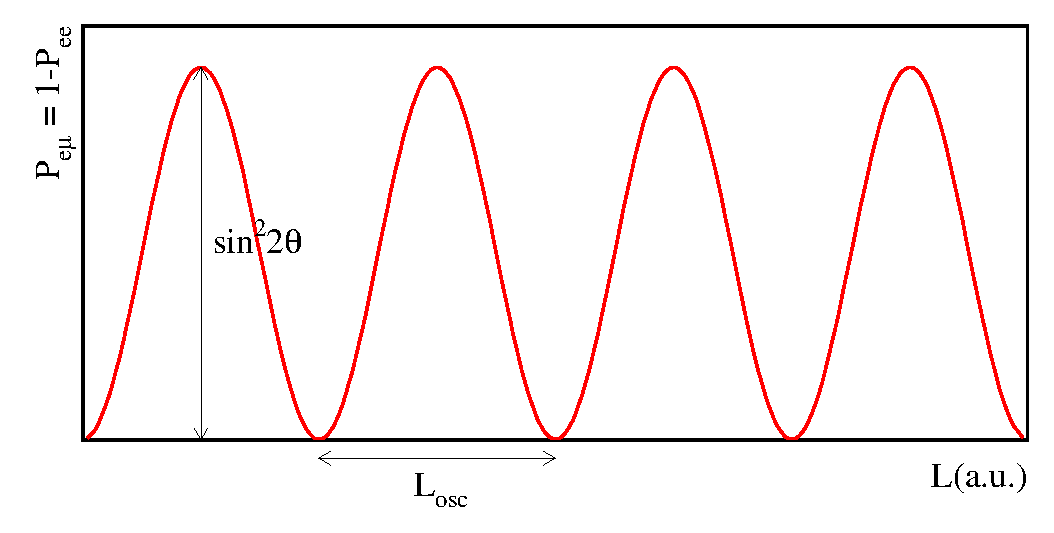
\includegraphics[height=6cm,width=8cm]{eps/osc1.eps}
\caption{$P_{e\mu}$ in funzione di $L$ per valori fissati di
$E$, $\Delta m^2$ e $\sin^2 2\theta$. }
\label{fig:osci_fixed}
\end{center}
\end{figure}


Le probabilit� di transizione descritte dalle equazioni \ref{eq:osci_2flavee} 
e \ref{eq:osci_2flav}
dipendono da due parametri. Il primo, $\theta$, non dipende dalla distanza
percorsa dal neutrino; $sin^2{2\theta}$ descrive l'ampiezza di
oscillazione dei neutrini. L'ampiezza � massima (uguale a uno) quando
l'angolo di mescolamento � $\theta=45�$, che quindi corrisponde al
mescolamento massimo. Quando $\theta=90�$, gli autostati di sapore
sono allineati con gli autostati di massa, il che corrisponde al
mescolamento minimo.  Il secondo fattore oscilla con il tempo, ovvero
la distanza $L$ percorsa dal neutrino. La fase del seno �
proporzionale alla differenza della massa degli autostati, $\Delta
m^2/4E$ e alla distanza $L$. Quindi per avere un'apprezzabile
probabilit� di transizione il termine di fase non deve essere troppo
piccolo.


 \section{Oscillazioni a tre sapori}
Per tre sapori di neutrino, la matrice di mescolamento � definita come
\begin{equation}
\begin{pmatrix}
\nu_e\\
\nu_\mu\\
\nu_\tau
\end{pmatrix}= \begin{pmatrix}U_{e1}&U_{e2}&U_{e3}\\ 
U_{\mu1}&U_{\mu2}&U_{\mu3}\\U_{\tau1}&U_{\tau2}&U_{\tau3}
\end{pmatrix}\begin{pmatrix}
\nu_1\\ \nu_2\\ \nu_3
\end{pmatrix}
\end{equation}
dove gli elementi devono soddisfare la condizione di unitariet\`a
 della matrice. Possiamo rappresentare gli elementi in termini di tre
 angoli di mescolamento $\theta_{12}$, $\theta_{13}$, $\theta_{23}$ e
 di una unica fase ineliminabile $\delta$ tramite le seguenti
 trasformazioni:

\begin{eqnarray}
\frac{|U_{e2}|^2}{U_{e1}|^2}&\equiv&\tan^2\theta_{12}\\
\frac{|U_{\mu3}|^2}{|U_{\tau3}|^2}&\equiv&\tan^2\theta_{23}\\
U_{e3}&\equiv&\sin\theta_{13}e^{-i\delta}
\end{eqnarray}

Possiamo utilizzare le convenzioni $m^2_2 > m_1^2$, e $\Delta
m^2_{12}<<|\Delta m^2_{13}|$. In questo caso abbiamo tre osservabili:
$\Delta m^2_{12}$, $|\Delta m^2_{13}|$ e il segno di $\Delta
m^2_{13}$. Il segno positivo di $\Delta m^2_{13}$ implica
$m^2_3>m^2_2>m_1^2$, definita anche gerarchia normale delle masse. Un
segno negativo implica $m^2_3<m^2_1<m^2_2$ definita gerarchia inversa
delle masse. Le due differenti gerarchie di massa sono mostrate in
figura~\ref{fig:mass_ger}.


\begin{figure}[!tbp]
\begin{center}
\includegraphics[height=6cm,width=8cm]{eps/3nuspic.eps}
\caption{Gerarchia delle masse dei neutrini.}
\label{fig:mass_ger}
\end{center}
\end{figure}

I recenti dati sperimentali sull'oscillazione dei neutrini danno
indicazione per un rapporto $\Delta m^2_{12}/|\Delta m^2_{13}\lesssim
1/30$. La probabilit� di oscillazione pu� essere scritta
come
\begin{equation}
P_{\alpha\beta}=\delta_{\alpha\beta}+A^{sol}_{\alpha\beta}
sin^2\left(\frac{\Delta
m^2_{12}L}{4E}\right)+A^{atm}_{\alpha\beta}\sin^2\left(\frac{\Delta
m^2_{13}L}{4E}\right)+ F^{int}_{\alpha\beta}(L,\Delta m^2_{12},\Delta
m^2_{13})
\end{equation}

In particolare, la probabilit\`a di sopravvivenza dei neutrini muonici
\`e data da:
\begin{equation}
P_{\mu\mu}\simeq 1-4|U_{\mu3}|^2(1-|U_{23}|^2)
\sin^2\left(\frac{\Delta m^2_{13}L}{4E}\right)
\label{eq:osci_atm}
\end{equation}
 Come vedremo questa probabilit\`a \`e rilevante per lo studio delle
 oscillazioni dei neutrini atmosferici.

Per la sparizione di (anti)neutrini di tipo elettronico (come quelli
provenienti dal reattore presso cui si � svolto l'esperimento CHOOZ)
si ha:
\begin{equation}
 P_{ee}\simeq
 1-4|U_{e3}|^2(1-|U_{e3}|^2)\sin^2\left(\frac{\Delta
 m^2_{13}L}{4E}\right)
\label{eq:osc_chooz}
\end{equation}

Essendo piccolo il valore misurato dell'angolo di mescolamento
$\theta_{13}$ ($\sin^2\theta_{13}\leq 0.047$, le oscillazioni
tra le famiglie 1-2 e 2-3 sono praticamente disaccoppiate e quindi le
equazioni~\ref{eq:osc_chooz} e \ref{eq:osci_atm} sono simili a quelle
trovate nel modello a due sapori.

Fino ad ora, abbiamo discusso
esclusivamente delle oscillazioni di neutrino nel vuoto. Per
comprendere le recenti osservazioni sperimentali ottenute dallo studio
dei neutrini solari ed atmosferici, alcune parole devono essere dette a
proposito delle oscillazioni di neutrino nella materia. Se il neutrino
si propaga nella materia, come accade quando esso attraversa il sole o
la terra, il fenomeno dell'oscillazione pu� significativamente
differire rispetto al caso del vuoto. La materia pu� aumentare il
mescolamento dei neutrini e la probabilit� di oscillazione nella materia
pu� essere grande anche se l'angolo di mescolamento nel vuoto � molto
piccolo: questo fenomeno � noto come effetto
Mikheyev-Smirnov-Wolfenstein (MSW). L'effetto � dovuto alle
differenti interazioni dei tre sapori di neutrini nella materia. Tutti
i sapori di neutrino interagiscono con gli elettroni, protoni e neutroni del mezzo
tramite interazioni di corrente neutra, mentre solo i $\nu_e$
interagiscono tramite correnti cariche con gli elettroni presenti. 

\section{Neutrini solari}
Il primo esperimento a produrre evidenza in favore dell'oscillazione
di neutrino fu una ricerca di neutrini solari condotta nella miniera
di Homestake nei primo anni 70 \cite{Homestake}. L'energia del sole \`e
sostanzialmente prodotta nelle reazioni dei cicli
nucleari $pp$ (fig.~\ref{fig:pp_cycle}) che producono neutrini di
tipo elettronico. Il flusso di $\nu_e$ solari \`e stato calcolato in
diversi modi nell'ambito del cosiddetto Modello Solare Standard \cite{MSS}. Tutti
questi calcoli si accordano piuttosto bene e le loro predizioni sono
anche confermate da misure di eliosismologia.  Dopo l'esperimento di
Homestake, altri esperimenti hanno misurato il flusso dei neutrini
elettronici di provenienza solare usando diverse tecniche sperimentali
e con diverse soglie di energia. I risultati di tali esperimenti
riportano un deficit rispetto alle predizioni che si aggira dal 30 al
60\%. Questo costitu� il cosiddetto problema dei neutrini solari.

\begin{figure}[!tbp]
\begin{center}
\includegraphics[height=16cm,width=14cm]{eps/ciclopp.ps}
\caption{Ciclo $pp$ diviso in tre sottocicli. }
\label{fig:pp_cycle}
\end{center}
\end{figure}
Dagli esperimenti Homestake~\cite{clorine}, Gallex~\cite{gallium},
Super-Kamiokande~\cite{SK} e SNO~\cite{sno} risulta ora stabilito in
maniera convincente che il deficit di $\nu_e$ solari osservati implica
nuova fisica nel settore dei neutrini. Escludendo neutrini sterili e
interazioni non convenzionali, tale deficit pu\`o infatti essere
spiegato dall'ipotesi di oscillazioni nel canale $\nu_e
\rightarrow \nu_{\alpha}$, dove $\nu_{\alpha}$ \`e una combinazione
lineare di $\nu_{\mu}$ e $\nu$. Negli esperimenti citati queste
oscillazioni si manifestano come una ``sparizione'' di $\nu_e$, che
sostanzialmente portano a una misura dei parametri $\theta_{12}$ e
$\Delta m^2_{12}$.

Grazie all'uso di acqua pesante e quindi di un bersaglio contenente deuterio,
l'esperimento SNO ha inoltre permesso di
paragonare le frequenze delle interazioni di corrente carica e neutra,
in particolare sono state utilizzate per queste osservazioni reazioni
di corrente carica accessibili solo ai $\nu_e$ e reazioni di corrente
neutra accessibili a tutti e tre i sapori (\cite{ccsno} e
\cite{ncsno}). Confrontando il rapporto osservato delle interazioni di
corrente carica su quelle di corrente neutra con quello atteso, SNO ha
confermato che il deficit di neutrini solari \`e dovuto alle
oscillazioni di neutrini $\nu_e$ in altro sapore e non ad una cattiva
predizione del modello solare.  Nel settembre 2003 sono stati
pubblicati nuovi risultati di SNO ottenuti aggiungendo sale all'acqua
pesante del loro rivelatore in modo da aumentare la sensibilit\`a al
canale di corrente neutra. I risultati precedentemente ottenuti sono
stati confermati \cite{sno} con accuratezza maggiore: attualmente le
transizioni di $\nu_e$ sono confermate con un livello di significanza
statistica di oltre 5$\sigma$.

L'esperimento CHOOZ~\cite{chooz} ha ricercato la sparizione di
$\bar{\nu}_e$ utilizzando un reattore nucleare. I suoi risultati sono
combinati con quelli degli esperimenti di neutrini solari. Tali
risultati portano a dare un limite superiore sull'angolo $\theta_{13}$
($sen{\theta_{13}} < 0.10$ al 90\% CL) sicch\'e viene tuttora
considerato nullo. La sua misura � uno dei temi dominanti delle
ricerche future. 

L'esperimento KamLAND~\cite{kamland} ha ricercato
oscillazioni di neutrini su lunga base nella regione di masse di
interesse per i neutrini solari, rivelando antineutrini prodotti da
reattori situati sul territorio giapponese. I risultati hanno
confermato le osservazioni dei neutrini solari migliorando
notevolmente la misura dei parametri di oscillazione. In
figura~\ref{fig:lma} \`e riportata la regione dei parametri di
oscillazione che emerge dall'analisi combinata di CHOOZ, KamLAND e dei
neutrini solari. La soluzione a grandi angoli di mescolamento LMA-I
\`e chiaramente preferita dai dati. Recentemente KamLAND
\cite{Kamland} ha pubblicato nuovi risultati ottenuti con un aumento
di statistica. Sono stati osservati 258 eventi di $\bar{\nu}_e$ contro
365.2 eventi attesi in assenza di oscillazioni di neutrino. KamLAND
non solo \`e stato in grado di scegliere la regione LMA preferita ma
ha potuto significativamente restringere la corrispondente regione dei
parametri di oscillazione ottenendo:
$$\Delta m_{12}^2 =7.9^{+0.6}_{-0.5}\times
10^{-5}eV^2~~~~~~~~~~~tan^2\theta_{12}=0.40^{+0.10}_{-0.07}$$

\begin{figure}[!tpb]
\begin{center}
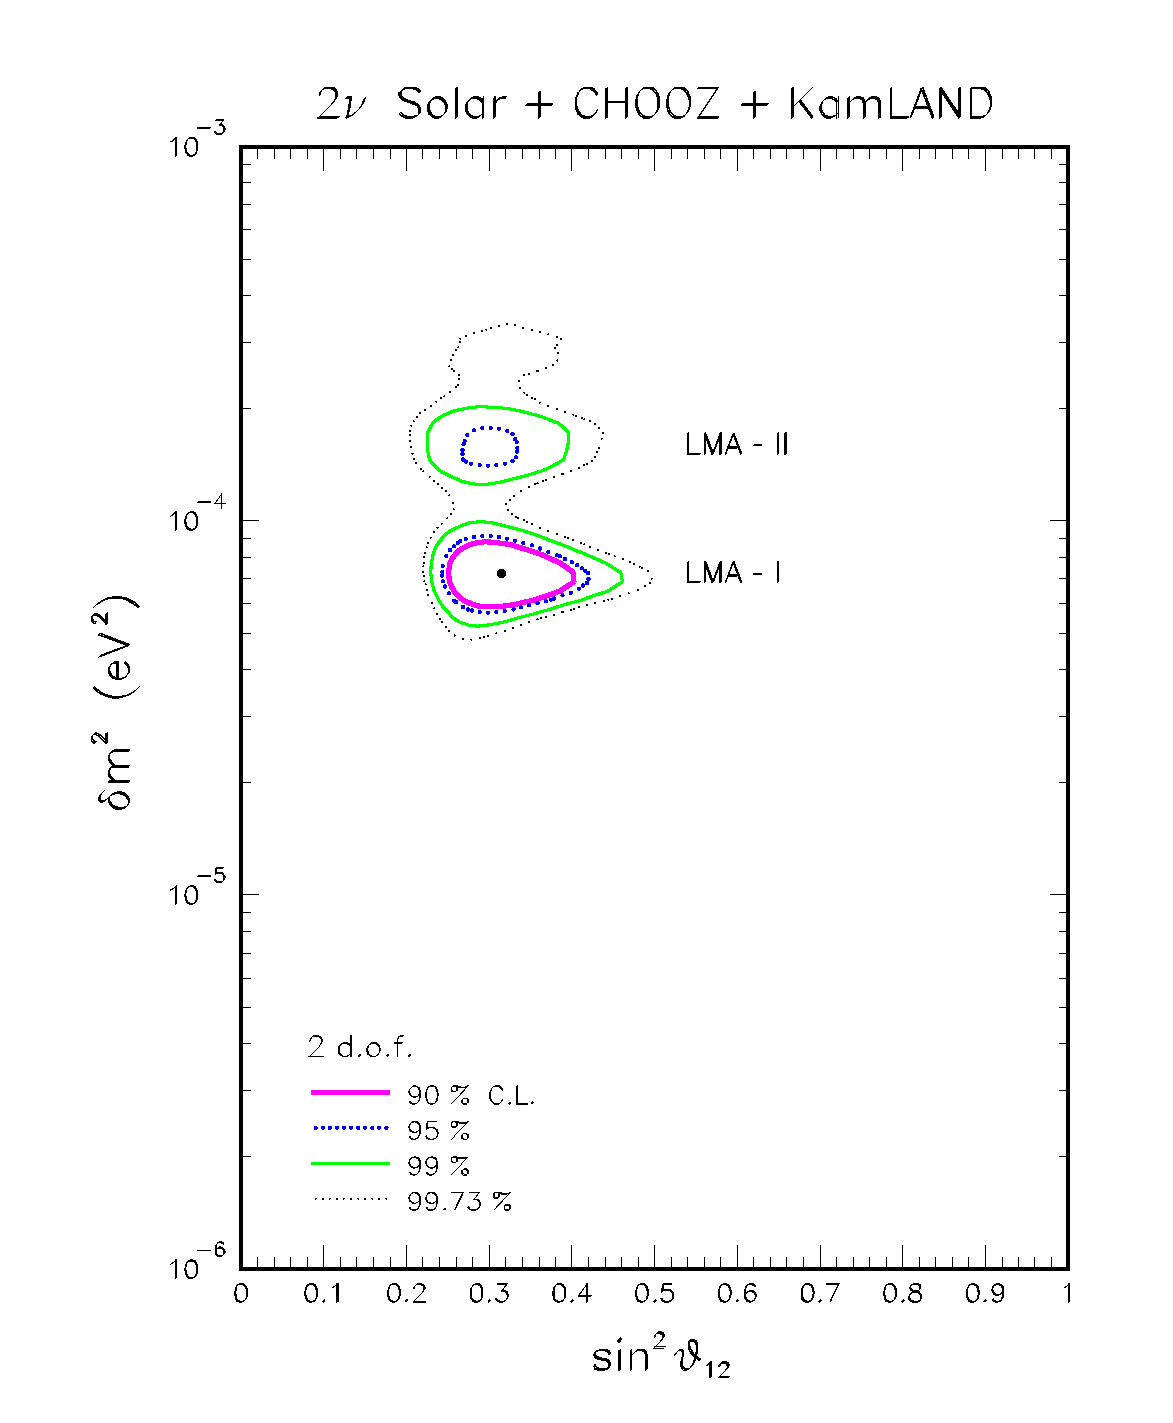
\includegraphics[height=16cm,width=14cm]{eps/LMA-I-II.eps}
\caption{Analisi globale dei esperimenti CHOOZ, KamLAND e dei neutrini
  solari nella regione dei parametri $\theta_{12}$ e $\Delta
  m^2_{sun}$. }
\label{fig:lma}
\end{center}
\end{figure}

\section{Neutrini atmosferici}


I neutrini atmosferici sono neutrini e antineutrini di tipo
elettronico e muonico prodotti nelle cascate adroniche indotte dai
raggi cosmici primari nell'atmosfera terrestre. La principale
produzione di neutrini avviene attraverso la seguente catena:
\begin{equation}
\begin{array}{lllll}
p(\alpha, ...)+Air&\rightarrow &\pi^{\pm}(K^{\pm})&+ & X  \\
&   &\pi^{\pm}(K^{\pm})&\rightarrow
&\mu^{\pm}+\nu_{\mu}(\bar{\nu}_{\mu})\\
& & & &\mu^{\pm}\rightarrow e^{\pm}+\nu_{e}(\bar{\nu}_{e})+
\bar{\nu}_{\mu}(\nu_{\mu})
\end{array}
\label{eq:atm_neut_chain}
\end{equation}

Dalla reazione \ref{eq:atm_neut_chain} possiamo aspettarci di avere
due neutrini o antineutrini muonici per ogni neutrino o antineutrino
elettronico. La prima generazione di rivelatori, NUSEX, Soudan, IMB,
Frejus e Kamiokande ha misurato il rapporto tra $\nu_\mu /\nu_e$ atteso
dal MonteCarlo e quello misurato, ovvero il doppio rapporto:
\begin{equation}
R(\nu_\mu/\nu_e)\equiv
\dfrac{[(\nu_{\mu}+\bar{\nu}_{\mu})/(\nu_e+\bar{\nu}_e)]_{data}}{[(
\nu_\mu+\bar{\nu}_{\mu})/(\nu_e+\bar{\nu}_e)]_{MC}}
\end{equation}

Soudan, IMB e Kamiokande hanno misurato un valore
inferiore a quello atteso compatibile con una ipotesi di
oscillazione. La discrepanza tra il valore atteso e quello misurata va
sotto il nome di anomalia dei neutrini atmosferici. Oltre a questa
anomalia, Kamiokande ha anche dato una prima importante indicazione di una sua dipendenza
azimutale, collegabile a una diversa distanza tra la produzione dei neutrini nell'atmosfera
e la loro osservazione nel rivelatore.  Questa osservazione forn� una ulteriore indicazione 
di oscillazioni di neutrino.

Una seconda generazione di esperimenti,
SuperKamiokande~\cite{SKa}, Soudan-2~\cite{soudan2} e
MACRO~\cite{macro} ha condotto approfondite osservazioni di
 questo fenomeno e studiato il
deficit in relazione all'azimuth di provenienza del neutrino.
 Questi esperimenti hanno utilizzato
diverse tecniche per identificare il leptone dello stato finale in
interazioni di corrente carica di neutrino. Soudan-2 e MACRO hanno
usato un rivelatore calorimetrico tracciante. SuperKamiokande, tuttora in funzione, usa un
rivelatore di luce Cherenkov in acqua. Questi esperimenti hanno
confermato la spiegazione dell'anomalia dei
neutrini atmosferici in termini di oscillazioni di
neutrino.  

In particolare, Superkamiokande ha evidenziato una chiara
discrepanza rispetto alle predizioni fatte in assenza di oscillazioni
 nella distribuzione dell'angolo azimutale per
eventi con presenza di un muone, mentre nel caso di eventi con
elettrone non si osserva alcuna discrepanza. Questa � una
evidenza che l'anomalia dei neutrini atmosferici � una
conseguenza di una oscillazione, presumibilmente $\nu_\mu \rightarrow \nu_\tau$ 
vista l'assenza di apprezzabili anomalie nel flusso di $\nu_e$ (fig. \ref{fig:sk}).

\begin{figure}[!tpb]
\begin{center}
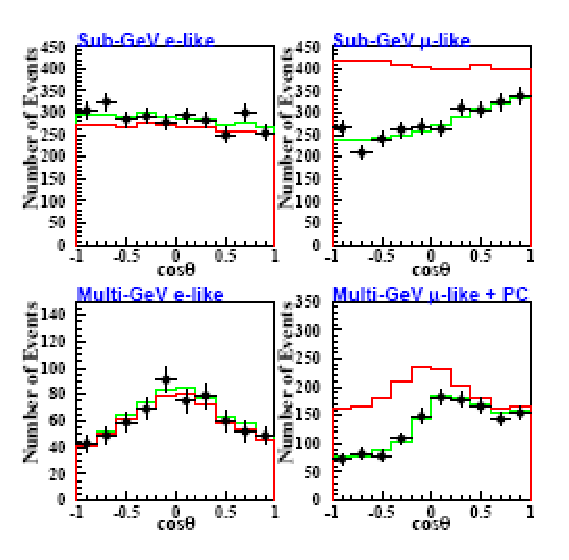
\includegraphics[height=16cm,width=14cm]{eps/SK.eps}
\caption{Distribuzione del coseno dell'angolo azimutale ottenuta da Super Lamiokande per eventi con elettrone (sinistra) ed eventi con muone (destra). La linea rossa \`e la distribuzione attesa in assenza di oscillazioni, mentre la linea verde rappresenta il caso di oscillazioni $\nu_\mu\rightarrow\nu_\tau$ con mescolamento massimale e $\Delta m^2_{23}=2.5\times~10^{-3}~eV^2$.}
\label{fig:sk}
\end{center}
\end{figure}

I risultati di SuperKamiokande sono stati riprodotti indipendentemente
da un esperimento con fascio di neutrini terrestri:
K2K~\cite{k2k}. In tale esperimento, neutrini di energia media di
1.3 GeV sono inviati sul rivelatore di Superkamiokande, a una distanza di 250 Km
dal luogo di produzione dei neutrini. La figura~\ref{fig:skk2k}
\begin{figure}[h]
\begin{center}
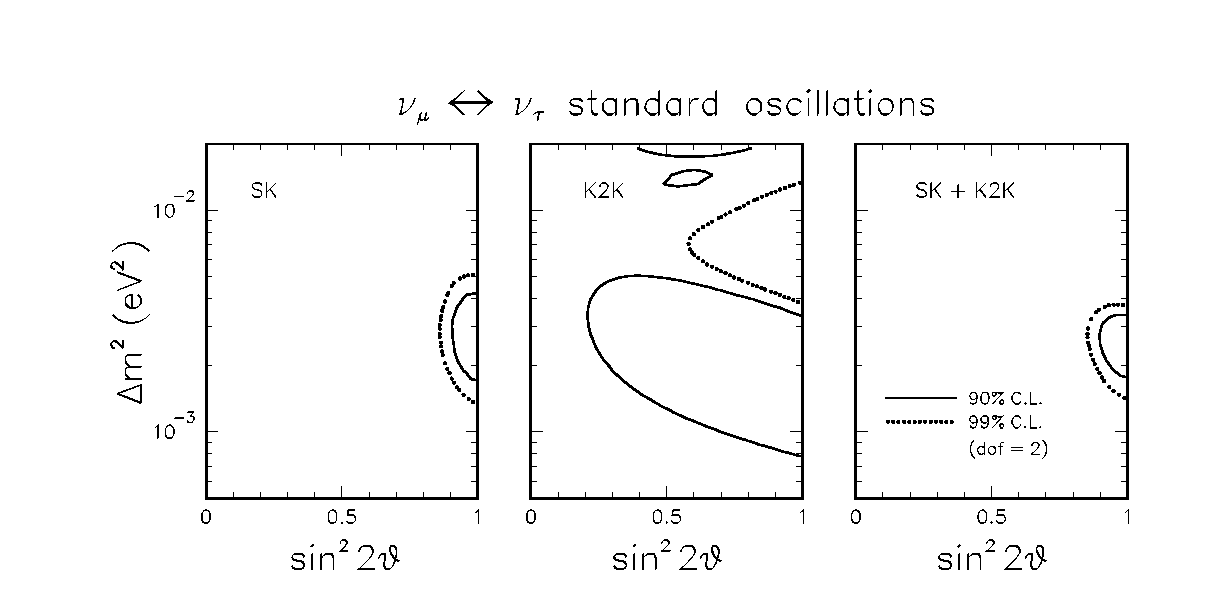
\includegraphics[height=16cm,width=14cm]{eps/SK_K2K.eps}
\caption{Oscillazioni nel canale $\nu_{\mu} \rightarrow \nu_{\tau}$:
  limiti alle regioni dei parametri $\theta_{23}$ e $\Delta
  m^2_{atm}$ provenienti dagli esperimenti SuperKamiokande e K2K. }
\label{fig:skk2k}
\end{center}
\end{figure}
mostra le regioni dei parametri consentiti in base ai dati degli
esperimenti K2K e SuperKamiokande. K2K ha prodotto un rafforzamento  del
limite superiore sulla differenza di masse. La figura~\ref{fig:k2knew}
\begin{figure}[h]
\begin{center}
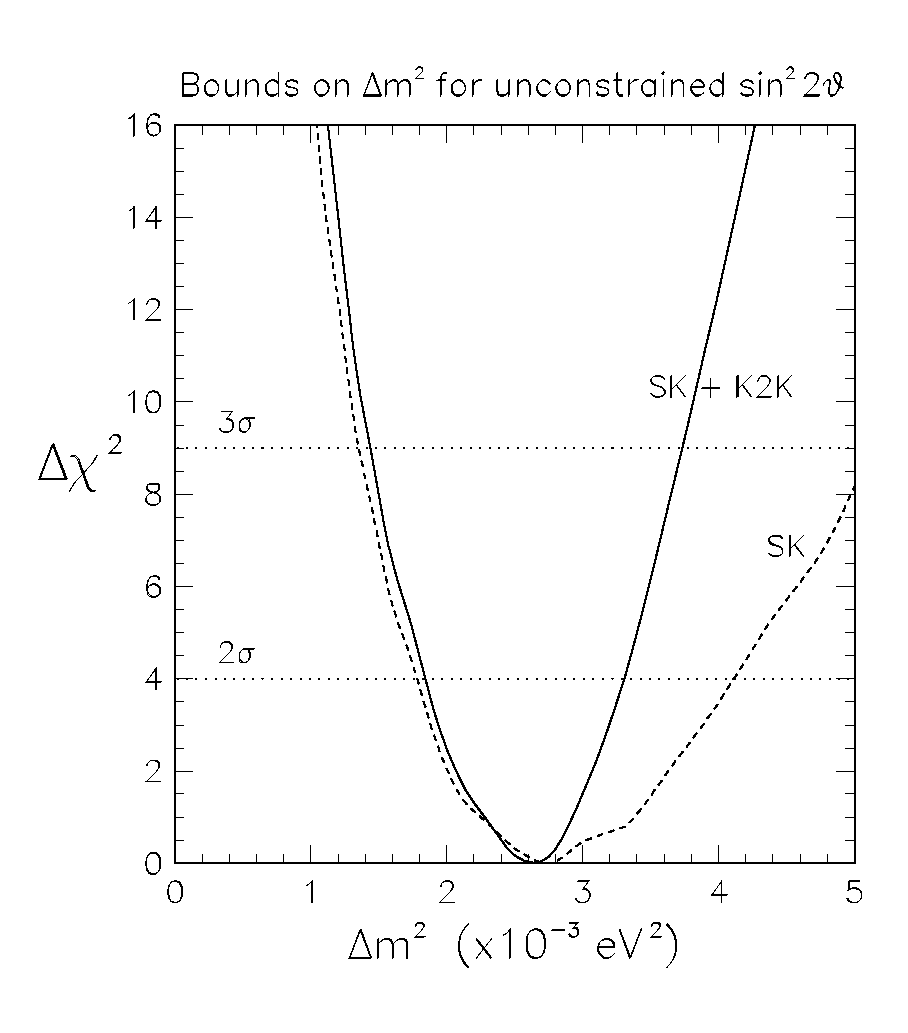
\includegraphics[height=16cm,width=14cm]{eps/SK_K2K_proj_dm2.eps}
\caption{Oscillazioni nel canale $\nu_{\mu} \rightarrow \nu_{\tau}$:
sono riportati i limiti su $\Delta m^2_{atm}$ vincolando
$\theta_{23}$. I dati sono di K2K e SuperKamiokande.}
\label{fig:k2knew}
\end{center}
\end{figure}
mostra i limiti sui valori consentiti di $\Delta m^2_{atm}$ eliminando
la dipendenza da $\theta_{23}$, ovvero assumendo $sen^2{2\theta_{23}}
= 1$. Il fit globale ai dati di K2K e SuperKamiokande mostra un andamento
pressoch\'e quadratico di $\Delta \chi^2 \equiv \chi^2 -\chi^2_{min}$
in funzione di $\Delta m^2$ fino a circa 3$\sigma$, con un minimo per $\Delta m^2$ = $2.6
\times 10^{-3}$eV$^2$. Il valore preferito per $sen^2{2\theta_{23}}$ \`e
$1.00^{+0.00}_{-0.05}$. 

\section{L'esperimento LNSD}
L'esperimento LSND (Liquid Scintillator Neutrino Detector), progettato
per la ricerca di $\bar{\nu_\mu} \rightarrow \bar{\nu_e}$, ha
riportato nel 1995 un eccesso di eventi con elettrone sul fondo
stimato, dando un'interpretazione di questo risultato in termini di
oscillazioni di neutrino. Questa interpretazione comporta
l'introduzione di una terza frequenza di oscillazione associata ad uno
o pi� neutrini sterili. Tuttavia questa ipotesi non � ancora supportata
da altri esperimenti. L'esperimento MiniBoone presto fornir� un
chiarimento sul segnale visto da LNSD.

\section{Sintesi dei risultati e prospettive future}


Analisi combinate dei dati sperimentali evidenziano l'oscillazione di
neutrini con i seguenti valori dei parametri dati con intervallo di
confidenza a 3 sigma, 
\begin{itemize}
\item{$0.22 < \sin^2\theta_{12} < 0.38$, da neutrini solari}
\item{$0.32 < \sin^2 \theta_{23} < 0.68$, da neutrini atmosferici}
\item{$\sin^2\theta_{13}\leq 0.047$, da neutrini atmosferici e CHOOZ}
\item{$7.1 < \Delta m^2_{12} < 9.1 eV^2$, da KamLand e SuperKamiokande}
\item{$1.5 < |\Delta m^2_{13}| < 3.6 eV^2$, da neutrini atmsferici e K2K}
\end{itemize}
Questi risultati sono riassunti nella figura~\ref{fig:som_data}.

\begin{figure}[p]
\begin{center}
\includegraphics[height=6cm,width=8cm]{eps/summary.eps}
\caption{Proiezione delle regioni dei parametri di
oscillazioni. $\Delta \chi^2 = \chi^2 -\chi^2_{min}$.}
\label{fig:som_data}
\end{center}
\end{figure}


L'analisi mostra che lo scenario sperimentale delle oscillazioni di
neutrino lascia aperti importanti quesiti. Una particolare attenzione
va rivolta alla piena comprensione del segnale di oscillazione
proveniente dai neutrini atmosferici. In questo quadro si
inseriscono i programmi di ricerca con fasci di $\nu_\mu$ prodotti da
acceleratori e con esperimenti a $long~baseline$, cio� con $L/E$
relativamente grande. 

Le osservazioni di SuperKamiokande hanno come plausibile
origine una oscillazione $\nu_\mu\rightarrow\nu_\tau$. Un esperimento
che riveli direttamente una apparizione di $\nu_\tau$ �, quindi, di grande
importanza per confermare questa ipotesi. L'esperimento MINOS sul fascio NuMI del Fermilab negli USA 
si ripromette di misurare con maggiore precisione i parametri di oscillazione, ma potr� vedere
solo un effetto indiretto e cio� un apparente eccesso di interazioni
di corrente neutra rispetto a quanto atteso in un fascio di neutrini
puramente muonici. L'esperimento OPERA sul fascio CNGS dal CERN al
Gran Sasso ha l'ambizioso obiettivo di osservare l'apparizione di $\nu_\tau$,
 attraverso l'osservazione
diretta della loro interazione per corrente carica e del decadimento del $\tau$ prodotto.











\chapter{L'esperimento OPERA}

\section{Esperimenti con acceleratori nel dominio di massa indicato dai neutrini atmosferici}

Nel capitolo precedente si \`{e} visto che le attuali evidenze sperimentali per le oscillazioni 
di neutrino vengono da osservazioni fatte con neutrini solari, recentemente confermate 
dall'esperimento Kamland \cite{Kamland} operante con neutrini provenienti da reattori nucleari, e da 
osservazioni fatte con neutrini atmosferici. L'eccesso di eventi indotti da $\overline{\nu }_{e}$ rilevato
dall'esperimento LSND \cite{A32} e imputabile a oscillazioni di neutrino resta non confermato da altri
esperimenti.

Nel caso dei neutrini atmosferici, i risultati sperimentali conducono
a suggerire l'esistenza di oscillazioni $\nu _{\mu }\rightarrow \nu
_{\tau }$ nella regione dei parametri corrispondente a $\Delta m^{2} =
( 1.5\div 3.4) \times 10^{-3}$ $eV^{2}$ e $\sin ^{2}2\theta \sim
1$. Vengono invece sfavoriti il canale $\nu _{\mu }\rightarrow \nu
_{e}$ e l'oscillazione di $\nu _{\mu } $ in neutrini sterili, cio\`{e}
non visibili tramite le interazioni deboli.

Per esplorare con fasci prodotti da acceleratori di particelle il suddetto dominio dei parametri 
di oscillazione, con valori
di $\Delta m^{2}$ cos\`{i} bassi, sono necessari esperimenti con un rapporto $\frac{L}{E%
}$ che si approssimi a quello dei neutrini atmosferici, ove $L$ \`{e} la distanza tra
sorgente e rivelatore ed $E$ \`{e} l'energia del fascio, e quindi con un distanza sorgente-rivelatore 
relativamente alta. Sono questi i cosiddetti esperimenti a \emph{long baseline} (LBL). 

E' possibile dimostrare, infatti, che in presenza di fondo la sensibilit\`{a} in $\Delta
m^{2}$ di un esperimento di apparizione migliora con la radice quadrata di $L$. 
\`{E} solo nel caso ideale di assenza di fondo che essa risulta
indipendente da $L$, migliorando con la radice quadrata
della massa del rivelatore e con l'inverso dell'energia. In generale, gli esperimenti su long baseline, 
traggono notevole vantaggio dalla grande distanza del rivelatore dalla sorgente del fascio, che riduce
drasticamente il numero di eventi di fondo.

La figura 2.1 mostra le regioni del piano $\sin ^{2}2\theta -\Delta m^{2}$
esplorabili con esperimenti a LBL e con esperimenti a {\emph{short baseline}} (SBL).

\begin{figure}[tbp]
\begin{center}
\includegraphics[width=80mm,height=95mm]{./figure_cap2/figura2_1.eps}
\end{center}
\caption{Regioni esplorabili con esperimenti LBL e SBL.}
\end{figure}

 Uno dei principali ostacoli alla realizzazione di 
esperimenti a LBL \`{e} indotto dalla naturale divergenza del fascio, che
riduce fortemente il flusso di neutrini che giungono al rivelatore. Il
flusso emesso da una sorgente, infatti, pu\`{o} essere scritto come:

\begin{equation}
\Phi =\frac{dN_{\nu }}{dA}  \tag{2.1}
\end{equation}
dove $dN_{\nu }$ indica il numero di neutrini che, nell'unit\`{a} di tempo,
attraversano una superficie di area $dA$ disposta perpendicolarmente al fascio. Per
un angolo solido $d\Omega $ si ha:

\begin{equation}
dA=L^{2}\cdot d\Omega  \tag{2.2}
\end{equation}
che, unita alla (2.1), fornisce:

\begin{equation*}
\Phi \propto \frac{1}{L^{2}}
\end{equation*}
Il flusso risulta quindi inversamente proporzionale al quadrato della
distanza.

Ad esempio, in un esperimento LBL con $L\simeq 10^{3}$ $Km$ il flusso
di neutrini che giunge al rivelatore risulta circa un milione di volte
pi\`{u} basso di quello in un esperimento con $\% L\simeq 1$ $Km$ che
utilizzi lo stesso rivelatore sulla stessa linea del fascio.  Di
conseguenza, se con un esperimento SBL si prevede di rivelare, in un
certo periodo di tempo, un numero di eventi di corrente carica $\nu_\mu$ 
dell'ordine di $10^{6}$, in un esperimento LBL, operante con lo
stesso bersaglio e sulla medesima linea di fascio, si otterr\`{a} un
solo evento. Ci\`{o} significa, inoltre, che se la massa del
rivelatore SBL \`{e} dell'ordine di $1$ $ton$ (come in CHORUS e
NOMAD), per un esperimento LBL con un bersaglio di massa $\sim 1$
$kton$ si ha un numero di eventi inferiore di circa tre ordini di
grandezza.

Gli obbiettivi della prossima generazione di esperimenti volti ad
approfondire mediante l'uso di fasci prodotti da acceleratori lo
studio degli effetti osservati con neutrini atmosferici sono
l'osservazione diretta di oscillazioni $\nu_\mu \rightarrow \nu_\tau$
tramite apparizione di $\nu_\tau$ e una misura piu' precisa dei
parametri di oscillazione.  Nei limiti della sensibilita' degli
esperimenti, verra' inoltre ricercata la presenza di oscillazioni
"sub-dominanti" $\nu_\mu \rightarrow \nu_e$.

Negli Stati Uniti il progetto \textbf{NuMI} \cite{B1} prevede l'invio
dei neutrini muonici dal Fermilab (FNAL) alla miniera Soudan nel
Minnesota (posta ad una distanza di $730$ $Km$) in cui \`{e} situato
il rivelatore MINOS \cite{B2}. Questo rivelatore e' essenzialmente uno
spettrometro per muoni, costituito da lastre di ferro magnetizzato per
una massa di $5.4$ $kton$. Si tratta di un esperimento di sparizione
di $\nu _{\mu }$, dunque l'oscillazione $% \nu _{\mu }\rightarrow \nu
_{\tau }$ puo' venire misurata soltanto in termini di eccesso
statistico di eventi senza muone nello stato finale. L'apparato
sperimentale e' inoltre in grado di osservare eventi con elettrone
nello stato finale, pur non essendo ottimizzato per questo
scopo. Verra' quindi eseguita anche una ricerca di oscillazioni
$\nu_\mu\rightarrow \nu_e$. La presa dati sta ora iniziando.

In Europa, un progetto congiunto CERN - INFN prevede l'invio del fascio di
neutrini muonici del fascio CNGS \cite{B3} dal CERN ai Laboratori Nazionali del Gran
Sasso, posto ad un distanza $L\simeq 732$ $Km$. L'energia media del fascio (%
$E_{\nu }\simeq 17.7$ $GeV$) \`{e} ottimizzata per lo studio di apparizione $%
\nu _{\mu }\rightarrow \nu _{\tau }$. La ricerca di oscillazioni
 $\nu _{\mu }\rightarrow \nu _{\tau }$, basata
sulla ricerca diretta dell'apparizione, necessita infatti di fasci di $\nu _{\mu }$ dotati
di energia superiore alla soglia di produzione del leptone $\tau $ (ossia $%
E_{\nu }>3.6$ $GeV$).

Come per gli esperimenti SBL, sono possibili due approcci per la
rivelazione del $\tau $:

\begin{itemize}
\item  sfruttare esclusivamente le caratteristiche cinematiche peculiari del decadimento
del $\tau $;
\item  identificare il $\tau $ attraverso l'osservazione diretta del suo
decadimento e ricorrere allo studio della cinematica del decadimento solo per una
ulteriore riduzione del fondo.
\end{itemize}

Sul primo tipo di approccio si basa l'esperimento \textbf{ICARUS} \cite{B4},
il cui rivelatore si compone di quattro moduli, ciascuno dei quali \`{e}
costituito da una Time Projection Chamber (TPC) ad Argon liquido.

Il secondo approccio \`{e} quello seguito dall'esperimento \textbf{%
OPERA} \cite{B5}, al quale \`{e} dedicato il presente capitolo.

Ambedue gli esperimenti sono anche in grado di osservare eventi con un elettrone
nello stato finale e quindi di ricercare oscillazioni $\nu_\mu\rightarrow \nu_e$.

Il fascio CNGS verra' operato a partire da meta' del 2006.

\section{Il fascio CNGS}\label{sec:cngs}

Il fascio di neutrini \textbf{CNGS} (\textbf{C}\emph{ERN} \textbf{N}\emph{%
eutrino} \emph{to} \textbf{G}\emph{ran} \textbf{S}\emph{asso}) sar\`{a}
prodotto dal \textbf{SPS} (\textbf{S}\emph{uper} \textbf{P}\emph{roto} 
\textbf{S}\emph{incrotrone}) del CERN facendo interagire protoni accelerati un'energia
 di $400$ $GeV$ su un bersaglio costituito da 13 cilindri di carbonio di $10$ $cm$ di
lunghezza e $4$ $cm$ di diametro. I mesoni $\pi ^{+}$ e $K^{+}$ che ne
derivano saranno collimati lungo la direzione di volo verso il Gran Sasso,
mediante un sistema costituito da due lenti di focalizzazione e decadono
all'interno di un tunnel lungo $1$ $Km$. Alla fine del tunnel \`{e} posto  un %
\emph{hadron stop}, che ha il compito di assorbire i protoni che non hanno
interagito col bersaglio ed i mesoni che non sono decaduti entro il tunnel.
Esso \`{e} realizzato con un blocco, lungo $18$ $m$, di grafite e di ferro.
Per controllare il fascio di neutrini, saranno utilizzate due stazioni di
rivelatori al silicio, una posta subito dietro l'hadron stop, l'altra
separata da 67 metri di roccia.

La tabella 2.1 riporta le caratteristiche nominali del fascio. In figura
2.2 \`{e} mostrato lo schema della linea del fascio ed in figura 2.3 lo
spettro energetico dei neutrini $\nu _{\mu }$ attesi al Gran Sasso.

\begin{table}[tbp]
\begin{center}
\begin{tabular}{||c|c||}
\hline\hline
$\nu _{\mu }[m^{2}$ $pot]$ & $7.78\times 10^{-9}$ \\ \hline
$E_{\nu _{\mu }}[Gev]$ & $17.7$ \\ \hline
$\nu _{\mu }CC[eventi/pot/kt]$ & $5.85\times 10^{-17}$ \\ \hline
$\overline{\nu }_{\mu }/\nu _{\mu }$ & $2.1\%$ \\ \hline
$\nu _{e}/\nu _{\mu }$ & $0.8\%$ \\ \hline
$\overline{\nu }_{e}/\nu _{\mu }$ & $0.07\%$ \\ \hline
$\nu _{\tau }$ & \textbf{trascurabile} \\ \hline\hline
\end{tabular}
\end{center}
\caption{Caratteristiche nominali del fascio CNGS.}
\end{table}

\begin{figure}[tbp]
\begin{center}
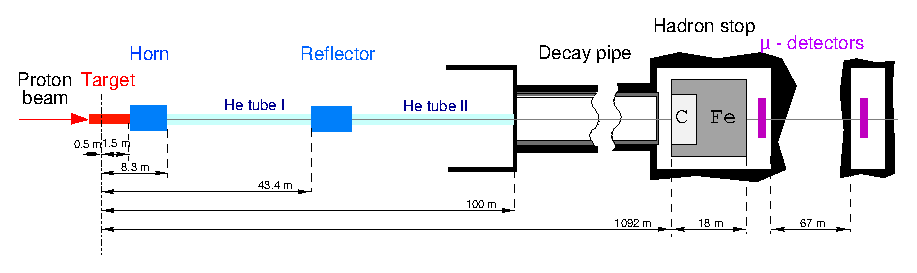
\includegraphics[width=130mm,height=40mm]{./figure_cap2/figura2_2.eps}
\end{center}
\caption[Struttura del fascio CNGS.]{Configurazione della linea di fascio CNGS}
\end{figure}

\begin{figure}[tbp]
\begin{center}
\includegraphics[width=80mm,height=75mm]{./figure_cap2/figura2_3.sh}
\end{center}
\caption{Spettro in energia del fascio di $\protect\nu _{\protect\mu }$ del
CNGS atteso al Gran Sasso.}
\end{figure}

Assumendo 200 giorni di funzionamento all'anno, il numero di \emph{pot}
(protoni su bersaglio) attesi operando il fascio assieme al collisionatore protone-protone
 LHC \`{e} pari a $4.5\times 10^{19}/anno$.

Il numero di interazioni da neutrino, includendo tutti i sapori e
considerando anche gli eventi di corrente neutra, \`{e} pari a $\sim 35000$%
, per un rivelatore di massa $1.8$ $kt$ e 5 anni di esposizione al fascio.
Il corrispondente numero di interazioni di corrente carica di $\nu _{\tau }$ \`{e}
pari a circa 130, per $\Delta m^{2}=2.4\times 10^{-3}$ $eV^{2}$ e mescolamento massimo
(ossia $\sin ^{2}2\theta =1$). Appare possibile che l'intensita' del fascio sia aumentata di un
fattore $1.5$ rispetto a quella nominale prevista nel progetto iniziale, a cui si riferiscono 
i suddetti numeri di interazioni.

\section{L'esperimento OPERA}

\textbf{OPERA} (\textbf{O}\emph{scillation} \textbf{P}\emph{roject with} 
\textbf{E}\emph{mulsion t}\textbf{R}\emph{acking} \textbf{A}\emph{pparatus})
\`{e} un esperimento per l'osservazione di oscillazioni $\nu _{\mu }\rightarrow \nu _{\tau }$
su \emph{ long baseline} nel
fascio CNGS, tramite la rivelazione dell'apparizione del $\nu
_{\tau }$ attraverso l'osservazione della produzione
del leptone $\tau $ (figura 2.4). La ricerca dell'apparizione del $\nu
_{\tau }$ viene effettuata nella regione
dei parametri indicata dalle osservazioni con muonici atmosferici. Il rivelatore e' posto
nei laboratori sotterranei del Gran Sasso, a circa $730$ $Km$ di distanza
dal CERN.
L'esperimento � sensibile anche alle oscillazioni di  $\nu_\mu \rightarrow\nu_e$,
in una regione di parametri di oscillazione pi� estesa rispetto agli esperimenti condotti
sino ad ora.

\begin{figure}[tbp]
\begin{center}
\includegraphics[width=130mm,height=40mm]{./figure_cap2/figura2_5.eps}
\end{center}
\caption{Schema delle oscillazioni dei neutrini provenienti dal CERN.}
\end{figure}

La rivelazione del $\nu _{\tau }$ consente di identificare l'avvenuta
oscillazione $\nu _{\mu }\rightarrow \nu _{\tau }$, in quanto il fascio
proveniente dal CERN non contiene neutrini in misura apprezzabile  $\nu _{\tau }$.
Anche pochi eventi di segnale possono essere sufficienti a dimostrare
l'ipotesi di oscillazione, purch\'{e} il fondo venga mantenuto sempre ad un
basso livello.

In OPERA, lo strumento di base per la reiezione del fondo e' l'osservazione del decadimento del tau.
Il leptone tau ha una vita media breve ($c\tau \sim 87$ $\mu m$). In base alla
distribuzione in energia del fascio CNGS, si ottiene la distribuzione delle
lunghezze di decadimento del $\tau $ riportata in figura 2.5. Alle energie del CNGS,
 il leptone $\tau $ decade in media dopo circa $0.5 mm$. Per osservare sia la produzione che 
il decadimento del
leptone tau occorre quindi utilizzare una tecnica che offra altissime 
granularita' e risoluzione spaziale. Le tecnica delle \emph{ emulsioni nucleari}
presenta caratteristiche uniche
 sotto questo aspetto. Dopo lo sviluppo, i "grani" delle emulsioni hanno dimensioni dell'ordine
 del micron e permettono di ottenere risoluzioni sub-micrometriche.
 
L'utilizzo di emulsioni nucleari ha importantissimi precedenti nella
fisica delle particelle elementari, in particolare per l'osservazione
di particelle a vita breve.  Fu lo sviluppo di questa tecnica che
permise nel 1947 la scoperta del pione attraverso il suo decadimento
in muone nell'esperimento Lattes-Occhialini-Powell \cite{pione}. La
prima osservazione delle particelle poi definite come "charmate" dopo
la loro chiarissima osservazione al BNL e a SLAC \cite{jpsi1,jpsi2,jpsi3}
avvenne nel 1971 in un esperimento con raggi cosmici in cui erano
utilizzate emulsioni nucleari \cite{Niu}. L'esperimento WA75 at CERN
effetuo' la prima osservazione diretta del decadimento di una
particella dotata di "beauty" \cite{beauty}

\begin{figure}[tbp]
\begin{center}
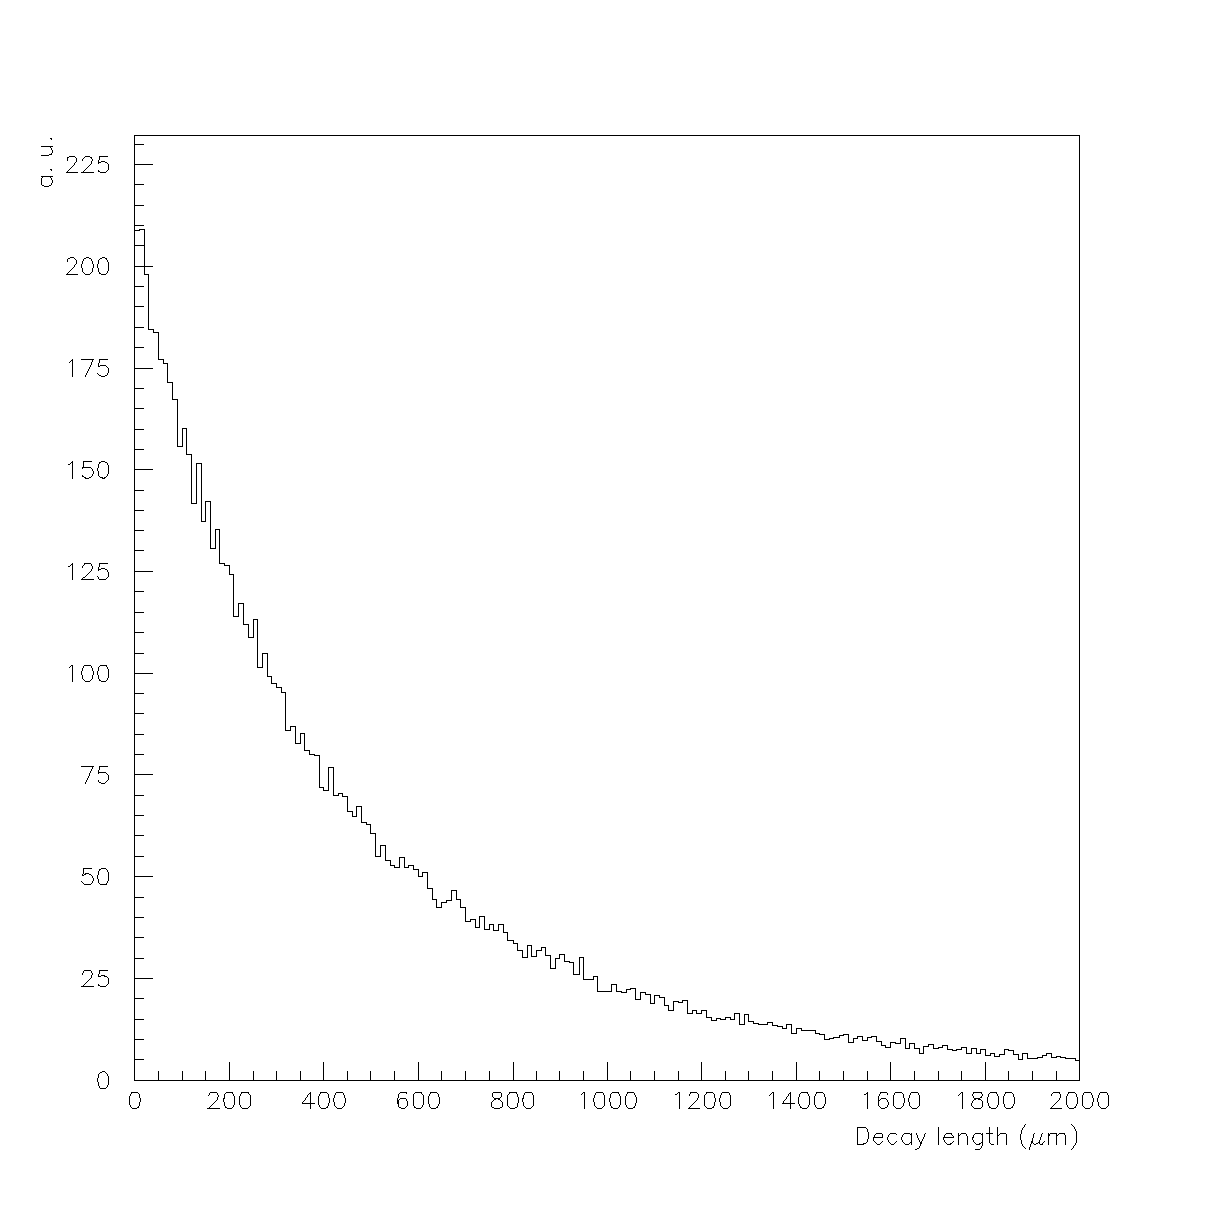
\includegraphics[width=95mm,height=95mm]{./figure_cap2/decadim_tau_CNGS.eps}
\end{center}
\caption{Distribuzione delle lunghezze di decadimento del $\protect\tau $
prevista nell'esperimento OPERA.}
\end{figure}
 
La struttura del rilevatore � stata quindi pensata allo scopo di
identificare la traccia del leptone $\tau$ e i due vertici che segnano
la sua produzione e il suo decadimento: il primario e un secondario
corrispondente al decadimento di tale particella, mediante l'uso di
emulsioni nucleari. Al contempo, data l'esiguita' del flusso di
neutrini a grande distanza dalla sorgente, il rivelatore deve avere
una grande massa, dell'ordine di grandezza delle migliaia di
tonnellate.  Viene quindi fatto ricorso alla tecnica della Emulsion
Cloud Chamber (ECC), introdotta nel 1952 \cite{ECC} . Essa fu
successivamente sviluppata soprattutto in Giappone e utilizzata in
vari esperimenti. Di particolare rilevanza per la ricerca di
oscillazioni $\nu_\mu \rightarrow \nu_\tau$ e' la sua utilizzazione
per l'osservazione di neutrini tau da parte dell'esperimento DONUT
\cite{Donut}.

La tecnica ECC e' basata sull'uso delle emulsioni nucleari per il
tracciamento ad altissima risoluzione spaziale, mentre la massa del
rivelatore viene essenzialmente fornita da lastre di materiale passivo
inframmezzate ai fogli di emulsione nucleare. L'esperimento OPERA
utilizza un bersaglio segmentato, costituito da lastre di piombo
spesse 1 mm (che funge da materiale passivo) alternate a fogli di
emulsioni nucleari. Tale struttura consente la rivelazione diretta del
decadimento del $\tau $, prodotto nella interazione di corrente carica
(CC) dei $\nu _{\tau }$ nel bersaglio :
\begin{equation}
\nu _{\tau }N\rightarrow \tau ^{-}X  \tag{2.3}
\end{equation}

Le interazioni di CC del $\nu _{\tau }$ vengono cosi' identificate
dalla rivelazione del leptone $\tau $ tramite l'osservazione delle sue tipologie di
decadimento e, in particolare, in quelle a singola traccia carica (\emph{single-prong}) 
ossia in un elettrone, un muone o un adrone:
\begin{eqnarray*}
\tau ^{-} &\rightarrow &e^{-}\nu _{\tau }\overline{\nu }_{e} \\
\tau ^{-} &\rightarrow &\mu ^{-}\nu _{\tau }\overline{\nu }_{\mu } \\
\tau ^{-} &\rightarrow &h^{-}\nu _{\tau }(n\pi ^{0})
\end{eqnarray*}

I rapporti di decadimento sono: $17.8\%$ per il canale elettronico, $%
17.4\%$ per il canale muonico e $49.5\%$ per quello adronico con singolo
adrone carico.
Il restante 15.2\% si riferisce al decadimento a tripla traccia carica (%
\emph{multi-prong}): $\tau ^{-}\rightarrow \pi ^{+}\pi ^{-}\pi ^{-}\nu
_{\tau }(n\pi ^{0})$.

I decadimenti a singola traccia carica sono caratterizzati da una configurazione a
 \emph{gomito}, ove la traccia del $\tau $ stesso e quella del suo prodotto di decadimento
carico formano un angolo comunenemente detto \emph{angolo di kink}, come mostrato in figura 2.6.
 La identificazione  dell'evento, in base all'angolo di kink, avviene
grazie all'altissima risoluzione delle emulsioni nucleari.

\begin{figure}[tbp]
\begin{center}
 \includegraphics[height=6cm,width=8cm,angle=270]{./figure_cap2/figura2_4.eps}
\end{center}
\caption{Interazione di corrente carica del $\protect\nu _{\protect\tau }$ con
il successivo tipico decadimento a gomito del $\protect\tau $ in una singola particella carica}.
\end{figure}

L'area totale di emulsioni necessarie necessaria per OPERA \`{e} elevatissima, dell'ordine
 di $\sim 10^{5}$ $m^{2}$. La realizzazione dell'esperimento \`{e} quindi strettamente legata 
allo sviluppo di tecniche di produzione industriale su larga scala di emulsioni nucleari. 
Essa dipende anche strettamente dallo straordinario progresso delle tecniche di 
scansione automatica che sta avendo luogo in questi anni.

La presa dati di OPERA avr\`{a} inizio nel 2006


\section{L'apparato sperimentale}
\subsection{La cella ECC}

Il rivelatore utilizzato dall'esperimento OPERA \cite{B6} presenta una struttura
altamente modulare. Una cella della struttura a ECC \`{e} costituita da una 
lastra di materiale passivo
seguita da un sottile foglio di emulsione nucleare (\emph{ES}, \emph{%
Emulsion Sheet}). Nel caso di OPERA, la lastra di materiale passivo \`{e} una
lamina di piombo spessa $1$ $mm$, mentre il foglio di emulsione \`{e}
ottenuto fissando $\sim 45$ $\mu m$ di gel su entrambe le facce di un
supporto di plastica (\emph{base}) spesso $\sim 200$ $\mu m$ (figura 2.7).

L'alta densit\`{a} del piombo permette di ottenere un rivelatore di grande massa con
una minima distanza tra i fogli di emulsione. Vengono cos\`{i} minimizzati i decadimenti del 
$\protect\tau$ nella stessa lastra di materiale passivo in cui esso \`{e} prodotto, pi\`{u}
difficili da identificare. Inoltre l'alto Z e quindi la bassa lunghezza di radiazione del piombo
(Xo = 5,6 mm)  consentono la misura della quantit\`{a} di moto per diffusione multipla coulombiana, 
nonch\'{e} l'identificazione degli elettroni e la misura della loro energia
tramite l'osservazione degli sciami elettromagnetici da essi generati. La
radioattivit\`{a} naturale residua del piombo va tuttavia tenuta sotto controllo, al fine di 
evitare che le emulsioni vengano impressionate da tracce di fondo
(\emph{background}).

\begin{figure}[tbp]
\begin{center}
\includegraphics[width=110mm,height=60mm]{./figure_cap2/figura2_6.eps}
\end{center}
\caption[Struttura schematica di una cella ECC.]{Struttura schematica di una
cella ECC; nel caso, rappresentato in figura, in cui il $\protect\tau $ decade a valle della
 lastra di piombo in cui 
\`{e} stato prodotto, l'angolo di kink viene ricostruito tramite i quattro segmenti di
traccia nei films di emulsione.}
\end{figure}

Le emulsioni sono costituite da bromuro di argento immerso in una gelatina. Una volta che esse 
sono sviluppate, il passaggio di una particella carica \`{e} indicato da una serie di \emph{grani}
 di colore scuro. Le emulsioni nucleari sono caratterizzate da una sensibilit\`{a} a \emph{singole}
particelle e dalle costanti e piccole dimensione dei grani, dell'ordine del micron, in modo tale da 
assicurare una elevata risoluzione spaziale.

Il numero di grani anneriti che si formano in $\sim 45$ $\mu m$ di emulsione
 \`{e} dell'ordine di 15 e quindi sufficiente per la ricostruzione di
 \emph{micro-tracce}, anche mediante tecniche di \emph{scansione automatica}.

Il passaggio di una particella carica attraverso una cella ECC genera quindi
un segmento di traccia, o micro-traccia, in ciascuno degli strati di emulsione
da una parte e dall'altra della base di plastica. Connettendo i grani che nelle
due micro-tracce sono prossimi alla base, si ottiene una \emph{traccia di base}. Essa
 consente di ricostruire la traccia della particella con una migliore risoluzione angolare 
(dell'ordine di qualche milliradiante o ancora meglio in caso di misure di precisione)
dato che i grani prossimi alla base di plastica non sono affetti dalle, seppur piccole, 
distorsioni negli strati di emulsione indotte dal processo di sviluppo.

Nel 40\% dei casi, il $\tau $ decade nelle emulsioni o all'interno della
lastra di piombo immediatamente a valle rispetto a quella in cui \`{e}
avvenuta l'interazione primaria del $\nu _{\tau }$; si parla, allora, di 
\emph{decadimento lungo}. Nel restante 60\% dei casi, invece, esso decade entro la
stessa lastra del vertice di interazione (\emph{decadimento corto}).

Nel primo caso, il $\tau $ viene rivelato misurando l'angolo di kink formato
dalla direzione\ della traccia di base lasciata dal $\tau $ stesso e dalla
direzione della traccia di base generata dalla particella prodotta nel
decadimento (figura 2.7). La traccia del $\tau $ si trova nel foglio
d'emulsione che precede la lastra di piombo in cui si \`{e} verificato il
decadimento, mentre la traccia della particella prodotta \`{e} individuata
nel foglio immediatamente sucessivo.

Per i decadimenti corti si adotta, invece, il metodo del \emph{parametro di
impatto} (\emph{IP}). Si localizza anzitutto il vertice di interazione, mediante almeno due tracce.
Un evento \`{e} considerato \emph{candidato} se un'altra traccia, estrapolata all'indietro, ha 
una minima distanza dal vertice, ossia parametro di impatto, superiore ad un valore di soglia 
dipendente dalla posizione longitudinale del vertice ricostruito. Questi eventi presentano un
 rapporto segnale/rumore meno favorevole rispetto a quelli in cui il $\tau $ subisce
un decadimento lungo.

\subsection{La struttura del rivelatore}

In figura 2.8 \`{e} riportata la struttura modulare dell'apparato
sperimentale nella sua attuale configurazione. L'unit\`{a} fondamentale
della struttura \`{e} detta \emph{mattone} (o \emph{brick}) ed \`{e}
costituita da una sequenza in cui lastre di piombo si alternano a fogli di
emulsione, per un totale di 56 celle ECC. L'uso di mattoni consente di
costruire un \emph{bersaglio attivo} altamente modulare e sufficientemente compatto,
con una massa complessiva di $\sim 1.8$ $kt$.

\begin{figure}[tbp]
\begin{center}
\includegraphics{./figure_cap2/figura2_7.eps}
\end{center}
\caption[Schema del rivelatore di OPERA nella sua attuale configurazione.]{%
Schema del rivelatore di OPERA nella sua attuale configurazione. Sono
visibili i moduli del bersaglio e la loro struttura di supporto, 
 fissata alla parte superiore dei due spettrometri per muoni a ferro magnetizzato.}
\end{figure}

Ciascun mattone presenta dimensioni trasverse pari a $(10.2\times 12.7)$ $%
cm^{2}$ che sono frutto di una scelta di compromesso. Una volta avvenuta
l'interazione, infatti, il mattone viene rimosso e le emulsioni vengono
analizzate; la massa del singolo mattone deve garantire la possibilit\`{a} di
poterlo rimuovere con la minima perdita di massa del rivelatore.
Inoltre, l'estrazione di mattoni aventi piccole dimensioni risulta
meccanicamente pi\`{u} semplice.
 D'altra parte, mattoni di dimensioni eccessivamente piccole accentuano
gli effetti di bordo. In tabella 2.2 sono riportate le principali
caratteristiche di un mattone.

\begin{table}[tbp]
\centering
\begin{tabular}{||c|c||}
\hline\hline
Spessore singola cella ECC ($mm$) & $1.3$ \\ \hline
Numero di celle/mattone & $56$ \\ \hline
Numero di fogli di emulsione/mattone & $58$ \\ \hline
Dimensioni trasversali ($cm^{2}$) & $10.2\times 12.7$ \\ \hline
Dimensioni longitudinali ($cm$) & $7.5$ \\ \hline
Dimensioni longitudinali ($X_{0}$) & $10$ \\ \hline
Peso ($Kg$) & $7.9(Pb)+0.4(emulsioni)$ \\ \hline\hline
\end{tabular}
\caption{Caratteristiche di un mattone.}
\end{table}

Grazie alla sua struttura e alle sue dimensioni (figura 2.9), il mattone permette di misurare la 
quantit\`{a} di moto delle particelle tramite la diffusione multipla coulombiana e di
discriminare elettroni da adroni mediante la rivelazione dello sciame
elettromagnetico prodotto nell'attraversamento delle lastre di piombo. Dato il loro grande numero,
i mattoni verranno costruiti da una macchina automatica specialmente progettata,
 detta \emph{Brick Assembly Machine} (BAM).

\begin{figure}[tbp]
\begin{center}
\includegraphics[width=100mm,height=80mm]{./figure_cap2/brick.eps}
\end{center}
\caption{Struttura schematica di un mattone di OPERA.}
\end{figure}

I mattoni sono assemblati in maniera da formare \emph{muri} (o \emph{walls})
verticali da 3328 mattoni (52 in orizzontale $\times $ 64 in verticale), ortogonali alla direzione
del fascio. Le dimensioni complessive di un muro sono $6.7\times 6.7$ $m^{2}$ e la sua massa \`{e}
 $27$ $ton$. La struttura di supporto di un muro (figura
2.10) consta di bande verticali e guide orizzontali sui quali i mattoni
sono posizionati entro una precisione di $1$ $mm$. Essa \`{e} estremamente
leggera ($\sim 0.4\%$ della massa complessiva del bersaglio), essendo stata
progettata con l'obiettivo di minimizzare il numero di interazioni da
neutrino che avvengono in essa e non nei mattoni. Il caricamento dei mattoni nella
struttura in fase di installazione dell'esperimento e la loro estrazione in seguito
a interazioni di neutrini  vengono attuati
tramite un sistema automatico denominato \emph{Brick Manipulator System} (BMS).

\begin{figure}[tbp]
\begin{center}
\includegraphics[width=80mm,height=95mm]{./figure_cap2/figura2_8.eps}
\end{center}
\caption{Struttura di supporto per un muro del rivelatore di OPERA.}
\end{figure}
Ogni muro di mattoni � seguito da due piani di tracciamento elettronici (\emph{Target
Trackers}, \emph{TT}). Questi piani sono realizzati 
mediante \emph{strips} di scintillatore plastico ($2.6$ $cm\times 1$ $cm\times 6.7$ $m$) e
 contengono ciascuno 256 strips. Ogni gruppo di 64 strips costituisce una unit� indipendente 
letta mediante un fotorivelatore a 64-pixels, cosicch\`{e} ogni piano viene letto 
da 8 fotorivelatori. Le strips del \emph{TT} sono larghe 2.6 $cm$ e spesse 1 $cm$.
Vengono abbinati due piani di TT con strips orientate lungo X e rispettivamente lungo Y. Simulazioni 
Monte Carlo hanno confermato che la segmentazione adottata non abbassa eccessivamente
 l'efficienza per l'identificazione del mattone in cui \`{e} avvenuta l'interazione, il 
che costituisce il compito primario del TT. La regolare rimozione dei mattoni indicati dal TT
permette una analisi \emph{quasi-online} delle emulsioni e, dunque, degli eventi di interazione.

Un muro interfacciato da due piani di tracciamento TT costituisce un \emph{modulo} del
rivelatore. Una sequenza di 31 moduli, seguita da uno spettrometro per muoni, definisce
un \emph{supermodulo}.

Lo spettrometro per muoni costituisce la parte finale di ciascun supermodulo. 
Il suo scopo � l'identificazione dei muoni e la misura della loro carica e quantit� di moto. Esso
consta di un magnete dipolare composto da due muri di ferro magnetizzato ($%
B=1.55$ $T$) alternati a coppie di piani di tubi a drift (\emph{Precision
Trackers, PT}). Ogni muro \`{e} segmentato in 12 piani di lastre di ferro, tra i
quali sono collocati piani di \emph{Resistive Plate Chambers} (\emph{RPC})
per il tracciamento e l'identificazione dei muoni, assieme al TT e al PT. 

Lo spettrometro permette di ridurre 
il fondo dovuto alla produzione di charm, il quale � proporzionale alla inefficienza 
nell'identificazione del muone primario \cite{charm}. Lo spettrometro permette anche 
di misurare la carica del muone e quindi di ridurre ulteriormente il fondo dovuto
 ai $\mu^+$ dovuti al decadimento di una particella con charm prodotta nella interazione 
primaria. La produzione di charm avviene in interazioni sia di CC che di NC attraverso 
le reazioni:
\begin{eqnarray}
\nu_\mu N\rightarrow c \mu X\\
\nu_\mu N \rightarrow c \bar{c} \mu X\\
\nu_\mu N\rightarrow c\bar{c}\nu_\mu X
\end{eqnarray}
Le particelle con charm hanno una massa e una vita media simili a quelle del $\tau$. 
Pertanto possono simulare un evento di $\tau$, sopratutto se il $\mu$ o l'altra particella 
charmata non vengono identificati.


\subsection{Localizzazione del mattone}

La ricostruzione dell'evento fornita dai rivelatori elettronici permette di
identificare, in tempo reale, il mattone in cui si \`{e} verificata
l'interazione da neutrino.

L'efficienza con cui avviene la localizzazione del mattone dipende
sostanzialmente da due fattori:
\begin{itemize}
\item  in primo luogo, dall'identificazione del muro;
\item  in secondo luogo, dall'individuazione del mattone all'interno del
muro suddetto.
\end{itemize}

Nel processo di rilevamento del muro, gioca un ruolo determinante il 
\emph{backscattering}, ossia la diffusione di particelle secondarie in
direzione opposta rispetto a quella del fascio di neutrini. Esso, infatti,
pu\`{o} determinare un segnale spurio in uno o pi\`{u} piani di
tracciamento, appartenenti a moduli posti a monte del muro-bersaglio. In
tabella 2.3 \`{e} riportata l'efficienza di identificazione del muro, che
risulta essere compresa tra l'87\% ed il 96\%.

\begin{table}[tbp]
\centering
\begin{tabular}{||c|c||}
\hline\hline
\textbf{Tipologia dell'evento} & \textbf{Efficienza} \\ \hline
DIS $\nu _{\mu }$ CC & $90.2\%$ \\ \hline
DIS $\nu _{\mu }$ NC & $86.6\%$ \\ \hline
DIS $\tau \rightarrow \mu $ & $90.7\%$ \\ \hline
DIS $\tau \rightarrow e$ & $92.9\%$ \\ \hline
QE $\nu _{\mu }$ CC & $89.7\%$ \\ \hline
QE $\tau \rightarrow \mu $ & $92.9\%$ \\ \hline
QE $\tau \rightarrow e$ & $95.9\%$ \\ \hline\hline
\end{tabular}
\caption[Efficienza di identificazione del \emph{muro}, calcolata per
interazioni di $\protect\nu _{\protect\mu }$ e di $\protect\nu _{\protect\tau
}$ altamente inelastiche (DIS) e quasi-elastiche (QE).]{Efficienza di
identificazione del \emph{muro}, calcolata per interazioni di $\protect\nu _{%
\protect\mu }$ e di $\protect\nu _{\protect\tau }$ profondamente inelastiche
(DIS) e quasi-elastiche (QE). Gli eventi di $\protect\nu _{\protect\tau }$
sono classificati in base al canale di decadimento del $\protect\tau $.}
\end{table}

Una volta identificata il muro, si procede alla individuazione
del mattone all'interno del muro, usufruendo delle informazioni provenienti dai
corrispondenti piani di tracciamento. L'efficienza di identificazione del mattone in cui 
\`{e} avvenuta l'interazione \`{e} fornita nella tabella 2.4, in funzione del numero di mattoni 
rimossi per ciascun evento. Essa \`{e} limitata dalla risoluzione spaziale dei rivelatori di
tracciamento. Nell'ipotesi in cui venga rimosso dal bersaglio un solo mattone
per evento, l'efficienza varia tra il 67\% e l'84\%.

\begin{table}[tbp]
\begin{center}
\begin{tabular}{|c|c|c|c|}
\hline
\textbf{Tipologia dell'evento} & \textbf{1 mattone rimosso} & \textbf{2 mattoni
rimossi} & \textbf{3 mattoni rimossi} \\ \hline
DIS $\nu _{\mu }$ CC & 78.3\% & 86.2\% & 92.2\% \\ \hline
DIS $\nu _{\mu }$ NC & 66.7\% & 77.6\% & 79.6\% \\ \hline
DIS $\tau \rightarrow \mu $ & 74.6\% & 84.6\% & 89.2\% \\ \hline
DIS $\tau \rightarrow e$ & 81.8\% & 89.4\% & 90.5\% \\ \hline
QE $\nu _{\mu }$ CC & 81.7\% & 91.5\% & 95.4\% \\ \hline
QE $\tau \rightarrow \mu $ & 75.2\% & 83.5\% & 91.2\% \\ \hline
QE $\tau \rightarrow e$ & 83.9\% & 92.6\% & 93.2\% \\ \hline
\end{tabular}
\caption[Efficienza di identificazione del \emph{mattone}, determinata per
interazioni di $\protect\nu _{\protect\mu }$ e di $\protect\nu _{\protect\tau
}$ altamente inelastiche (DIS) e quasi-elastiche (QE), in funzione del
numero di mattoni rimossi per evento.]{Efficienza di identificazione del \emph{%
mattone}, determinata per interazioni di $\protect\nu _{\protect\mu }$ e di $%
\protect\nu _{\protect\tau }$ profondamente inelastiche (DIS) e quasi-elastiche
(QE), in funzione del numero di mattoni rimossi per evento. Gli eventi di $%
\protect\nu _{\protect\tau }$ sono classificati in base al canale di
decadimento del $\protect\tau $. I valori sono comprensivi del contributo di
identificazione del muro.}
\end{center}
\end{table}

I valori di efficienza mostrati nelle tabelle 2.3 e 2.4 si riferiscono
all'analisi descritta nella proposta dell'esperimento. Una serie di studi
successivi, finalizzati ad una valutazione pi\`{u} accurata del
backscattering, hanno indicato una riduzione di $\sim 10\%$ dell'efficienza
complessiva di localizzazione del mattone.

Si calcola che, a intensit\`{a} nominale del fascio, avverranno circa 30 interazioni
 di neutrino al giorno.
Per ogni segnale di \emph{trigger}, in base alla predizione dei rivelatori
di tracciamento, verr\`{a} estratto dal bersaglio il mattone corrispondente.

\subsection{I Changeable Sheets}

I \textbf{C}\emph{hangeable} \textbf{S}\emph{heets} (\textbf{CS})
rappresentano un elemento importante nella configurazione del rivelatore di
OPERA. Essi sono stati introdotti, dopo la presentazione della proposta di esperimento,
 per ridurre la superficie totale di
emulsione da sottoporre al processo di scansione e migliorare sensibilmente,
nel contempo, l'efficienza di localizzazione del mattone. In questo lavoro di tesi 
\`{e} stato condotto un primo studio sperimentale della loro efficacia. 

Un CS \`{e} un foglio di emulsione che funge da interfaccia tra il mattone ed
il piano di tracciamento TT immediatamente a valle. 

Il CS viene impacchettato separatamente dal mattone ed incollato ad
esso utilizzando un adattatore la cui forma scaturisce dalla
necessit\`{a} di assicurare il parallelismo tra CS e mattone entro
$20$ $mrad$.

L'analisi del CS relativo a ciascun mattone rimosso dal bersaglio ha lo scopo
di individuare tracce associate all'evento. Nel caso in cui tale ricerca
abbia esito negativo, il mattone, ancora impacchettato, viene dotato di un
nuovo CS e pu\`{o} essere riutilizzato (non necessariamente nella stessa
posizione). Viene quindi estratto, tra i mattoni adiacenti al suddetto o
appartenenti al muro immediatamente a valle, quello con la pi\`{u} alta
probabilit\`{a} di contenere l'evento. In tal modo, si stima che
l'efficienza di localizzazione del mattone aumenti fino a $\sim 90\%$
(rispetto al $70\%\div 80\%$ attuale).

L'inserimento del CS, tuttavia, comporta una piccola riduzione di efficienza
($\sim 0.2\%$) nella rivelazione dei $\tau $ prodotti nelle interazioni di $%
\nu $ all'interno della lastra di piombo pi\`{u} a valle tra quelle del mattone.

In base al tipo di evento (CC oppure NC), vengono adottate due differenti
strategie per la ricerca di tracce prodotte in interazioni di neutrino:

\begin{itemize}
\item  nel caso di eventi di corrente carica, viene effettuata la ricerca,
in un'area di $\sim 5\times 5$ $cm^{2}$ intorno alla posizione predetta, di
una traccia compatibile col muone identificato dai rivelatori elettronici,
entro una tolleranza angolare dell'ordine della risoluzione del TT ($\sim 20$
$mrad$);

\item  per quanto concerne gli eventi di corrente neutra, la qualit\`{a}
della ricostruzione dell'evento peggiora e, di conseguenza, l'area da
sottoporre a scansione \`{e} estesa a $\sim 10\times 10$ $cm^{2}$, coprendo
due o pi\`{u} mattoni. Nell'ipotesi di assenza di predizioni, si procede col
ricercare in emulsione particelle con un angolo entro l'accettanza massima,
pari a $400$ $mrad$.
\end{itemize}

La densit\`{a} di tracce di fondo registrate nel CS rappresenta un parametro
critico sia per la riduzione del tempo di scansione delle emulsioni che 
per una efficiente localizzazione del mattone, soprattutto per gli
eventi NC. I cosmici accumulati dalla produzione fino alla fase di
assemblaggio del mattone (nonch\'{e} durante l'esperimento), la
radioattivit\`{a} ambientale e le interazioni di neutrino che avvengono
nella roccia intorno al rivelatore e nel bersaglio a monte sono sorgenti di
fondo, il cui livello in emulsione deve essere valutato con attenzione e
ridotto al minimo possibile.

Per le emulsioni di OPERA \`{e} stato ideato un metodo, denominato \emph{refreshing}, per
''cancellare'' una frazione significativa di tracce registrate in emulsione.
Il procedimento sar\`{a} applicato a tutti i fogli prima del loro trasporto
al Gran Sasso e consiste nel mantenere le emulsioni, per tre giorni, ad una
temperatura di $30$ $%
%TCIMACRO{\UNICODE[m]{0xb0}}%
%BeginExpansion
{{}^\circ}%
%EndExpansion
C$ ed un'umidit\`{a} relativa del $\sim 98\%$. Per i CS,
\`{e} prevista un'ulteriore fase di refreshing appena prima
dell'impacchettamento per l'esposizione, al fine di sopprimere il fondo
 dovuto ai cosmici accumulati durante il trasporto.
D'altra parte, alcune prove preliminari indicano che, impacchettando i CS in
modo stagno ad
una umidit\`{a} del 90\%, \`{e} ragionevole assumere che, nell'arco di tempo
in cui i fogli saranno conservati al Gran Sasso prima dell'installazione, ad
una temperatura non superiore a $20$ $%
%TCIMACRO{\UNICODE[m]{0xb0}}%
%BeginExpansion
{{}^\circ}%
%EndExpansion
C$, il fondo iniziale possa essere cancellato per \emph{auto-refreshing}. In
tal caso, il refreshing al Gran Sasso potrebbe essere evitato. In maniera
simile, l'auto-refreshing consentir\`{a} di eliminare le tracce di fondo
accumulate nel corso dell'esperimento.

\subsection{Localizzazione e selezione di una interazione di $\protect\nu $
nel mattone}

L'analisi degli eventi in emulsione richiede che i fogli di un mattone siano
intercalibrati con una precisione dell'ordine del $\mu m$. Per conseguire
questo livello di accuratezza, occorre disporre di tracce di riferimento che
attraversino l'intero mattone con una densit\`{a} di $2\div 3/mm^{2}$.
Considerata la bassa densit\`{a} di tracce collegate al fascio di neutrini,
 si rende necessaria l'esposizione dei mattoni ad un flusso controllato
di cosmici, la cui durata e modalit\`{a} sono in fase di studio accurato con
una serie di prove effettuate al Gran Sasso. Dopo l'esposizione ai
cosmici, il mattone viene disassemblato e si procede allo sviluppo dei fogli
di emulsione.

La fase successiva consiste nella localizzazione della interazione di
$\nu $. Utilizzando le tracce misurate nel CS come predizioni, si
effettua, per ognuna di esse, una ricerca a ritroso nel mattone
(\emph{scan-back}), emulsione dopo emulsione, fino all'eventuale punto
della loro scomparsa. Una traccia che non sia stata trovata in tre
fogli consecutivi costituisce un \emph{segnale di vertice} ed il
primo piatto in cui tale traccia non \'e trovata viene definito piatto
del vertice. I motivi per cui una traccia pu\'o non essere trovata
sono tre: la traccia di {\emph scan-back} pu\'o avere origine da un
vertice primario di interazione di neutrino; la traccia di {\emph
scan-back} pu\'o portare ad un vertice secondario; la traccia pu\'o
essere presente nei piatti pi\'u a monte ma non \'e trovata a causa
delle inefficienze. Lo scopo della successiva analisi al vertice \'e
di distinguere tra questi casi. A tal scopo viene definito un volume
attorno al piatto del vertice (ossia un'area di $5\times 5$ $mm^{2}$
per 8 fogli) e si effettua la ricerca di tutte le altre tracce associate
all'evento. Si individuano due diverse topologie di vertice:

\begin{itemize}
\item  vertici originati da una particella  \emph{ carica}

\item  vertici originati da una particella \emph{neutra}

\end{itemize}

Il primo caso corrisponde ad una topologia di vertice secondario, in
tal caso la traccia madre carica \'e, a sua volta, inseguita a ritroso
per risalire al vertice di interazione primario. Nel secondo caso si
\'e in presenza o della interazione primaria di neutrino, oppure di un
decadimento secondario di particelle charmate neutre o di una
interazione secondaria indotta da un neutrone. Una volta che entrambi
i vertici, primario e secondario, sono stati individuati l'evento
candidato \'e sottoposto ad una dettagliata analisi topologica e
cinematica.


\section{Prestazioni dell'esperimento}

Nel paragrafo 2.3, si \`{e} visto che il segnale di oscillazione $\nu _{\mu
}\rightarrow \nu _{\tau }$ consiste nella rivelazione del $\tau ^{-}$
prodotto nel processo di corrente carica (2.3) attraverso la caratteristica
topologia di decadimento (\emph{kink}) nei canali elettronico, muonico e in
singolo adrone carico. Si \`{e} poi distinto il decadimento in \emph{corto}
o \emph{lungo} a seconda del fatto che esso abbia luogo nella medesima
lastra di piombo in cui avviene l'interazione primaria da $\nu $ o nella
lastra immediatamente a valle.

In tabella 2.5 \`{e} riportato, per ciascuno dei canali di decadimento del $%
\tau $, il numero di eventi di segnale attesi in cinque anni di presa-dati ($%
2.25\times 10^{20}$ $pot$), per tre differenti valori di $\Delta m^{2}$ e
nell'ipotesi di mescolamento massimale. Sono altres\`{\i} mostrati gli eventi di
fondo attesi.

\begin{table}[tbp]
\centering
\begin{tabular}{||c|c|c|c|c||}
\hline\hline
\textbf{Canale di decadimento} & \textbf{Segnale (1)} & \textbf{Segnale (2)}
& \textbf{Segnale (3)} & \textbf{Fondo} \\ \hline
$\tau \rightarrow e$ $lungo$ & $1.4$ & $3.4$ & $8.6$ & $0.15$ \\ \hline
$\tau \rightarrow \mu $ $lungo$ & $1.3$ & $3.2$ & $8.1$ & $0.29$ \\ \hline
$\tau \rightarrow h$ $lungo$ & $1.6$ & $3.7$ & $9.4$ & $0.23$ \\ \hline
$\tau \rightarrow e$ $corto$ & $0.4$ & $1.0$ & $2.5$ & $0.03$ \\ \hline
$\tau \rightarrow \mu $ $corto$ & $0.2$ & $0.5$ & $1.3$ & $0.04$ \\ \hline
Totale & $4.9$ & $11.8$ & $29.9$ & $0.74$ \\ \hline\hline
\end{tabular}
\caption[Eventi di $\protect\nu _{\protect\tau }$ e di fondo attesi in 5
anni di presa dati per tre diversi valori di $\Delta m^{2}$.]{Eventi di $%
\protect\nu _{\protect\tau }$ e di fondo attesi in 5 anni di presa dati per
tre diversi valori di $\Delta m^{2}$: $(1)\Leftrightarrow \Delta
m^{2}=1.6\times 10^{-3}$ $eV^{2}$; $(2)\Leftrightarrow \Delta
m^{2}=2.5\times 10^{-3}$ $eV^{2}$; $(3)\Leftrightarrow \Delta
m^{2}=4.0\times 10^{-3}$ $eV^{2}$. Si assume un mescolamento massimale.}
\end{table}

Una delle principali sorgenti di fondo \`{e} rappresentata dalla produzione
di particelle con \emph{charm} nelle interazioni di corrente carica di $\nu
_{\mu }$ e successivo decadimento in elettrone, muone o adrone, nel caso in
cui il muone primario non sia identificato.

Le reinterazioni adroniche e la diffusione a grande angolo dei muoni nel
piombo sono ulteriori sorgenti di fondo per i canali adronico e,
rispettivamente, muonico.

Le efficienze di rivelazione sono riassunte in tabella 2.6. La figura 2.11
mostra la sensitivit\`{a} dell'esperimento OPERA all'oscillazione $\nu _{\mu
}\rightarrow \nu _{\tau }$. In cinque anni di presa-dati, esso sar\`{a} in
grado di esplorare tutta la regione dello spazio dei parametri indicata, al
90\% di C.L., dai dati di SuperKamiokande.

\begin{table}[tbp]
\centering
\begin{tabular}{||c|c||}
\hline\hline
\textbf{Canale di decadimento} & \textbf{Efficienza} \\ \hline
$\tau \rightarrow e$ & $3.4\%$ \\ \hline
$\tau \rightarrow \mu $ & $2.8\%$ \\ \hline
$\tau \rightarrow h$ & $2.9\%$ \\ \hline
Totale & $9.1\%$ \\ \hline\hline
\end{tabular}
\caption{Efficienze di rivelazione per i canali di decadimento del $\protect%
\tau $ studiati.}
\end{table}

\begin{figure}[tbp]
\begin{center}
\includegraphics[width=80mm,height=80mm]{./figure_cap2/sensitivitaOPERA.eps}
\end{center}
\caption{Curva di sensitivit\`{a} dell'esperimento OPERA al 90\% C.L. in 5
anni di esposizione al fascio CNGS.}
\end{figure}
La tabella 2.7 fornisce il numero di eventi di segnale e di fondo attesi 
con la configurazione finale dell'apparato sperimentale. Viene dato il numero di
eventi attesi con l'intensit\`{a} nominale del fascio CNGS, quello nel
caso in cui l'intensit\`{a} del fascio stesso venga incrementata di un
fattore 1.5 (come in linea di principio appare possibile) e quello corrispondente
 ad un eventuale ulteriore miglioramento che � stato prospettato.

\begin{table}[tbp]
\centering
\begin{tabular}{||c|c|c|c|c||}
\hline\hline
& \textbf{Segnale (1)} & \textbf{Segnale (2)} & \textbf{Segnale (3)} & 
\textbf{Fondo} \\ \hline
\textbf{Hall C} & $6.0$ & $11.5$ & $29.2$ & $0.71$ \\ \hline
\textbf{CNGS}$\times $\textbf{1.5} & $9.0$ & $17.2$ & $43.8$ & $1.06$ \\ 
\hline
\textbf{Ulteriore miglioramento} & $10.3$ & $19.8$ & $50.4$ & $0.67$ \\ 
\hline\hline
\end{tabular}
\caption[Numero di eventi attesi nella configurazione definitiva]{Numero di
eventi di segnale e di fondo attesi, per l'intensit\`{a} nominale del fascio,
nel caso in cui l'intensit\`{a} sia aumentata di un fattore $1.5$ e nel caso 
in cui sia possibile un ulteriore miglioramento. $(1)\Leftrightarrow \Delta
m^{2}=1.8\times 10^{-3}$ $eV^{2}$; $(2)\Leftrightarrow \Delta
m^{2}=2.5\times 10^{-3}$ $eV^{2}$; $(3)\Leftrightarrow \Delta
m^{2}=4.0\times 10^{-3}$ $eV^{2}$.}
\end{table}

Il successo di un esperimento di ricerca di eventi rari, quale \`{e}
OPERA, dipende largamente dalla riduzione del fondo. Attualmente, si
sta studiando la possibilit\`{a} di introdurre, nell'analisi degli
eventi candidati, un metodo di identificazione in emulsione dei muoni
di bassa energia, in gran parte non individuati dai rivelatori
elettronici. Questo permetterebbe di ridurre ulteriormente il fondo
derivante dalla produzione di particelle con charm nelle interazioni
CC di $\nu _{\mu }$. Tale metodo si basa sulla misura della perdita di
energia per ionizzazione in regime non relativistico in prossimit\`{a}
del punto di arresto della particella. Risultati preliminari indicano
che il fondo pu\`{o} essere ridotto da $1.06$ a $\sim 0.67$.
%\end{document}

\chapter{IL tracciamento nelle ECC}

\section{Le emulsioni nucleari}

Le emulsioni nucleari sono  un  rivelatore di particelle con una straordinaria risoluzione
 risoluzione spaziale  ($<1$ $\mu m$). Il loro utilizzo ha 
consentito di conseguire importanti  scoperte nel campo della fisica nucleare e delle particelle
elementari \cite{pione,beauty}. Tuttavia a causa  della grande lentezza e laboriosit\`{a} con
della scansione, le emulsioni furono utilizzate sempre meno. Con l' avvento
delle moderne e sofisticate tecniche di scansione automatica, sviluppate negli anni '80 ed per prime applicate con successo nell' esperimento CHORUS \cite{A29}, la tecnica delle emulsioni
ha conosciuto una vera e propria rinascita, determinandone cos\`{i}
l'applicazione su vasta scala come nell'esperimento OPERA.

Le emulsioni nucleari sono costituite da microcristalli di bromuro di
argento (AgBr) dispersi in uno strato gelatinoso di sostegno. Le
dimensioni dei microcristalli sono pari a circa $0.2$ $\mu m$ e la loro concentrazione in emulsione varia dal dal $25\%$ al $50\%$ in volume. La loro
realizzazione \`{e} accuratamente controllata grazie alla moderna tecnologia
industriale  sviluppata nel contesto dell'esperimento OPERA.

Le emulsioni presentano caratteristiche analoghe a quelle delle pellicole
fotografiche, ma con le seguenti differenze:

\begin{itemize}
\item  hanno uno spessore maggiore (da $50$ $\mu m$ a $\sim 1$ $mm$ rispetto
ai $5\div 10$ $\mu m$ delle pellicole);

\item  il loro contenuto di AgBr \`{e} superiore di un ordine di grandezza;

\item  i granuli di argento sviluppati hanno un diametro minore e risultano
pi\`{u} uniformi.
\end{itemize}

L'energia rilasciata dal passaggio di una particella carica o di un fotone
attraverso un'emulsione determina dei piccoli depositi di Ag metallico
principalmente sulla superficie del cristallo di AgBr coinvolto nel processo
(\emph{immagine latente}). L'interazione del campo elettrico della particella incidente con gli elettroni atomici o, nel caso dei fotoni, l'effetto fotoelettrico o Compton
provoca la ionizzazione di un cristallo di AgBr, creando atomi neutri di Br
e lacune positive $Ag^{+}$ e liberando elettroni che si portano in banda di
conduzione. Gli elettroni diffondono attraverso il cristallo finch\'{e} non
sono catturati da \emph{trappole}, presenti come imperfezioni del reticolo,
che acquistano carica negativa. Le trappole, ovvero impurit\`{a} aggiunte in
fase di produzione come agenti di sensibilizzazione, generano un campo
elettrico all'interno del cristallo e fungono da centri di cattura degli
ioni $Ag^{+}$ che, sotto l'influenza delle forze di Van der Waals, vengono
intrappolati e neutralizzati, trasformandosi in atomi di argento. 
In questo modo si formano aggregati di atomi di Ag (ossia {\emph{ immagini latenti}})
che agiscono da centri di sviluppo.

Le immagini latenti sono rese stabili da un complesso procedimento
fisico-chimico, che prende il nome di \emph{sviluppo}: introducendo
l'emulsione in una soluzione contenente agenti riducenti (principalmente
amidolo), altro argento viene indotto ad accumularsi attorno
all'Ag che ha dato luogo all'immagine latente; di conseguenza, il deposito
iniziale cresce fino alla creazione di \emph{grani scuri} disposti lungo la
traiettoria della particella.  La probabilit\`{a} che
questo processo si verifichi in cristalli che non hanno interagito con la
particella ionizzante \`{e} estremamente bassa. Tuttavia, un'alta
concentrazione di impurit\`{a} pu\`{o} dar luogo alla formazione di granuli
sparsi (che costituiscono un fondo ineliminabile) in genere dell'ordine di
qualche grano per $1000$ $\mu m^{3}$ di emulsione. I cristalli di AgBr non ridotti vengono disciolti mediante un bagno di fissaggio e, infine, lavati via dall'emulsione.

Le emulsioni nucleari forniscono un'immagine tridimensionale delle tracce,
che appaiono come sequenze di grani scuri, la cui posizione pu\`{o} essere
misurata con precisione sub-micrometrica. Da qui l'elevata
risoluzione spaziale di tali rivelatori.



\section{L'analisi delle emulsioni}

L'immagine tridimensionale immagazzinata nelle emulsioni viene acquisita
mediante un microscopio dotato di una telecamera CCD o CMOS e successivamente digitalizzata.
Algoritmi software gestiscono il riconoscimento dei grani, nonch\'{e} la
ricostruzione e la misura dei parametri delle tracce. Nel seguito descriviamo i principi di funzionamento di
dei sistemi discansione automatici sviluppati in Giappone e in Europa.


\subsection{Il sistema TS}
A partire dagli anni '80 \'{e} stato sviluppato in Giappone 
il sistema automatico  denominato \emph{Track Selector} (fig.\ref{fig:ts}). L'emulsione da analizzare \`{e} posizionata sul piatto di un
microscopio; essa viene ricoperta con campi del microscopio adiacenti
tramite successivi movimenti orizzontali del piatto. Il sistema acquisisce, all'interno delle emulsioni, una serie di \emph{immagini
tomografiche}, corrispondenti ad altrettanti livelli di messa a fuoco secondo la direzione verticale, su un
numero limitato di campi intorno alla posizione della traccia prevista. Il Track Selector ricostruisce le traccie sovrapponendo le immagini  con uno spostamento dei diversi strati determinato in base all'angolo  della traccia predetta dai rivelatori elettronici, la procedura � detta di Scan Back. Se non si ricerca una determinata traccia, ma tutte le traccie in un determinato intervallo angolare questa procedura viene ripetuta per un numero di volte fino  a coprire l'intera accettanza angolare richiesta. Questa seconda tipologia di scansione, detta NetScan,  � stata introdotta alla fine degli anni '90  grazie all'utilizzo di tecniche di processamento parallelo e un sistema  denominato  {\bf{U}}ltra {\bf{T}}rack {\bf{S}}elector (UTS). Per ogni traccia misurati i parametri  angololari e le posizioni.

\begin{figure}[tbp]
\begin{center}
\includegraphics[width=110mm,height=70mm]{./figure_cap2/TrackSelector.eps}
\end{center}
\caption{Principio di funzionamento del sistema Track Selector, sviluppato in Giappone.}
\label{fig:ts}
\end{figure}


In tabella \ref{table:ts} sono riportat i progessi dei sistemi di scansione automatica di emulsione a partire dal TS alle sue successive evoluzioni.

\begin{table}[tbp]
\begin{tabular}{||c|c|c|c|c||}
\hline\hline
\textbf{Sistema} & \textbf{Anno} & \textbf{V. scansione}$^{(1)}$ & \textbf{
V. scansione}$^{(2)}$ & \textbf{Esperimento} \\ \hline
TS & 1982 & 0.2 & non provato & CERN WA75/FNAL E653 \\ \hline
TS2 & 1994 & 0.4 & 0.008 & CHORUS \\ \hline
NTS & 1996 & 3 & 0.25 & CHORUS \\ \hline
UTS & 1998 & 3 & 3 & DONUT/CHORUS \\ \hline
S-UTS & 2005 & 30 & 30 & OPERA/DONUT \\ \hline\hline
\end{tabular}
\caption[Sviluppo delle caratteristiche dei sistemi di scansione delle
emulsioni nucleari.]{Sviluppo delle caratteristiche dei sistemi di scansione
delle emulsioni nucleari. La velocit\`{a} di scansione \`{e} espressa in
viste per secondo (una vista corrisponde ad un'area di $\sim 0.018$ $%
mm^{2}=150$ $\protect\mu m\times 120$ $\protect\mu m$). La velocit\`{a} (1)
si riferisce ad un angolo specifico, (2) a tutti gli angoli.}
\label{table:ts} 
\end{table}

Il sistema \textbf{S}\emph{uper} \textbf{UTS} (\textbf{S-UTS}) rappresenta
una ulteriore evoluzione del  Track Selector ed \`{e} stato
progettato e realizzato dall'Universit\`{a} di Nagoya (Giappone) per
raggiungere oltre $20~cm^2/h$ di velocit\'{a} di scansione necessari all'esperimento  OPERA. Il suo principio
di funzionamento \`{e} illustrato in fig.\ref{fig:sts}. L'acquisizione delle
immagini tomografiche dell'emulsione, con una telecamera CCD ad alte prestazioni (3KHz), avviene  senza interruzione del movimento dello stage grazie a un piezoelettrico che controlla il movimento verticale  dell'obiettivo sincronizzandolo con quello del tavolo. Ciascun campo di vista ($150\times 120$ $\mu m^{2}$) viene \emph{sezionato} in 16 livelli per la ricostruzione in 3D delle tracce. 

\begin{figure}[tbp]
\begin{center}
\includegraphics[width=90mm,height=90mm]{./figure_cap2/S-UTS.eps}
%\includegraphics{./figure_cap2/S-UTS.eps}
\end{center}
\caption{Principio di funzionamento del sistema S-UTS.}
\label{fig:sts}
\end{figure}


\section{Il sistema ESS}
Nei vari laboratori europei della collaborazione OPERA � stato sviluppato un sistema di scansione automatica, denominato ESS (European Scanning System), che utilizza per la ricostruzione delle traccie un approccio diverso dal TS. Tale approccio consiste nel realizzare una scansione tomografica dell'emulsione identificando tutti i grani di ciascun immagine: la ricostruzione della traccia, affidata ad un software dedicato, viene effettuata combinando grani appartenente a strati diversi. Tali combinazioni di grani definiscono traiettorie lungo le quali viene definito un volume di accettanza. Se il numero di grani all'interno di questo volume supera una soglia predefinita, la sequenza di grani costituisce una microtraccia. In tal modo ciascuna traccia viene ricostruita indipendentemente dal proprio angolo e  per questo motivo quest'approccio viene definito {\emph{multitraccia}}. 

Lo sviluppo dell'ESS  � basato sull'utilizzo di componenti hardware commerciali (o realizzata in collaborazione con industrie) in modo da poter trarre profitto dai continui sviluppi tecnologici del settore.   Il software utilizzato per la ricostruzione delle traccie, sviluppato in ambiente object-oriented, � realizzato secondo una struttura modulare che fornisce una flessibilit� tale da consentire successive modifiche hardware. La progettazione dell'ESS, tenendo conto dell'alta velocit� di scansione e di accuratezza in posizione ed angolo adeguate per l'analisi degli eventi, si � basata sulle seguenti linee guida:

\begin{itemize}
\item{utilizzo di meccanica di movimentazione ad alte prestazioni con precisioni di posizionamento sub-micrometrica;}
\item{ottica  con grande campo inquadrato;}
\item{telecamera con sensore CMOS ad alta risoluzione e frame rate;}
\item{potenti schede per il processamento delle immagini.}
\end{itemize}

In fig.\ref{fig:mic2} � mostrato il sistema (ESS) per l'analisi delle traccie in emulsione , mentre in figura \ref{fig:mic_schema} � riportato lo schema di principio. 


\begin{figure}[tbp]
\begin{center}
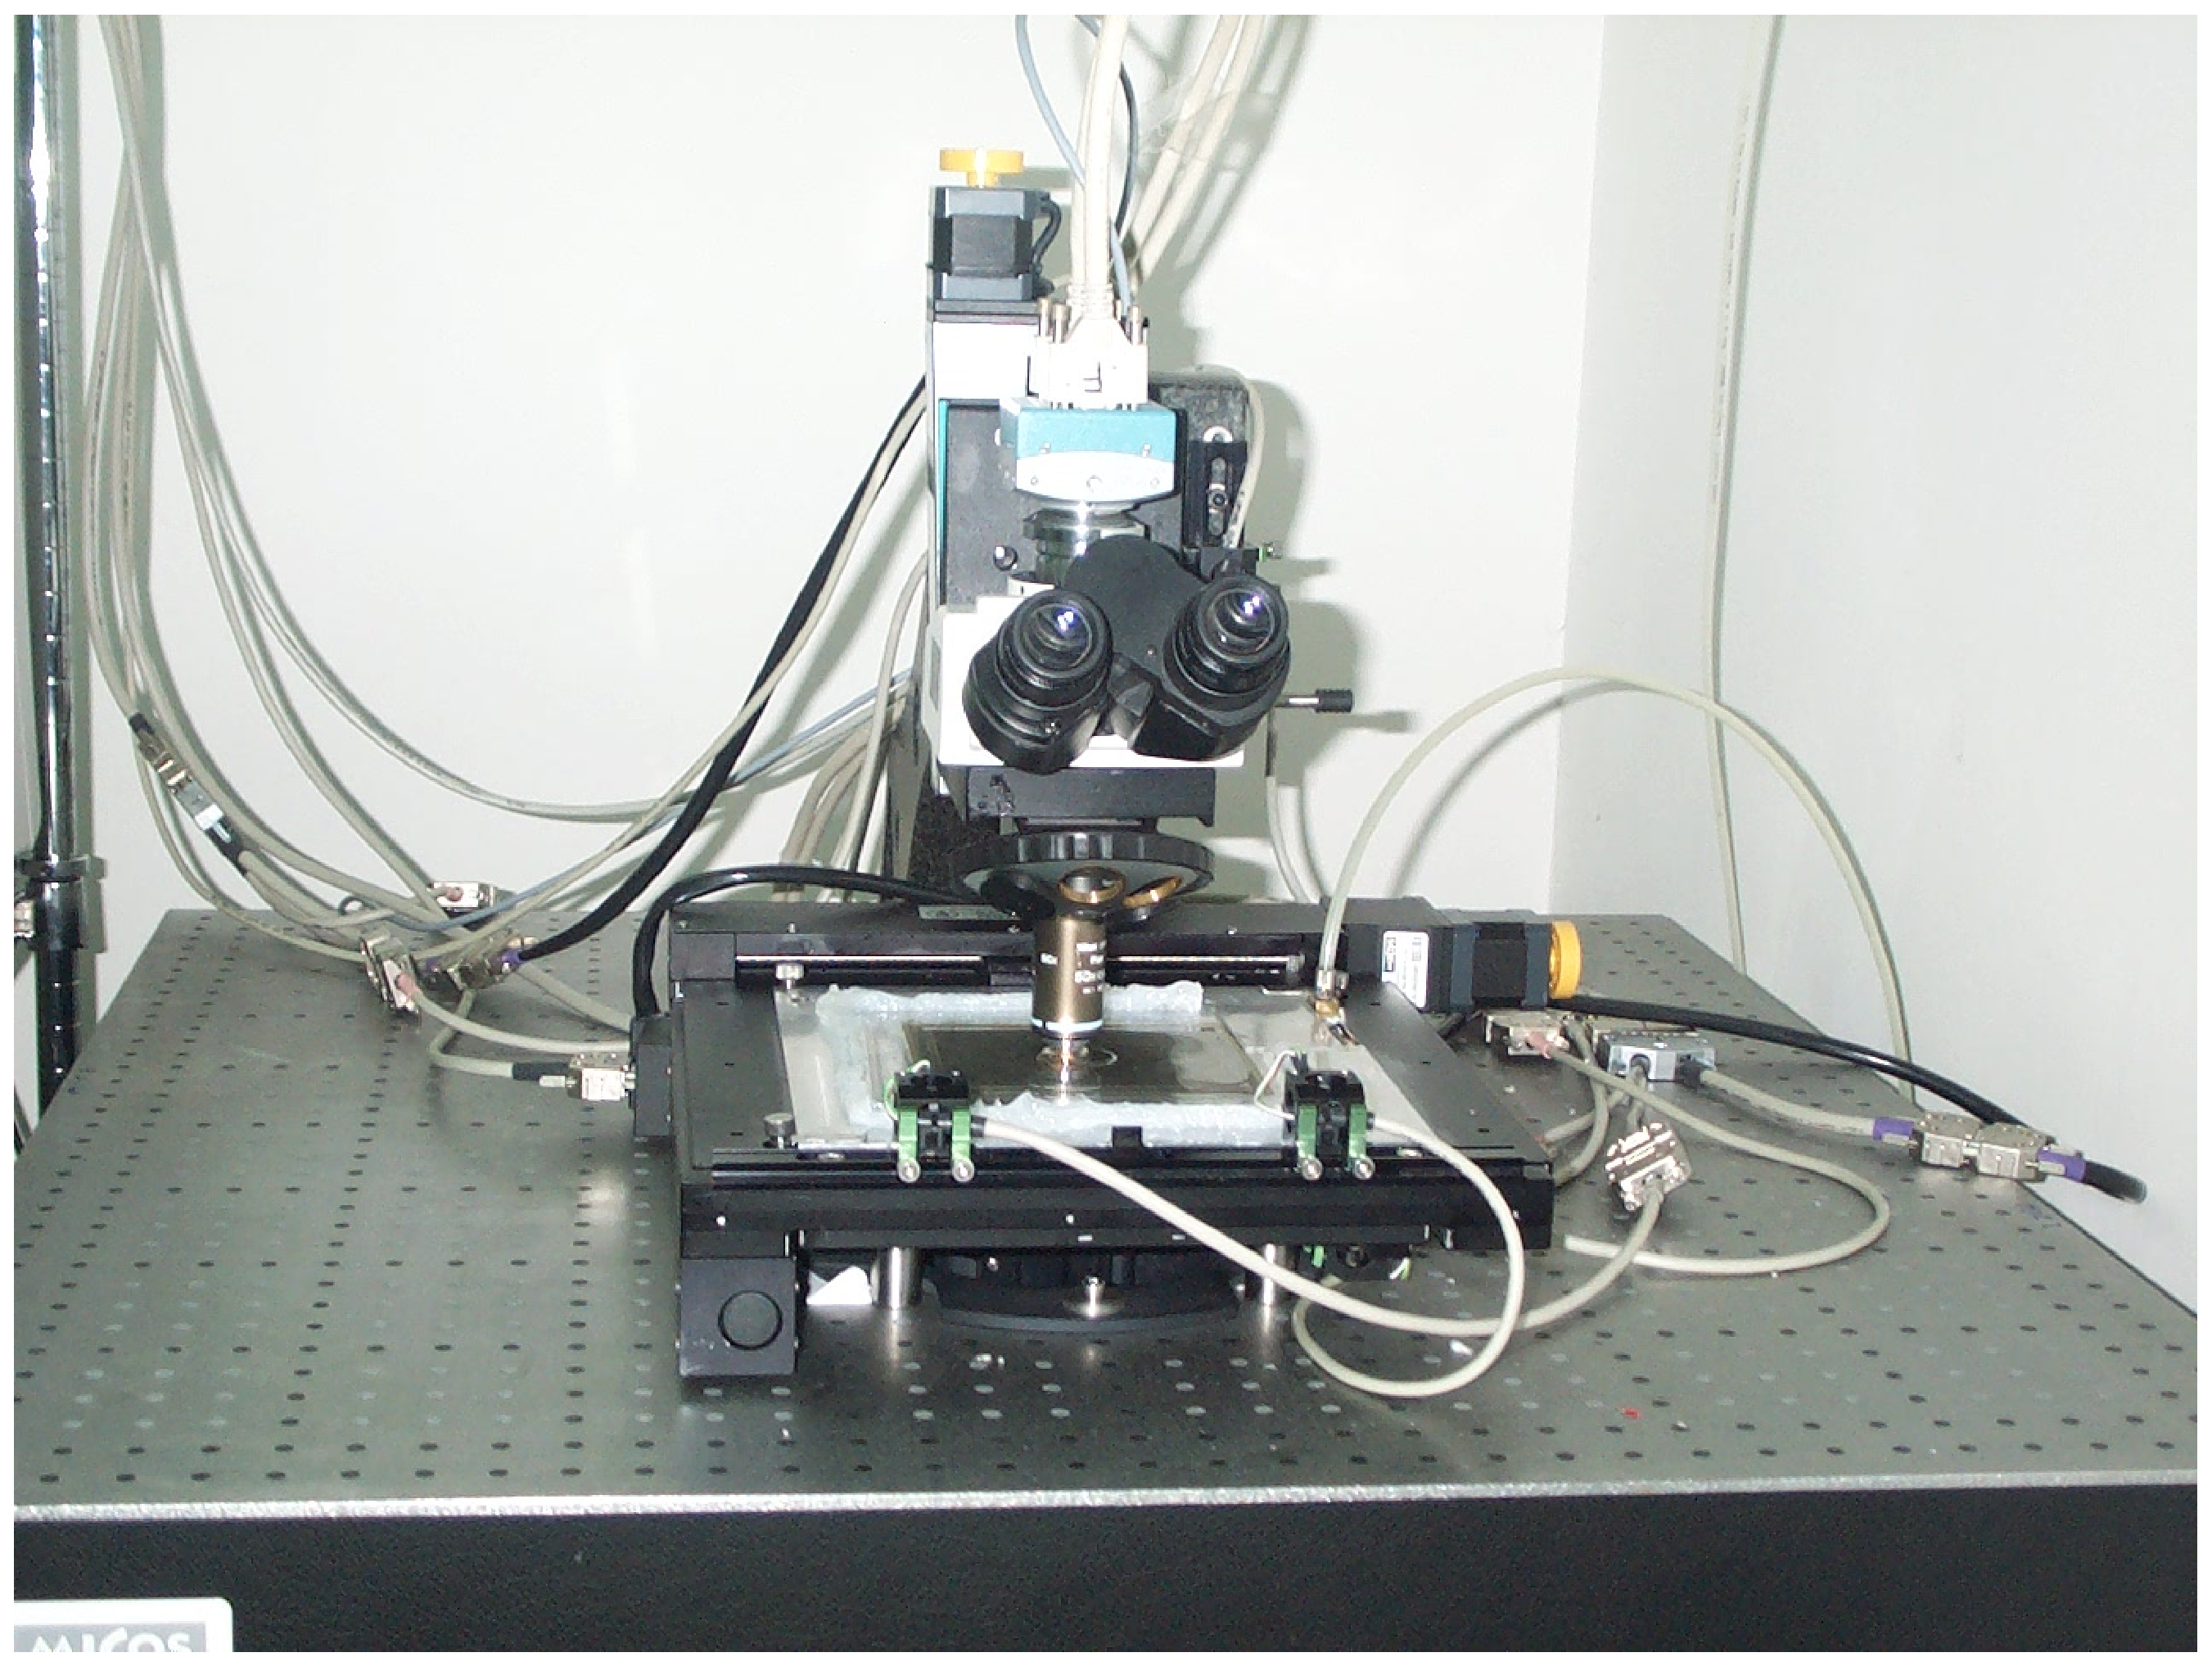
\includegraphics[width=90mm,height=90mm]{./eps/mic2.eps}
\end{center}
\caption{Il sistema ESS}
\label{fig:mic2}
\end{figure}

\begin{figure}[tbp]
\begin{center}
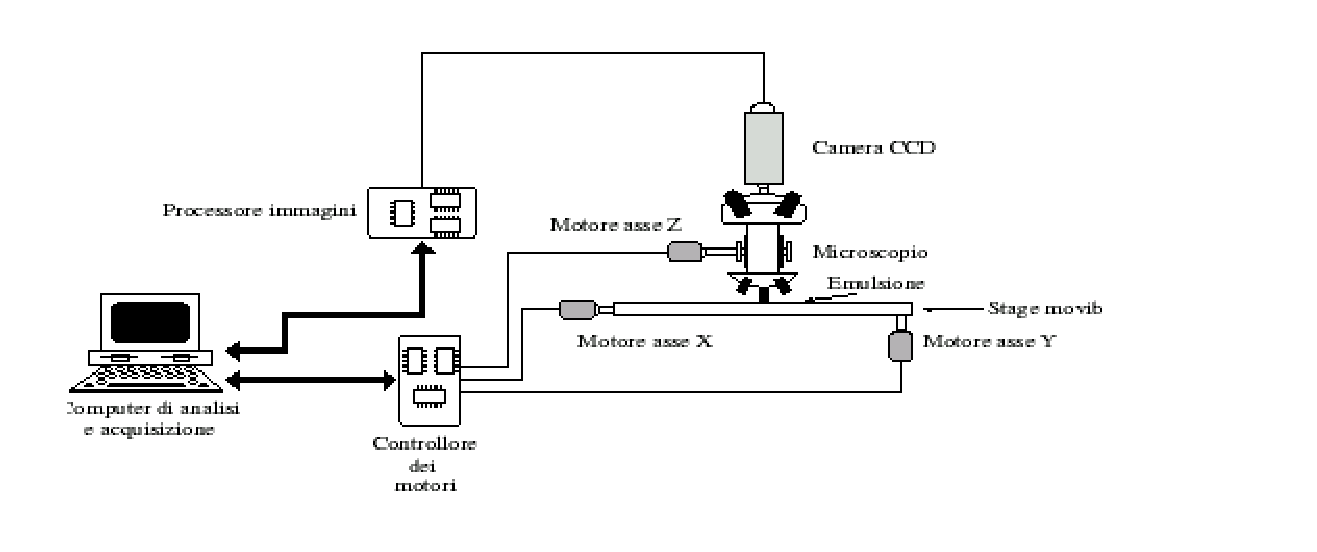
\includegraphics[width=130mm,height=90mm]{./eps/schmic.eps}
\end{center}
\caption{Schema generale del sistema di acquisizione}
\label{fig:mic_schema}
\end{figure}



\subsection{La meccanica di movimentazione e le sue prestazioni}
La meccanica per la movimentazione  � stata realizzata in collaborazione con la  MICOS\footnote{http://www.micos.com/}, un'azienda specializzata nella produzione di meccanica di precisione automatizzata. Nel sistema ESS vengono impiegati:



\begin{itemize}
\item{Un piatto  per il movimento orizzontale $(x,y)$ ;}
\item{Una slitta per la movimentazione verticale del gruppo ottico(asse $z$);}
\item{Un braccio di granito per il supporto della slitta dell'asse $z$ e del gruppo ottico;}
\end{itemize}
Il tutto � montato su di un banco ottico. Il movimento del piatto e del gruppo ottico � controllato da motori passo-passo  a cinque fasi. I motori trasmettono il movimento  mediante una vite micrometrica senza fine  collegata al relativo asse. Questa pu� essere collegata mediante una flangia al piano movibile o direttamente alla slitta. I motori passo passo vengono pilotati tramite impulsi forniti da unit� specifiche di micro-passo e potenza. I motori possono muoversi a 500 passi/giro, corrispondenti a $0.72�/passo$. Le unit� di micro-passo  possono moltiplicare il numero di passi per un fattore fino a 250. L'insieme delle unit� di micropasso, dei motori e delle rispettive viti senza fine consente una velocit� massima di $5cm~/s$ del piatto o della slitta. Allo scopo di mostrare quali sono le prestazioni del sistema motorizzato e per verificare che esse fossero rispondenti alle richieste sono state fatte delle misure del {\em{tempo di assestamento}}. Esso � il tempo necessario affinch� il microscopio  cambi campo di vista attendendo anche   che le oscillazioni del piatto dopo l'arresto, siano contenute entro  $0.2~\mu m$.  In fig. \ref{fig:settx} � riportato l'istogramma dei valori del {\em{tempo di assestamento}} ottenuti con misure ripetute scegliendo opportuni parametri di accelerazione e decelerazione.

\begin{figure}[tbp]
\begin{center}
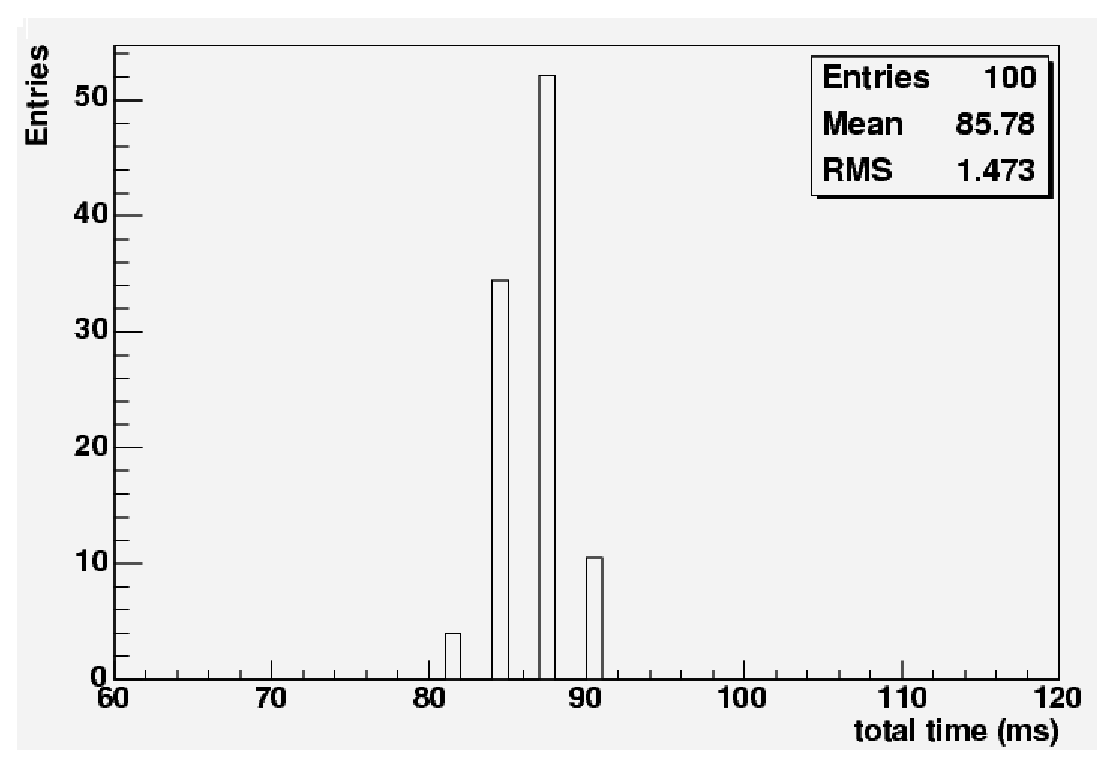
\includegraphics[width=70mm,height=70mm]{./eps/Sett_timeX.eps}
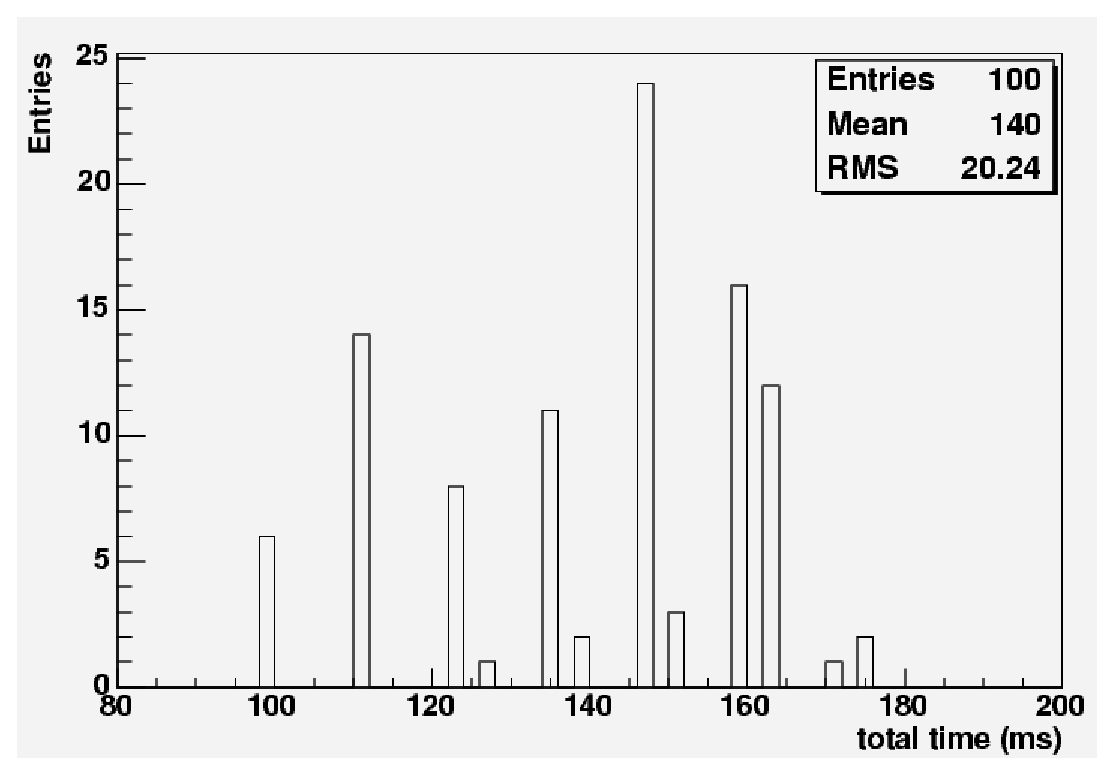
\includegraphics[width=70mm,height=70mm]{./eps/Sett_timeY.eps}
\end{center}
\caption{Misura del tempo di assestamento  per l'asse Y(a destra) e per l'asse Y(a sinistra) incluso il tempo di spostamento da un campo di vista al successivo.}
\label{fig:settx}
\end{figure}

La differenza dei tempi di assestamento dei  due assi �  imputabile  ad una  maggiore inerzia dell'asse $Y$ e quindi un tempo di assestamento maggiore. La differenza di massa � dovuta al fatto che la movimentazione dell'asse $X$  poggia su quella dell'asse $Y$. 
Il software di acquisizione tiene conto di un maggiore tempo di assestamento dell'asse $Y$. Infatti  quando effettua la scansione si muove  principalmente lungo l'asse $X$, limitando gli spostamenti lungo $Y$. La scansione infatti avviene su strisce che si sviluppano lungo l'asse X e gli spostamenti lungo Y sono limitati solo al cambio di striscia.

La posizione del piatto e controllata mediante l'uso di tre encoder lineari di lettura con risoluzione di $0.1 ~\mu m$.
La posizione del piatto viene rilevata dagli encoder istante per istante, durante il movimento. Ci� consente un continuo ricalcolo del numero di passi necessari per il raggiungimento del posizione, migliorando sensibilmente la precisione di posizionamento del sistema. 

\begin{figure}[tbp]
\begin{center}
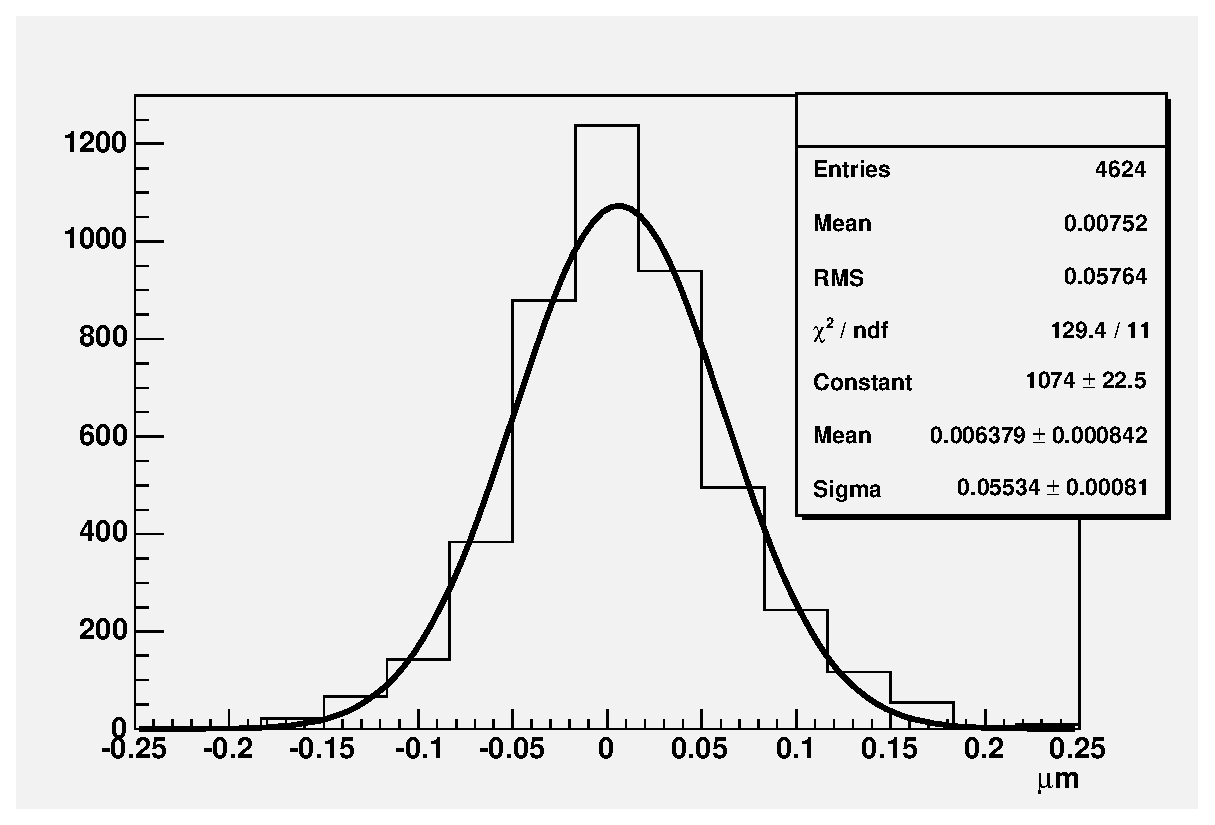
\includegraphics[width=140mm,height=90mm]{eps/Y_clust_pos_10_tracks.eps}
\end{center}
\caption{Misura della precisione di posizionamento per l'asse $Y$. }
\label{fig:precisione}
\end{figure}


La fig. \ref{fig:precisione} rappresenta una misura di precisione di posizionamento dello stage del microscopio. I valori riportati  sono ottenuti realizzando una mappatura completa della superfice disponibile e sono calcolati sottraendola posizione effettivamente raggiunta e misurata dagli "encoder" di posizione al valore di ciascuna coordinata dell zona  analizzata. La movimentazione dell'apparato � controllata da una scheda di controllo motori. Questa scheda � prodotta dalla National Instruments\footnote{http://www.ni.com/} (mod. PCI7344), Essa � dotata di 4 canali per il pilotaggio di motori passo passo e la lettura degli encoders. La scheda � dotata di un Digital Signal Processor(DSP) che ne controlla tutte le funzioni. E' fornita di una libreria, {\bf{FLEX}}, compatibile con i linguaggi C e C++. L'utilizzo del DSP unito alla flessibilit� della libreria permette di programmare e controllare le curve di accellerazione e decellerazione nella fase di posizionamento e di spostamento a velocit� costante, senza l'intervento del computer principale, garantendo la velocit� e precisione richiesta al sistema.

La scheda di controllo motori � anche dotata di 4 DAC a 16 bit associati a canali di pilotaggio motori. Il DAC del quarto canale � utilizzato per il controllo dell'illuminazione del microscopio. Il controllo permette la regolazione dell'intensit� luminosa in modo da ottimizzare le prestazioni dell'ottica e del sistema di acquisizione.

\subsection{La telecamera e il gruppo ottico}
Per consentire l'illuminazione dell'emulsione, sotto il piatto � montata una lampada (fig.\ref{fig:illu}), la cui intensit� � controllabile via software. Un condensatore ottico regolabile in altezza e posizione permette di concentrare la luce all'interno dell'emulsione. Le regolazioni del condensatore permettono di allinearlo all'asse del gruppo ottico e concentrare la luce in modo da garantire  uniformit� di illuminazione. Quest'ultima  � fondamentale per permettere un buon filtraggio dell'immagine. Per evitare che i movimenti del piano possano compromettere l'allineamento del condensatore con l'asse del gruppo ottico e per evitare  che il gruppo ottico danneggi il piano, i binari sono equipaggiati con degli interruttori di fine corsa.

\begin{figure}[tbp]
\begin{center}
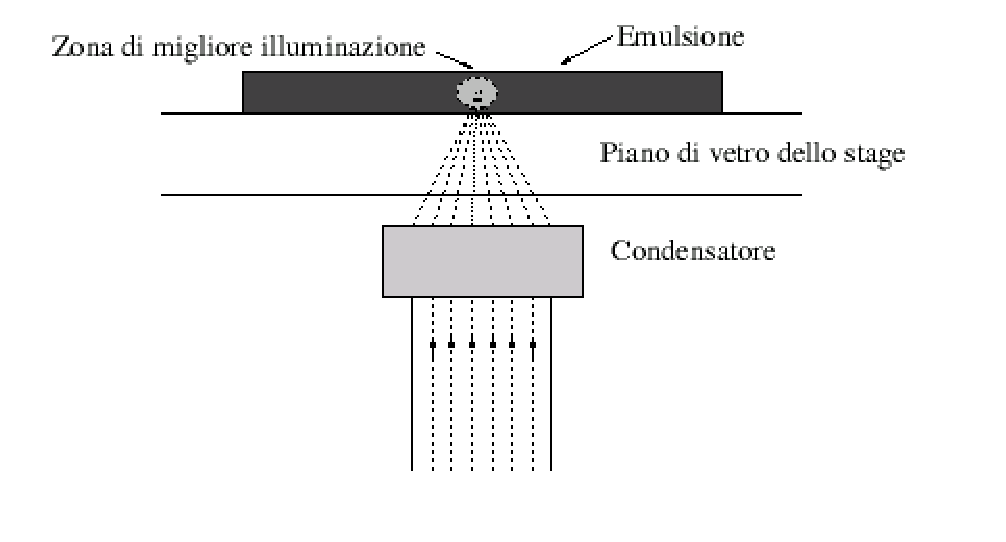
\includegraphics[width=70mm,height=70mm]{./eps/illu.eps}
\end{center}
\caption{Sistema di illuminazione.}
\label{fig:illu}
\end{figure}

   


Il microscopio � dotato di un obiettivo ad olio con una profondit� focale di $0.55\mu m$ e un ingrandimento $50\times$. Le principali aberrazioni  sono corrette all'interno dell'obiettivo. Con la telecamera attualmente in uso si ottiene un campo inquadrato   di $ 394.5\times 315.6 ~\mu m^2$.


La telecamera utilizzata  � il modello MC1310 della Mikrotron. Essa � dotata di un  sensore CMOS, con risoluzione $1280\times1024$ pixel. La dimensione lineare del singolo pixel � di $12\mu m$ la superficie totale inquadrata � di $395.5\times 315.6 \mu m^2$. La telecamera � in grado di acquisire immagini ad una frequenza massima di  500 frames/s, il che implica che un trasferimento dati di $660MB/s$. Il sistema ESS la utilizza ad una frequenza di $376$ frames/s, suffciente a garantire  le prestazioni di scansione richieste.


Le immagini vengono  acquisite e processate mediante l'uso di una scheda MATROX Odyssey. La prima operazione effettuata � quella di eliminare  eventuali piccole impurit� presenti sul sensore della telecamera, utilizzando un'immagine acquisita fuori emulsione e sottraendola alle immagini acquisite in emulsione. La seconda operazione � detta  filtraggio. Questa operazione ha lo scopo di aumentare il contrasto tra i grani messi a fuoco e le ombre dei grani che si trovano al di fuori del frame investigato. Il filtro � ottenuto applicando un matrice di  convoluzione. Il valore del pixel, dopo il filtraggio, � il risultato della somma pesata dei pixel adiacenti secondo l'equazione (\ref{eq:conv}).  
\begin{equation}
p(i,j)=\sum_{h=1}^{6}\sum_{k=1}^{6}K(h,k)\cdot g(i+h,j+k)
\label{eq:conv}
\end{equation}

Gli studi effettuati hanno portato a utlizzare come  filtro  la seguente matrice $6\times 6$ \cite{ESSA}:

\begin{equation}
\nonumber K \; = \;\;
\begin{array}{|c|c|c|c|c|c|}
  \hline
  1 &  1 &  1  &  1  & 1 & 1 \\ \hline
  1 & 2 &  3  &  3  & 2 & 1 \\ \hline
  \;1\; & \;3\; & -13 & -13 &\; 3 \;&\; 1 \; \\ \hline
  1 & 3 & -13 & -13 & 3 & 1 \\ \hline
  1 & 2 &  3  &  3  & 2 & 1 \\ \hline
  1 & 1 &  1  &  1  & 1 & 1 \\ \hline
\end{array}
\end{equation}





Dopo il filtraggio viene applicata una soglia  e l'immagine vine binarizzata: ai pixel con valore che superano la soglia viene assegnato il valore 1, 0 agli altri. L'ultima operazione effettuata dal processore del computer � l'individuazione dei cluster e della loro area. Le informazioni dei cluster sono utilizzate dal software di ricostruzione delle tracce.

Per verificare il corretto allineamento dell'asse $Z$  si possono confrontare le distribuzioni angolari acquisite in due differenti scansioni: usando nella  prima una   regione di emulsione  e, nella seconda, la stessa regione ruotando il foglio di 180 gradi. Il disallinemamento viene misurato confrontando la differenza delle distribuzioni angolari  delle due scansioni per un determinato angolo.In fig.\ref{fig:zslant}  sono riportate le  distribuzioni angolari delle due scansioni, dalle quali si evince che la differenza angolare tra i due valori centrali \'{e} di circa $2~mrad$.


\begin{figure}[tbp]
\begin{center}
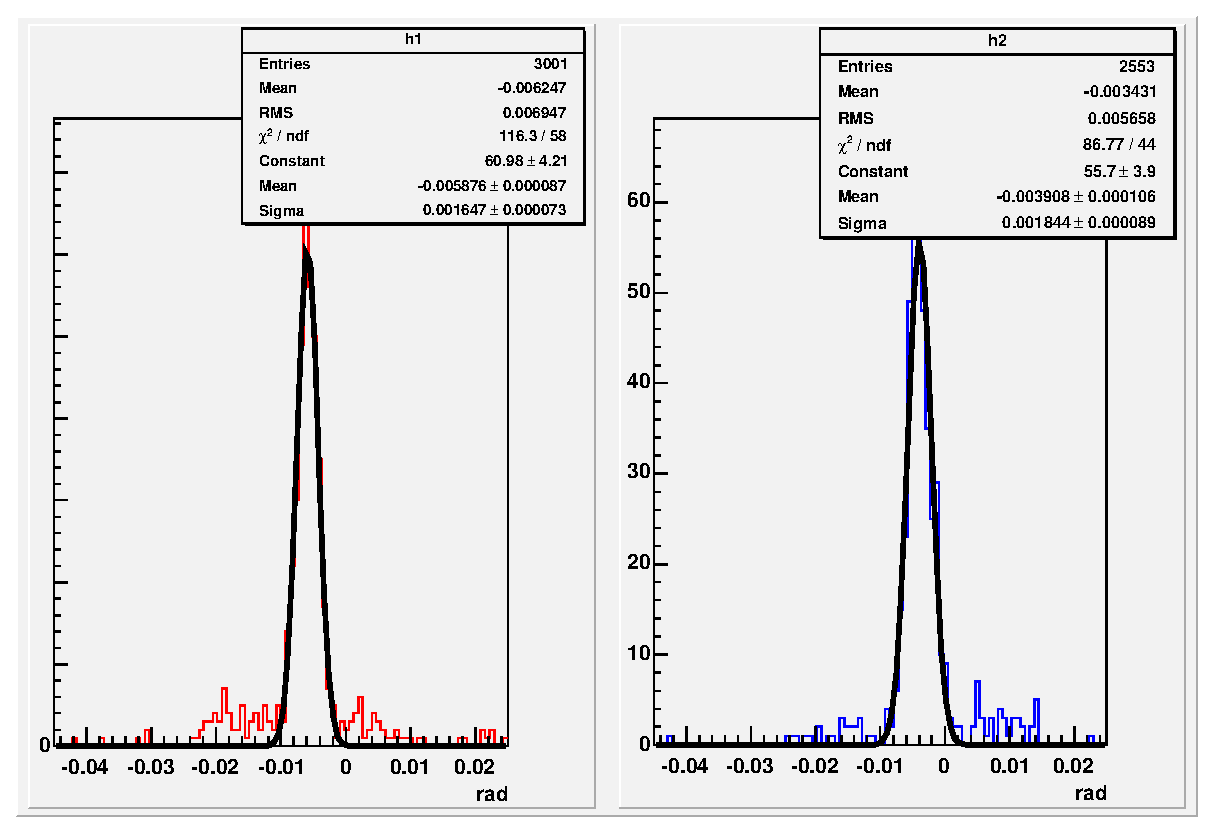
\includegraphics[width=120mm,height=80mm]{eps/Zslant.eps}
\end{center}
\caption{Allineamento della telecamera e dell'asse Z}
\label{fig:zslant}
\end{figure}

\subsection{Software di acquisizione}
Il software di acquisizione on-line per la scansione automatica delle emulsioni e la ricostruzione dei segmenti delle tracce � stato sviluppato in ambiente C++. Esso � basato su una struttura modulare dove  ogni oggetto svolge un ben  definito compito. Per ogni oggetto � possibile controllare e variare i parametri. 
Il  software gestisce sia la  movimentazione dei tre assi, che il processamento e la ricostruzione dei segmenti nell'area di emulsione analizzata. I dati relativi alla scansione vengono  salvati in files binari.

E' importante misurare le quote di ingresso e uscita degli strati di emulsioni e della parte insensibile (base) del film. Il microscopio si muove lungo l'asse $Z$ e  misura il numero di cluster per campo a differenti  quote. La fine di uno strato di emulsione � definita quando il numero di clusters � minore di una determinata soglia. Dopo questa operazione vengono acquisiti i frame ai vari livelli  e ricostruiti i  segmenti, le cosidette microtracce, nei due strati di emulsione da una parte e l'atra della base.
La ricostruzione delle microtraccie � divisa in due fasi: riconoscimento dei  grani appartenenti alla micro traccia  e successivo fit lineare.

La ricerca di una microtraccia avviene cercando seguenze di grani allineati apparteneti a diversi strati dell'emulsione. Per ridurre il numero di possibili combinazioni di grani, il campo � diviso in celle, la cui dimensione lineare � circa $25~ \mu m$. Il primo passo nella determinazione della microtraccia � la ricerca del trigger. I livelli  di ogni buccia di emulsione sono numerati da 1 a 16. Sono definite delle sequenze di trigger. Una sequenza � formata da un livello appartente al settore superiore della strato, un livello  appartenente al settore inferiore  e qualche livello appartenente al settore centrale. Per ogni dato trigger vengono effettuate tutte le combinazioni di grani tra il livello superiore  e quello inferiore, definito nella sequenza. Per ogni combinazione vengono cercati i cluster nei livello  centrali, della sequenza di trigger entro una definita accettanza. Se almeno un grano � trovato in uno dei layer centrali, viene generato un segnale di trigger. Il numero di sequenze di trigger e il numero di livelli richiesti in tali sequenze � stato ottimizzato tramite simulazioni Monte-Carlo. 

Una volta ottenuto un segnale di triggervengono cercati  i grani in tutti gli altri livelli. Mentre per la definizione del trigger  vengono usati esclusivamente grani appartenenti alla stessa cella, in questo caso anche le celle adiacenti sono prese in considerazione.  Se il numero di grani trovati supera una determinata soglia viene definita una microtraccia. Un fit lineare dei grani viene effettuato per determinare gli angoli e la posizione della microtraccia. Tale informazione viene salvata nei files di uscita.


\section{Ricostruzione delle tracce di base}
Il sistema di acquisizione online ricostruisce le microtracce all'interno dei due strati di emulsioni dell' ES. 
A partire dalle microtracce vengono ricostruite le tracce di base attraverso la connessione dei grani pi� vicini  alla base  nelle microtracce dei due fogli i emulsioni. 

Per la ricostruzione delle traccie di base, le microtracce vengono proiettate  al centro della  base e vengono cercate le coppie in base all'accordo angolare ed in posizione.

\begin{figure}[tbp]
\begin{center}
\includegraphics[width=90mm,height=90mm]{eps/updown.eps}
\end{center}
\caption{Il principio della ricostruzione delle tracce di base.}
\label{fig:tch}
\end{figure}

La traccie di base sono selezionate in base al valore del $\chi^2$ definito mediante la sequente equazione:

\begin{equation}
\chi^2 = \frac{1}{4} \left[ \frac{(\theta_{Xt} - \theta_{XB})^2}{\sigma^2_X} + \frac{(\theta_{Xb} - \theta_{XB})^2 }{\sigma^2_X} +\frac{(\theta_{Yt} - \theta_{YB})^2 }{\sigma^2_Y} + \frac{(\theta_{Yb}- \theta_{YB})^2 }{\sigma^2_Y} \right]
\label{eq:linkud}
\end{equation}

dove $\theta_{X(Y)b(t)}$ sono  le proiezioni angolari X(Y) delle   
microtraccie dello strato  superiore, $\theta_{X(Y)B}$ dello strato  inferiore 
 e $\sigma_{X,Y}$ indica  la risoluzione angolare della  microtraccia. \\


In fig. \ref{fig:tchi2} � mostrata la distribuzione $\chi^2$ nei dati. Si vede chiaramente il segnale per valori di $\chi^2<3$, mentre il fondo domina per valori pi� alti. 


\begin{figure}[tbp]
\begin{center}
\includegraphics[width=80mm,height=80mm]{eps/chi2.eps}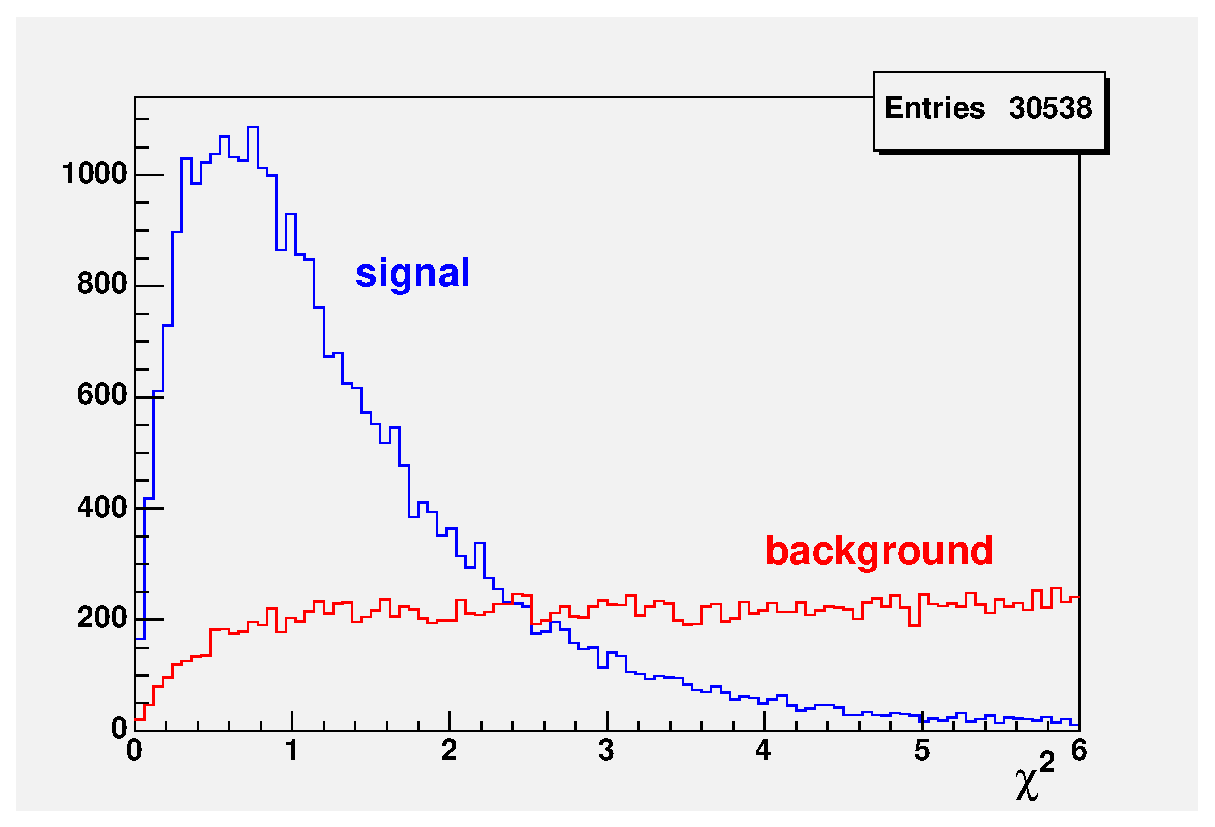
\includegraphics[width=80mm,height=80mm]{eps/tchi2.eps}

\end{center}
\caption{Distribuzione di $\chi^2$ nei dati (sinistra). Nel grafico a destra sono state selezionate tracce di solo segnale e solo fondo per evidenziarne i due caratteri. Il grafico a sinistra \'{e} la loro somma. }
\label{fig:tchi2}
\end{figure}

La risoluzione angolare di microtraccia � definita in base all'accordo tra l'angolo della microtraccia e quello della traccia di base da essa formata. Questo parametro indica  l'accuratezza  angolare del microscopio e l'eventuale presenza di vibrazioni meccaniche. In fig. \ref{fig:res}
viene mostrata la risoluzione angolare di microtraccia  per $\theta_x=0$ sia nella proezione X che Y. La risoluzione angolare degrada al variare dell'angolo, come atteso. Tale degradazione viene  parametrizzata con buona approssimazione come $\sigma(\theta)=\sigma(0)(1+4\cdot |\theta|)$.
La dipendenza della risoluzione di microtraccia  dall'angolo � dovuta all'incertezza sulla posizione Z dei grani.  Considerando un sistema di riferimento bidimensionale XZ, e per un fissato spessore delle emulsioni $\delta Z$, se assumiamo che la coordinata Z sia  priva di errore (considerandola la variabile indipendente nella procedura di fit), l'errore indotto sulla posizione X � proporzionale alla tangente dell'angolo della microtraccia.

\begin{figure}
\begin{center}
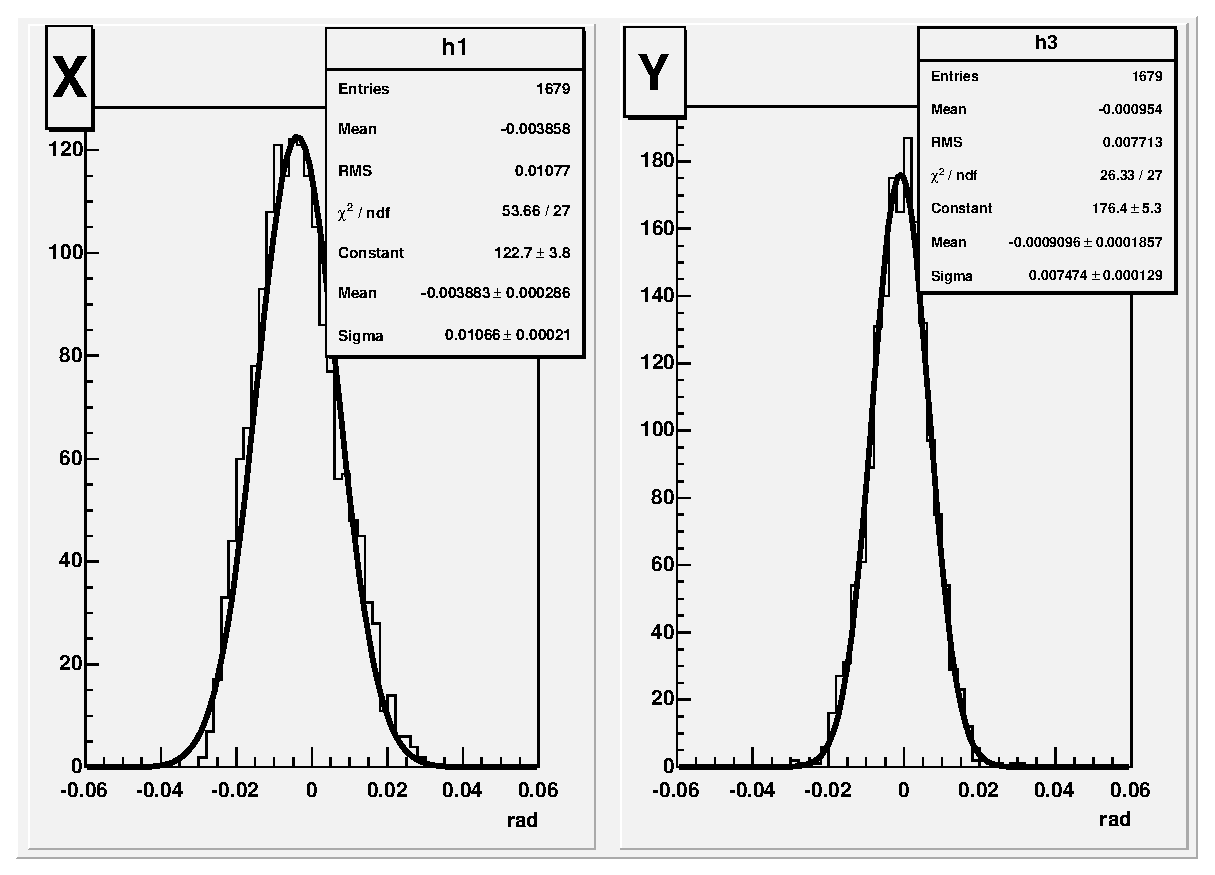
\includegraphics[width=120mm,height=90mm]{eps/res.eps}
\end{center}
\caption{Risoluzione angolare nella ricostruzione di microtracce. }
\label{fig:res}
\end{figure}

Il numero di grani per traccia dipende dalla sensibilit� delle emulsione. Per l'esperimento OPERA la sensibilit� delle emulsioni e' di $33~grani/100~\mu m$. Una traccia verticale che attraversa uno strato di emulsione ha in media $42\times(33/100)=13.9$ grani. Considerando i due strati, le tracce di base devono avere in media 27.8 grani, il che � in buon accordo con il valore misurato  riportato in figura \ref{fig:pulse}.

\begin{figure}[tbp]
\begin{center}
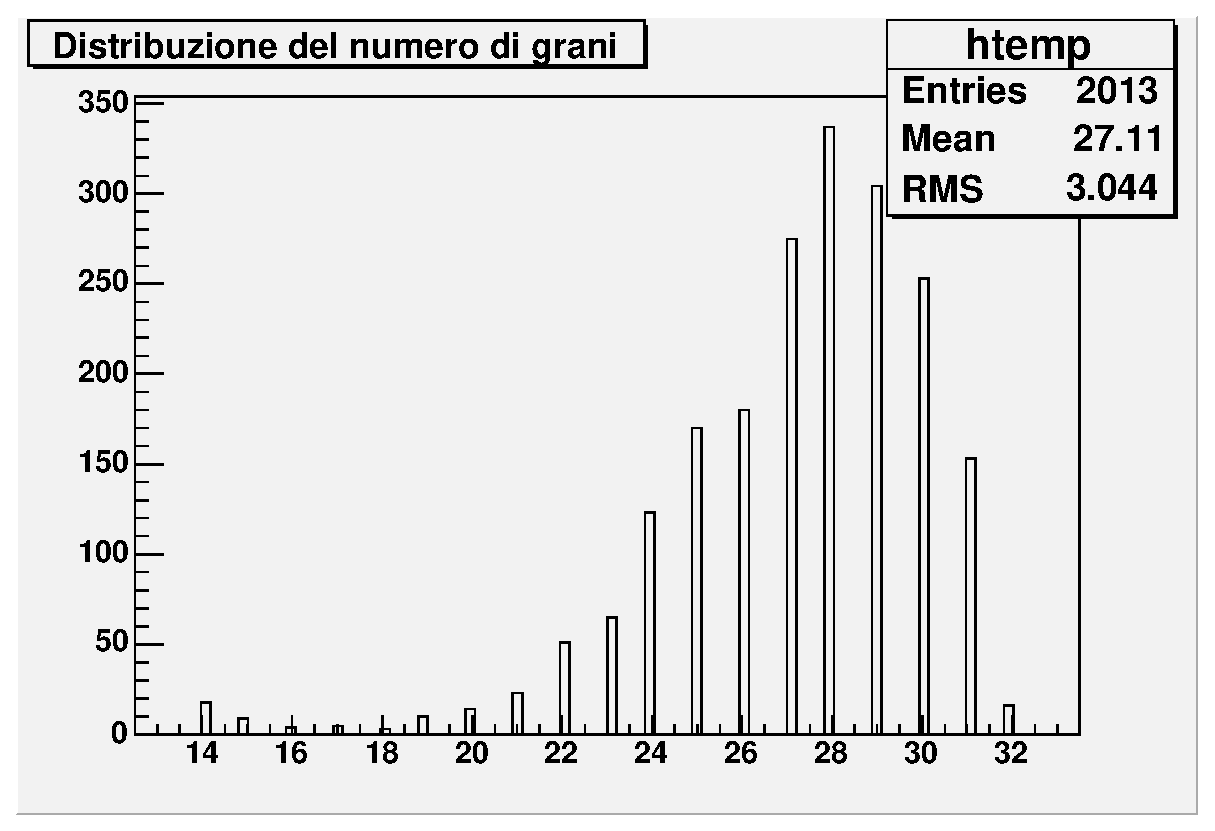
\includegraphics[width=90mm,height=90mm]{eps/pulse_eff.eps}
\end{center}
\caption{Distribuzione del numero di livelli pieni su un totale di 32 livelli acquisiti sui due strati. }
\label{fig:pulse}
\end{figure}

\section{Ricostruzione delle tracce nelle ECC}

Come mostrato in fig. \ref{fig:track} le tracce di base sono utilizzate per la ricostruzione di tracce che hanno attraversato varie celle ECC. Durante l'impacchettamento delle lastre di emulsione e piombo, i film sono in generale roto-traslati tra loro. Per poter ricostruire le traccie che attraversano diverse celle � necessario,  correggere le rototraslazioni riscontrate. Ci\'{o} viene fatto mediante algoritmi di riconoscimento di pattern su coppie di lastre consecutive, con una procedura che prende il nome di {\emph{intercalibrazione}}.

\begin{figure}[tbp]
\begin{center}
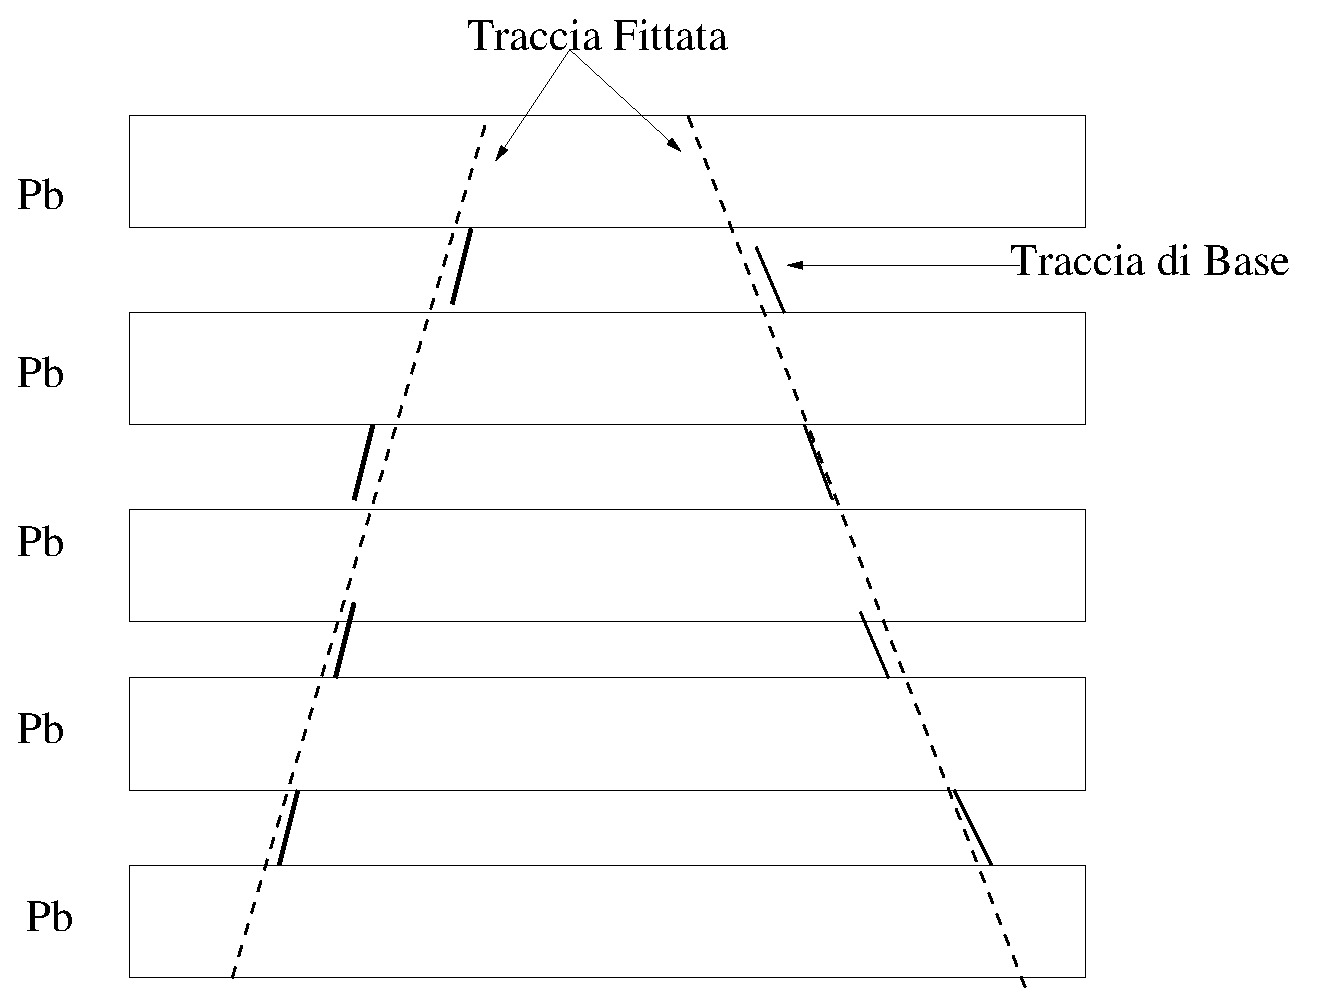
\includegraphics[width=90mm,height=90mm]{eps/track.eps}
\end{center}
\caption{Disegno schematico di una ECC costituita da 5 celle.Sono mostrate due tracce (tratteggiate) e le corrispondenti tracce di base(continue). }
\label{fig:track}
\end{figure}


L'intercalibrazione di due lastre consecutive  viene effettuata applicando diverse traslazioni alle tracce di base in posizione e calcolando il numero di tracce associate ad ogni spostamento. La corretta traslazione dei piatti � individuata dalla massimizzazione del  numero di associazioni. Dopo aver ricavato l'entit� della traslazione, viene calcolata la trasformazione affine tra i due fogli la quale tiene conto anche delle  rotazioni e deformazione tra i fogli di emulsione. La trasformazioni affine � definita nel seguente modo:


\begin{equation}
\left( \begin{array}{c} x' \\ y' \\ \end{array} \right) = \left(
\begin{array}{cc} a_{11} & a_{12} \\ a_{21} & a_{22} \\\end{array}
\right) 
\left( \begin{array}{c} x \\ y  \\\end{array} \right) + \left(\begin{array}{c} b_{1} \\ b_{2}  \\\end{array}
\right) 
\end{equation}

Utilizzando circa un centinaio  di traccie passanti si riesce ad ottenere un allineamento dell'ordine del micron.


Una volta che i piatti sono stati allineati � possibile passare alla ricostruzione delle tracce. L'algoritmo per la ricostruzione delle traccie si basa essenzialmente sullo stesso metodo utilizzato per la ricostruzione delle tracce di base. Partendo da coppie di tracce di base, si tenta di estenderle da entrambi i lati combinandole con altre tracce di base. La catena di tracce di base \'e interrotta in presenza di un decadimento o interazione oppure per inefficienze nelle determinazione delle tracce di base. Una procedura, detta di {\emph{relink}}, success ivamente prova ad unire  i  pezzi della stessa  traccia non connessi. La catene di tracce di base vengono fittate utilizzando  Kalman fit \cite{Kalman}. La risoluzione in posizione  delle tracce di base � ottenuta dai residui in posizione  delle tracce di base rispetto alle tracce fittate su diversi fogli di emulsione (fig. \ref{fig:resbase}).

\begin{figure}[tbp]
\begin{center}
\includegraphics[width=90mm,height=90mm]{eps/btrk_pos_res.eps}
\end{center}
\caption{Risoluzione della traccia di base. }
\label{fig:resbase}
\end{figure}




\section{ Efficienza di tracciamento.}

Per la misura di efficienza sono stati utilizzati fogli di emulsione nucleari di un brick  esposto ad un fascio di pioni dell'energia di $8~GeV/c$ con  vari angoli di incidenza, in modo da avere una misura dell'efficienza al variare dell'angolo del fascio fig. \ref{fig:eff_angle}. Per  evitare effetti spuri dovuti a  deviazioni dell'angolo delle tracce tra i vari fogli dovuto alla diffusione Columbiana, il brick � stato assemblato utilizzando solo fogli di emulsioni, nonintervallate da lastre di piombo come di rigola avviene in OPERA.

\begin{figure}[tbp]
\begin{center}
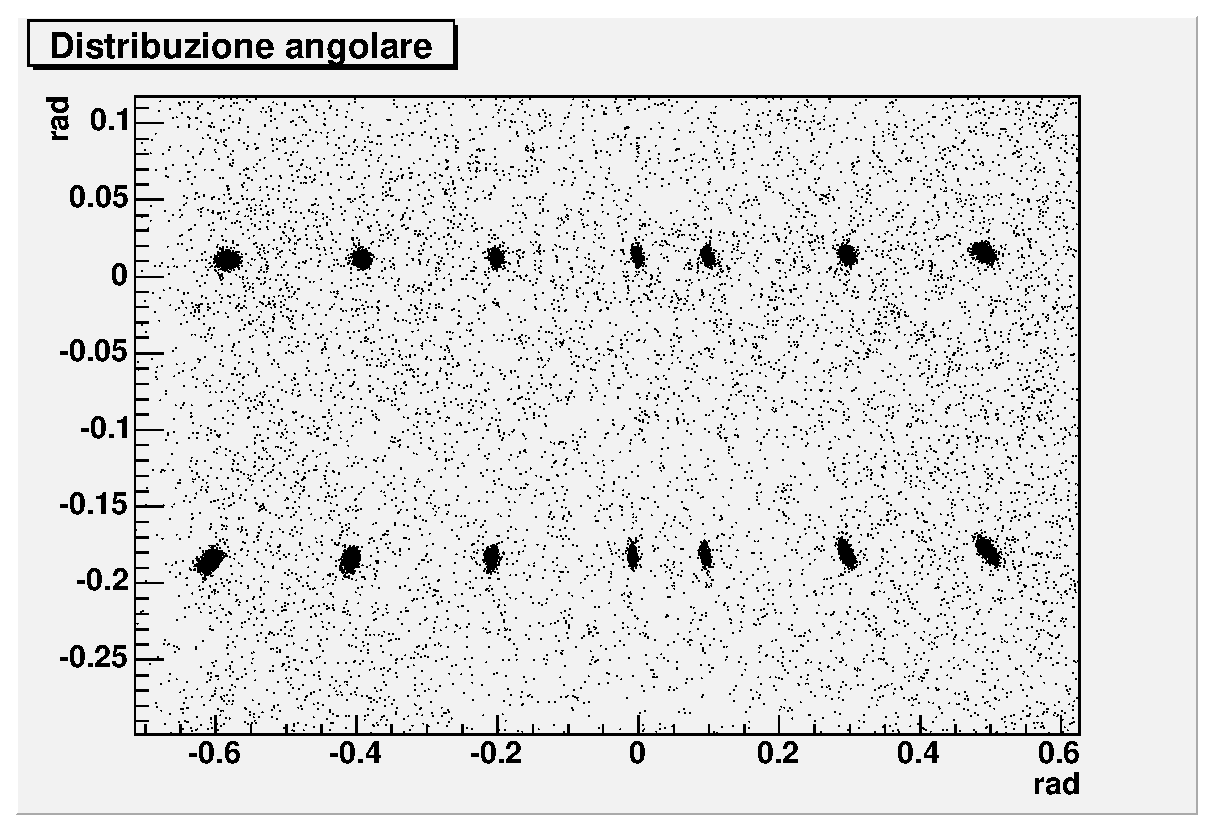
\includegraphics[width=120mm,height=80mm]{eps/eff_angle.eps}
\end{center}
\caption{Distribuzione angolare delle tracce }
\label{fig:eff_angle}
\end{figure}



Si � effettuata una  scansione circa $4~cm^2$ su 8 piatti consecutivi. I dati acquisiti sono stati processati seguendo i passi descritti in precedenza: ricostruzione delle tracce di base, intercalibrazione dei piatti, ricostruzione delle tracce.


Per il calcolo dell'efficienza si considerano tutte le tracce trovate su un certo numero di fogli di emulsione. Nel   foglio immediatamente successivo si verifica se  la traccia di base associata � presente o meno(si veda figura \ref{fig:eff}). Usando tracce trovate su 4 fogli consecutivi come campione di normalizzazione, l'efficienza � definita da

\begin{equation}
\epsilon=\frac{N5}{N4+N5}
\end{equation}

dove $N4$ e $N5$ sono il numero di tracce avente rispettivamente 4 e 5 segmenti consecutivi. Avendo effettuato la scansione di 8 fogli consecutivi � possibile realizzare 8 misure indipendenti dell'efficienza. 
La scelta di utilizzare quintupletti su quadrupletti deriva da due fattori: in primo luogo si \'{e} osservato che gi\'{a} con i quadrupletti il livello di coincidenze casuali \'{e} trascurabile e pertanto il risultato non cambia se si utilizzano tracce a pi\'{u} segmenti. In secondo luogo, avendo a disposizione 8 lastre, l'utilizzo di quadrupletti consente di mediare su 8 combinazioni, migliorando l'accuratezza statistica della misura.
La media sulle 8 misure � riportata in tabella \ref{tab:eff}, con il suo relativo errore, per i vari angoli di incidenza del fascio.
\begin{figure}[tbp]
\begin{center}
\includegraphics[width=90mm,height=90mm]{eps/eff.eps}
\end{center}
\caption{Definizione delle tracce utilizzate per la misura di efficienza.}
\label{fig:eff}
\end{figure}


\begin{table}[h!]
\begin{center}
\begin{tabular}{|c|c|c|}
  \hline
  % after \\: \hline or \cline{col1-col2} \cline{col3-col4} ...
  $\theta_x$ (rad) & $\theta_y$ (rad) & $\varepsilon$ ($\%$) \\
  \hline
  $0.010$ & $0.015$ & $93.7 \pm 1.4$ \\
  $0.093$ & $0.014$ & $92.5 \pm 1.3$ \\
  $0.211$ & $0.017$ & $89.5 \pm 1.7$ \\
  $0.294$ & $0.012$ & $86.4 \pm 2.3$ \\
  $0.405$ & $0.019$ & $85.2 \pm 2.3$ \\
  $0.492$ & $0.011$ & $87.2 \pm 2.0$ \\
  $0.017$ & $0.184$ & $88.1 \pm 2.0$ \\
  $0.088$ & $0.184$ & $87.3 \pm 2.7$ \\
  $0.220$ & $0.183$ & $85.7 \pm 1.4$ \\
  $0.291$ & $0.185$ & $86.4 \pm 2.3$ \\
  $0.423$ & $0.181$ & $87.2 \pm 1.6$ \\
  $0.495$ & $0.187$ & $88.7 \pm 2.0$ \\
 \hline
\end{tabular}
\caption{Misura di efficienza di tracciamento con lastre esposte al fasci di pioni di $8GeV$ al CERN.}
\label{tab:eff}
\end{center}
\end{table}

\begin{figure}[tbp]
\begin{center}
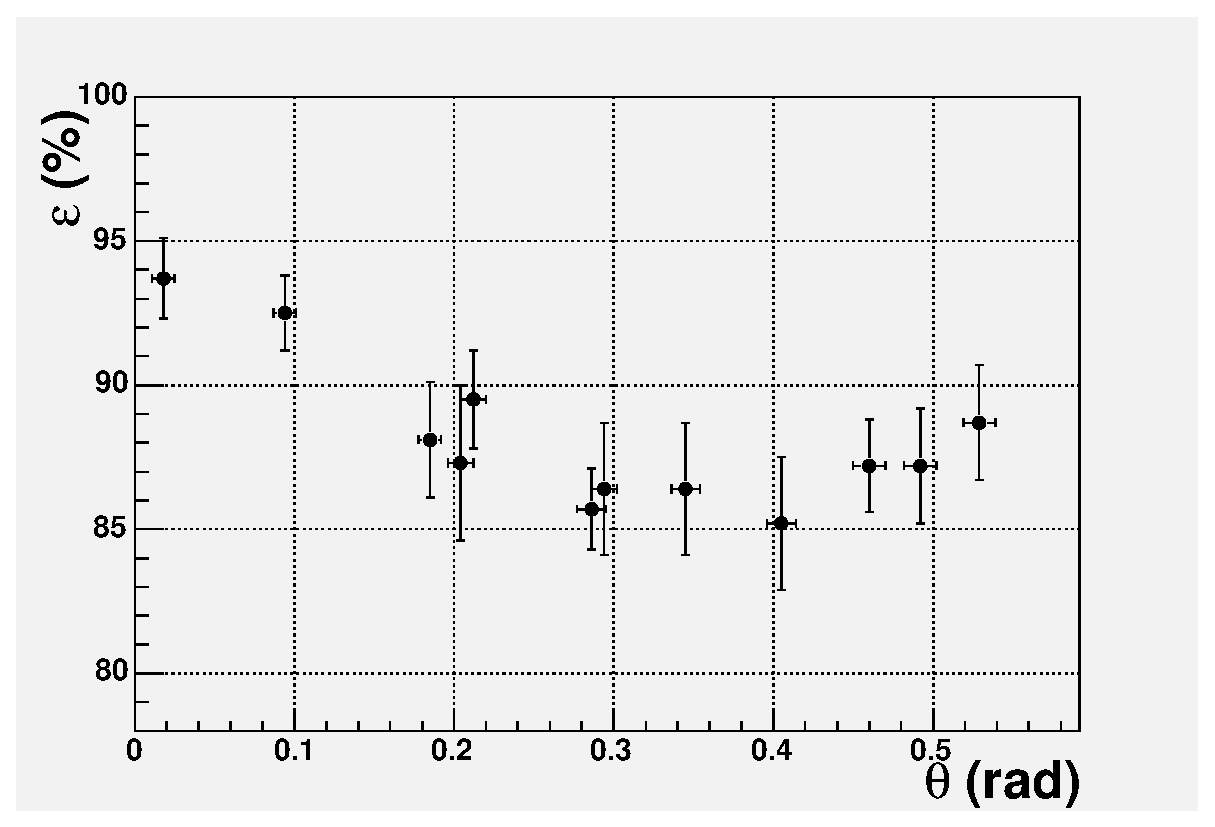
\includegraphics[width=90mm,height=90mm]{eps/efficiency.eps}
\end{center}
\caption{Misura dell'efficienza in funzione dell'angolo della traccia.}
\label{fig:effangle}
\end{figure}



\chapter{Localizzazione dei vertici}

Considerate la caratteristiche del fascio CNGS (sec. \ref{sec:cngs}),
il numero atteso di interazioni di neutrino � di circa 50 al
giorno. Il muro e il mattone in cui � avvenuta una interazione sono
individuati grazie alle informazioni dei rivelatori elettronici. Il
mattone viene quindi rimosso e da esso viene staccato il porta-CS con
i CS ad esso collegati.  Il numero di CS non � ancora definito del
tutto: si potranno avere uno o due CS. Le prove su fascio sono state
comunque fatte con due CS, soprattutto tenendo conto dell'alta densit�
di tracce spurie nei fogli di emulsione per esse utilizzati.  Nel
testo successivo ci si riferir� pertanto a due CS.

I CS vengono sviluppati e su di essi viene effettuata una scansione
per la ricerca delle tracce prodotte nell'interazione di neutrino. Nel
caso di una interazione di corrente carica, viene analizzata una
regione di $5\times5 ~cm^2$ attorno alla zona predetta. Nel caso di
interazione di corrente neutra viene analizzata tutta l'area dei
CS. Se vengono ricostruite una o pi� traccie nei CS, si procede alla
rimozione del mattone corrispondente. L'analisi dei CS serve a meglio
localizzare l'interazione e a confermare se il mattone estratto �
quello corretto o se si deve procedere all'estrazione di un altro
mattone.

Prima di essere disassemblato per lo sviluppo delle emulsioni, il
 mattone estratto viene esposto a raggi cosmici in modo da accumulare
 un numero di tracce passanti adeguato per effettuare
 l'intercalibrazione tra i piatti. L'analisi del mattone viene
 effettuata mediante la procedura di Scan Back. Questa procedura
 consiste nell'inseguire a ritroso rispetto al fascio le tracce
 trovate nei CS, partendo dal foglio di emulsioni pi� a valle nel
 mattone.  Le tracce vengono ricercate in un intervallo angolare
 determinato in base all'accuratezza della predizione e tenendo conto
 della possibile distorsione delle emulsioni. In questo lavoro di tesi
 � stata studiata questa procedura e verificata la sua validit�,
 mediante prove su fascio.



\section{La presa dati su fascio}

Per studiare come ricostruire vertici di interazioni mediante la
 procedura di Scan Back � stato realizzato un mattone con 56 celle di
 emulsioni e piombo, corredato da due CS situati a valle rispetto al
 fascio.

I fogli di emulsione utilizzati per queste prove su fascio sono state
trasportati in aereo dal Giappone fino in Italia, quindi hanno
accumulato una elevato flusso di cosmici. Per ridurre il numero di
tracce, prima dell'assemblaggio del mattone al CERN � stato effettuato
un processo di {\emph{refreshing }}. Il refreshing consiste nel
mantenere per alcuni giorni le emulsioni a una temperatura di $30�$ e
umidit� relativa del $\sim 95\%$.  Questa procedura consente di
ridurre le immagini latenti accumulate.


Il mattone � stato esposto a un fascio di pioni con energia di 8 $GeV$
e con un'angolo di incidenza di $50~mrad$ nella proiezione $X$. Le
prove sono state effettuate utilizzando il fascio di pioni del CERN
PS.
\begin{figure}[tbp]
\begin{center}
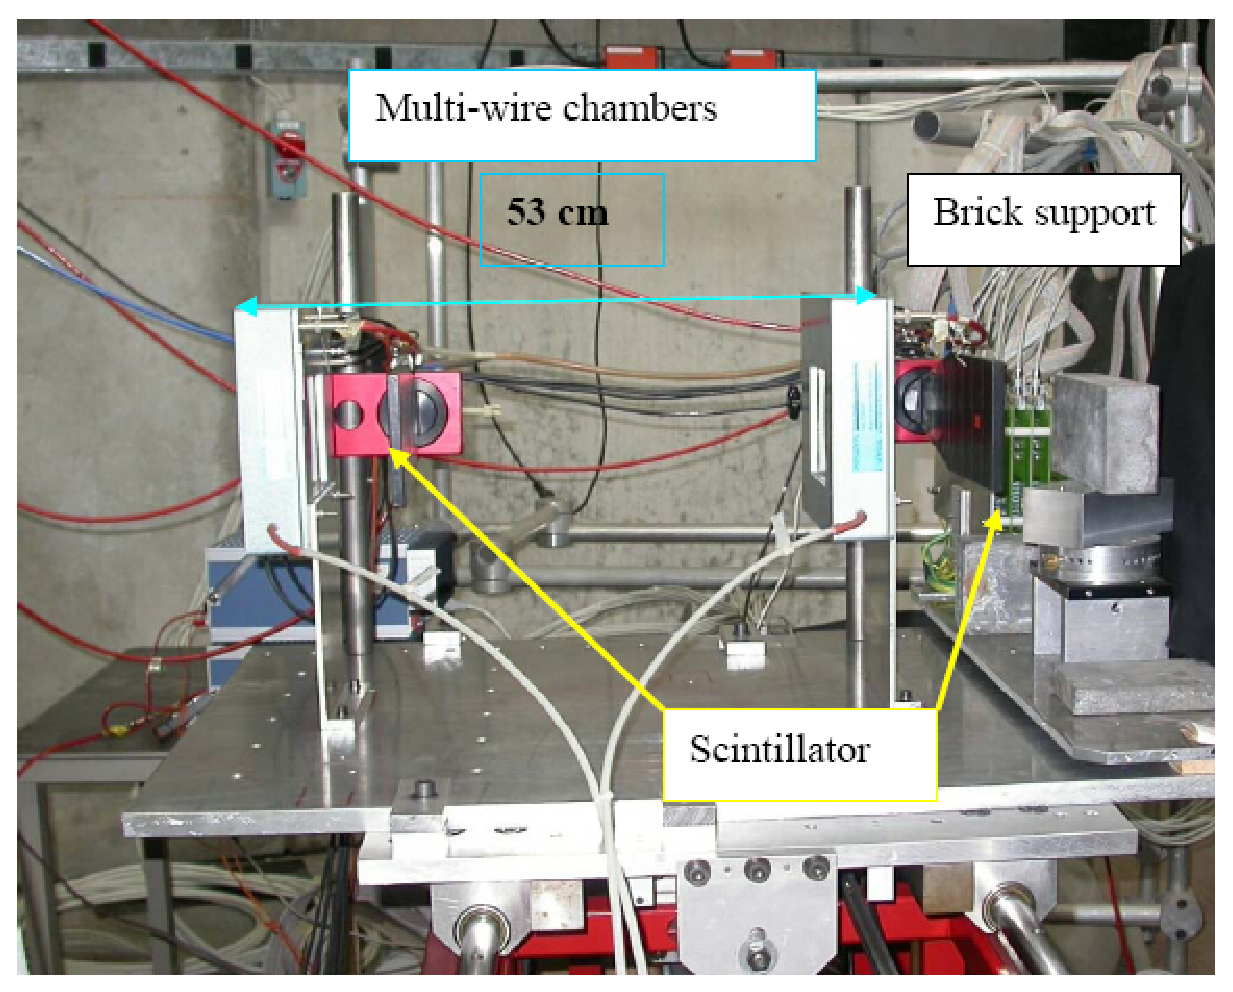
\includegraphics[width=90mm,height=90mm]{eps/testbeam.eps}
\end{center}
\caption{Apparato per le prove sul fascio nel novembre 2004.}
\label{fig:teastbeam}
\end{figure}

\begin{figure}[tbp]
\begin{center}
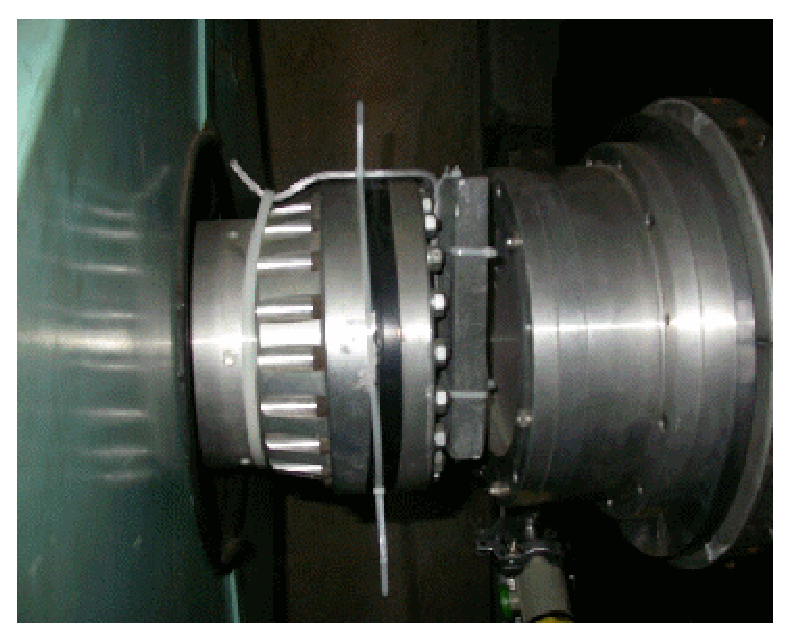
\includegraphics[width=90mm,height=90mm]{eps/shower.eps}
\end{center}
\caption{Assorbitore di elettroni.}
\label{fig:shower}
\end{figure}

L'apparato utilizzato per le prove su fascio � mostrato in figura
\ref{fig:teastbeam}.  Per ridurre la contaminazione di elettroni, un
assorbitore di piombo � stato posto prima dell'ultimo magnete
(fig. \ref{fig:shower}). Per misurare il flusso di particelle e la
loro direzione sono stati utilizzati due piani di scintillatori e
camere a deriva.

La densit� del fascio � stata posta a $0.1~ tracce/mm^2$ in maniera da
ottenere un giusto compromesso tra l'esigenza di lavorare in
condizioni di bassa densit�, quanto pi� vicine alle condizioni di
OPERA, e quella di accumulare un numero sufficiente di interazioni per
poter effettuare questo studio. Dopo l'esposizione, i CS sono stati
subito sviluppati, mentre il mattone � stato esposto a raggi cosmici
per circa $6h$, in modo da accumulare un numero sufficiente di tracce
passanti per consentire l'intercalibrazione tra i piatti. La densit�
di raggi cosmici nell'intervallo angolare di $-400 ~mrad \leq \theta
\geq 400~mrad$ � di circa $1$ traccia al $mm^2$. Successivamente il
mattone � stato disassemblato e i fogli di emulsioni sono stati
sviluppati.  Prima dello sviluppo viene impressa sulle emulsioni,
mediante l'uso di raggi X, una griglia utilizzata come riferimento
locale. Le posizioni delle tracce vengono misurate rispetto a questa
griglia, il che rende pi� semplice un successivo riposizionamento su
di esse.

Il mattone esposto al fascio � stato utilizzato per studiare la
procedura di Scan Back.

\section{Scansione dei CS e definizione del campione di predizioni}

Per definire il campione di tracce da inseguire, � stata effettuata
scansione su un'area di $25.9 ~cm^2$ nella parte centrale dei CS.

\begin{figure}[tbp]
\begin{center}
\includegraphics[width=90mm,height=90mm]{eps/cs_tx_ty.eps}
\end{center}
\caption{Distribuzione angolare delle tracce di base trovate nel foglio 
CS.}
\label{fig:cstxty}
\end{figure}

In figura \ref{fig:cstxty} � mostrata la distribuzione angolare delle
tracce di base nel primo CS. Si nota il picco angolare per
$\theta_X=50~mrad$ in corrispondenza del fascio di pioni. Nonostante il
refreshing, si � osservata una elevata densit� di tracce, rispetto a
quella desiderata. La densit� di tracce nei CS � di $26.2$ e $30.1$
tracce/$mm^2$, rispettivamente. Questa densit� di tracce si riduce
notevolmente se si considerano le coincidenze tra i due CS. Infatti
durante il viaggio in aereo il mattone non era assemblato, dunque le
tracce accumulate su un foglio di emulsione sono scorrelate da quelle
accumulate sugli altri fogli. Richiedendo per le tracce la coincidenza
dei due CS la densit� diventa 0.26 tracce/$mm^2$. Tale numero risulta
ancora essere troppo alto rispetto a quello desiderato. Il motivo �
che l'elevato fondo sui singoli fogli di emulsione porta a numerose
coincidenze casuali.

\begin{figure}[!tbp]
\begin{center}
\includegraphics[width=90mm,height=90mm]{eps/vtx09campione.eps}
\end{center}
\label{fig:vtx09campione}
\caption{Definizione del campione di predizioni per la procedura di
inseguimento.}
\end{figure}

\begin{figure}[tbp]
\begin{center}
\includegraphics[width=80mm,height=80mm]{eps/pred_ty_tx.eps}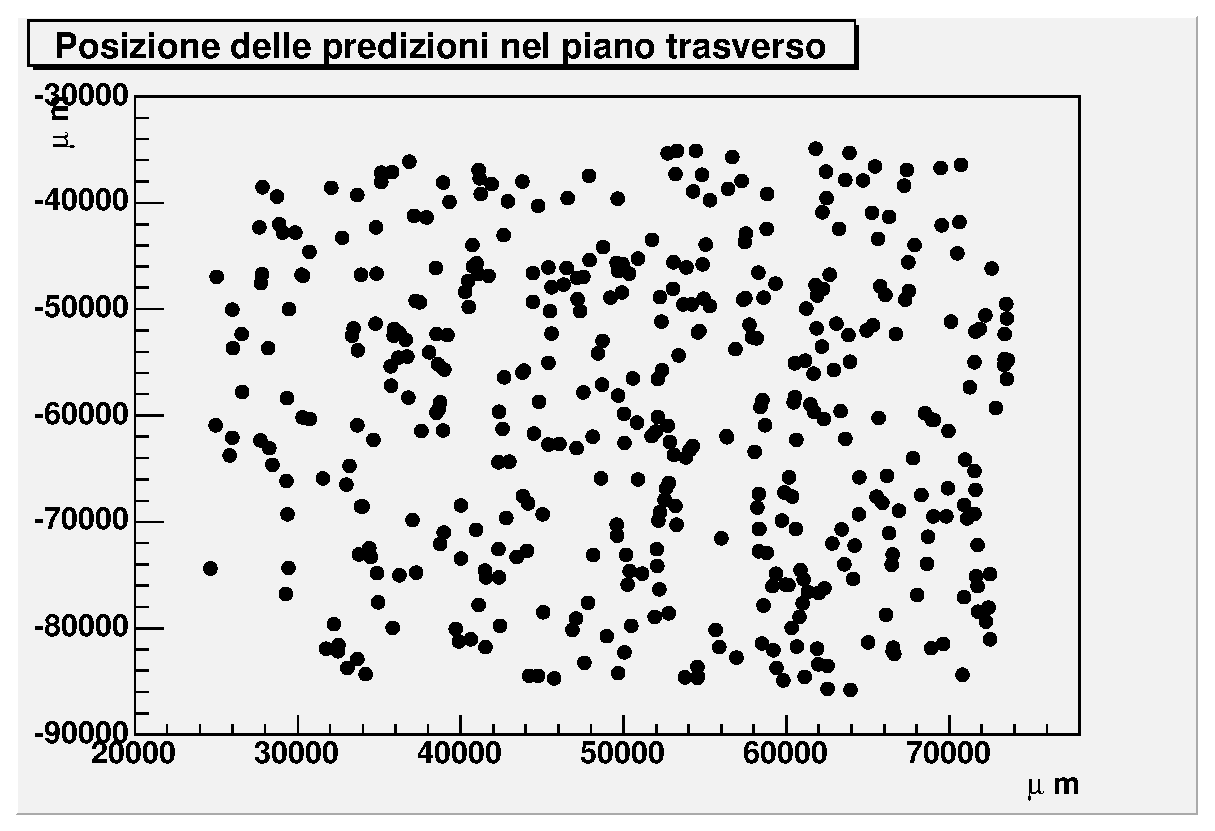
\includegraphics[width=80mm,height=80mm]{eps/pre_x_y.eps}

\end{center}
\caption{Distribuzione degli angoli  (sinistra) e delle posizioni (destra) delle predizioni.}
\label{fig:vtx09_tr3}
\end{figure}

Per una migliore purezza nella definizione del campione di predizioni,
si � ritenuto necessario utilizzare le tracce ricostruite oltre che
nei due CS anche nel primo piatto del mattone
(fig. \ref{fig:vtx09campione}). Intercalibrando e ricostruendo le
tracce nei tre piatti si ottiene una densit� di
$0.17~tracce/mm^2$. In figura \ref{fig:vtx09_tr3} � mostrata la
distribuzione angolare del campione, formato da $433$ tracce. Questo � il campione 
 utilizzato per lo Scan Back.


\section{Procedura di Scan Back}

Una volta definito il campione di tracce di partenza, pu� avere
inizio la procedura di Scan Back. In ordine temporale, per ogni foglio di
 emulsione le operazioni da effettuare in tale procedura sono:

\begin{itemize}
\item{Scansione di un'area centrale di $1\times1~cm^2$, utilizzata per
effettuare l'intercalibrazione del foglio con il precedente.}
\item{Determinazione della zona di scansione per ogni predizione, tenendo
conto della trasformazione affine tra i piatti.}
\item{Scansione della zona da analizzare per ogni predizione (1 campo).}
\item{Ricerca e selezione del miglior candidato per ogni singola predizione.}

\end{itemize}

Queste operazioni vengono effettuate su ogni foglio di emulsione, dal n. 2
al n. 56, procedendo a ritroso rispetto alla direzione del fascio.
 Le tracce trovate su un foglio costituiscono le predizioni
per il foglio successivo.

In seguito all'esposizione del mattone ai
raggi cosmici, in un'area di $1\times1~cm^2$ sono presenti circa un
centinaio di tracce oltre a quelle del fascio. Questo numero �
sufficiente ad intercalibrare i due piatti. Una volta determinati i
parametri di allineamento tra un foglio ed il precedente, questi
vengono usati per calcolare il punto a cui estrapolare le
predizioni. Attorno a questo punto, per ogni predizione, come primo
prova si � effettuata la scansione di un'area di circa
$1\times1~mm^2$ ( $3\times3$ campi visivi). In figura
\ref{fig:view3x3} sono mostrate le distribuzioni dei residui tra la
posizione della traccia predetta e le tracce trovate. Si osserva
chiaramente che il segnale � ben definito entro un intervallo di 100
$\mu m$. Sulla base di questo risultato � stato possibile scegliere
un'area di scansione corrispondente ad un solo campo visivo.

\begin{figure}[tbp]
\begin{center}
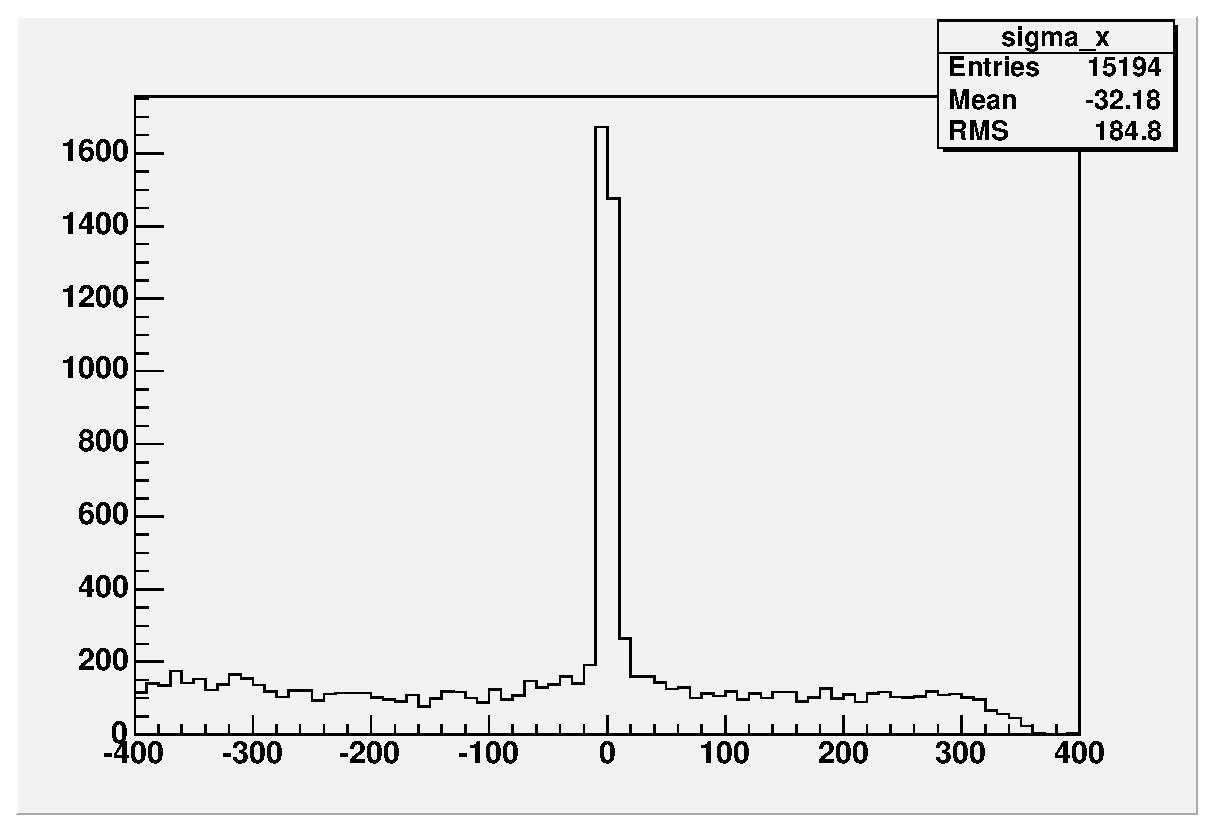
\includegraphics[width=60mm,height=80mm]{eps/view3x3x.eps}
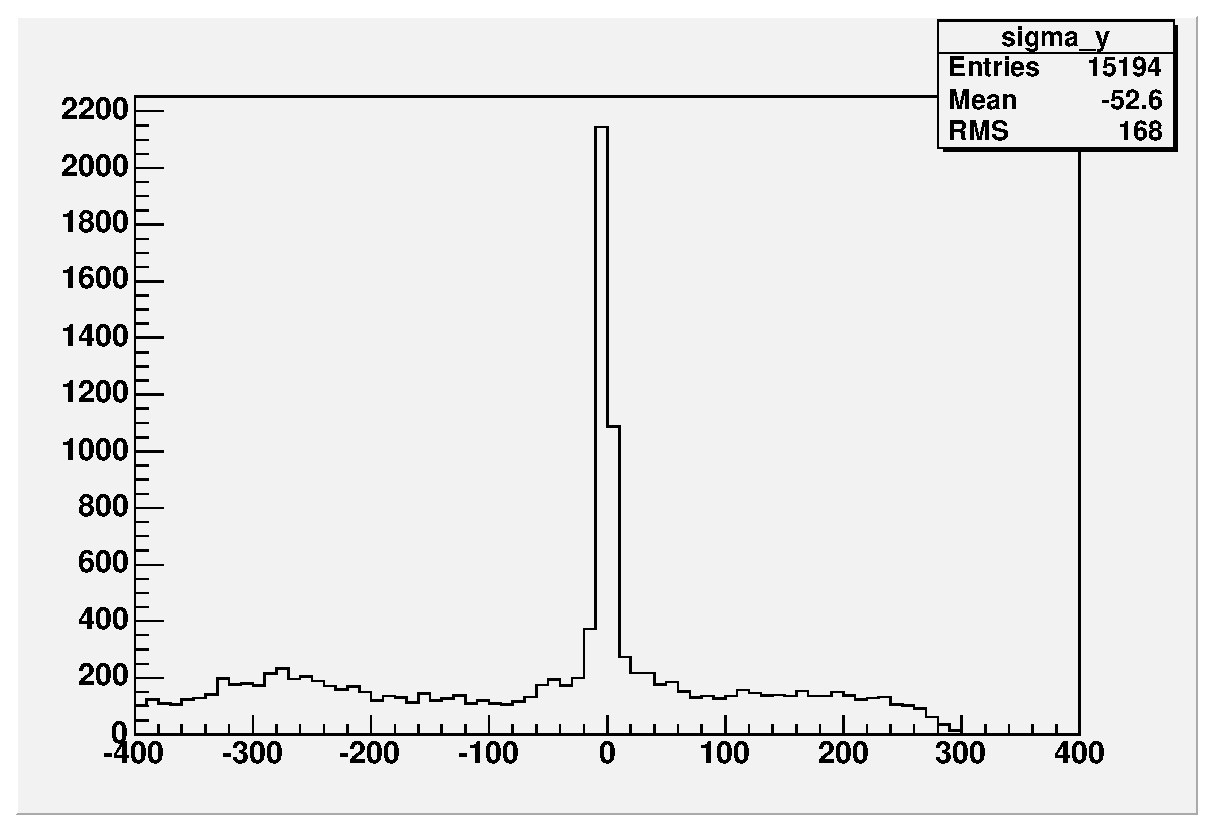
\includegraphics[width=60mm,height=80mm]{eps/view3x3y.eps}
\end{center}
\caption{Distribuzione della differenza in posizione 
tra  tracce predette e  candidate dopo una scansione di un'area di $1\times 1~mm^2$. Si nota che un'area corrispondente ad un campo di vista ($395\times300~\mu m^2$) \`e sufficiente a contenere il segnale entro oltre $3\sigma$. La distribuzione a sinistra \'e per la coordinata X, quella a destra Y espresse in $\mu m$.}
\label{fig:view3x3}
\end{figure}



\begin{figure}[tbp]
\begin{center}
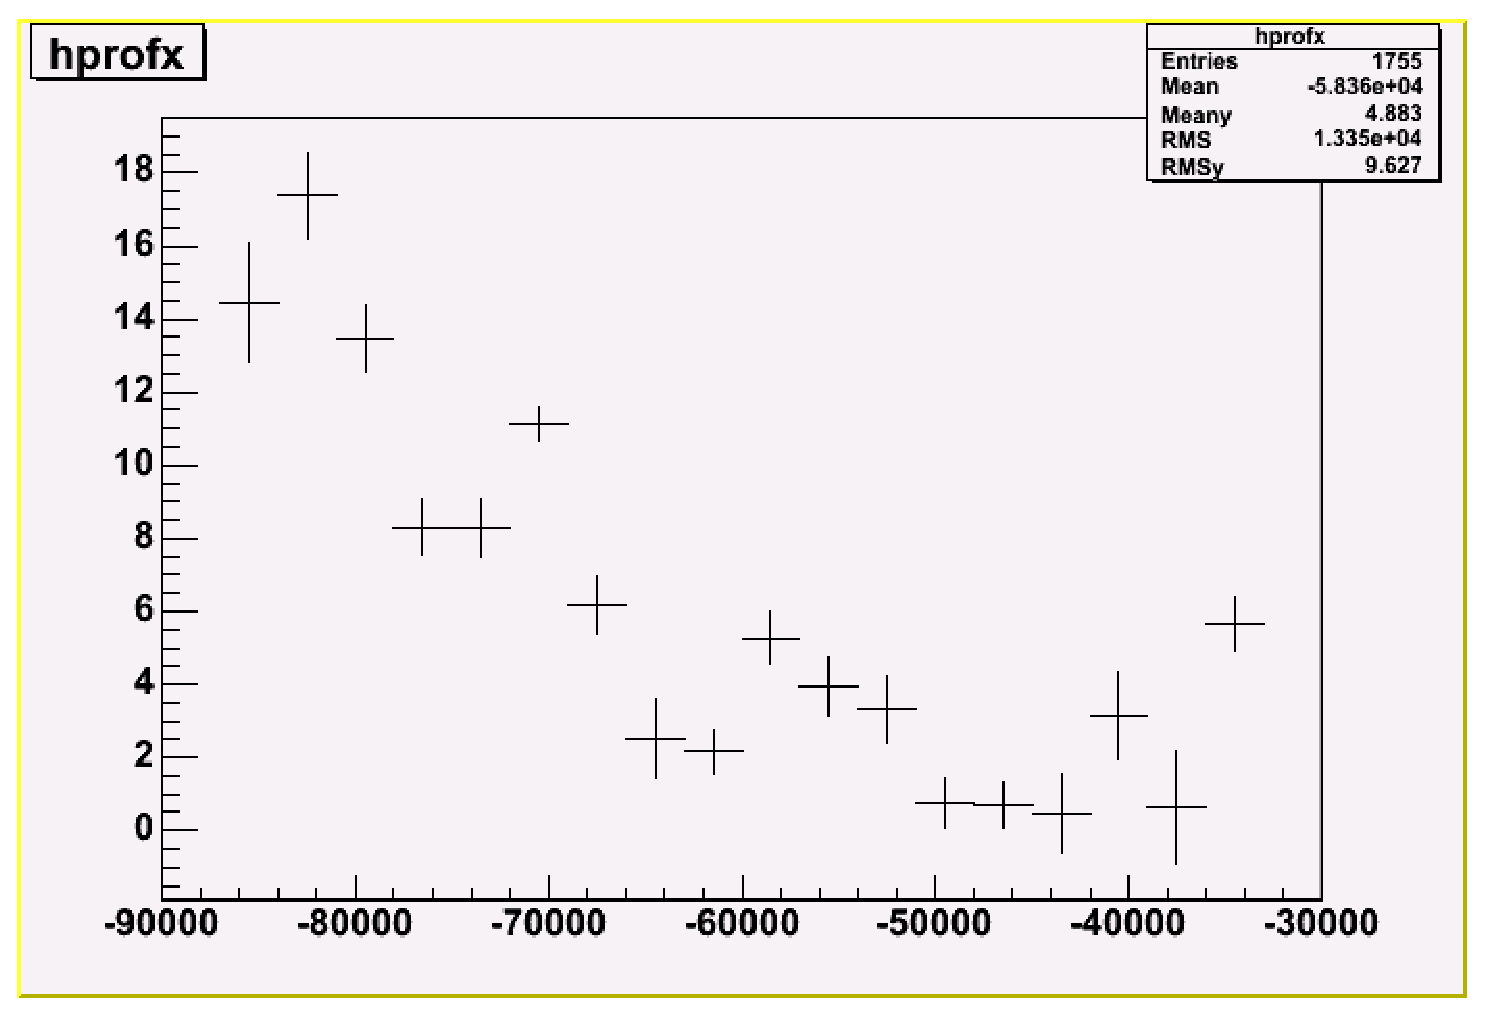
\includegraphics[width=70mm,height=80mm]{eps/profx.eps}
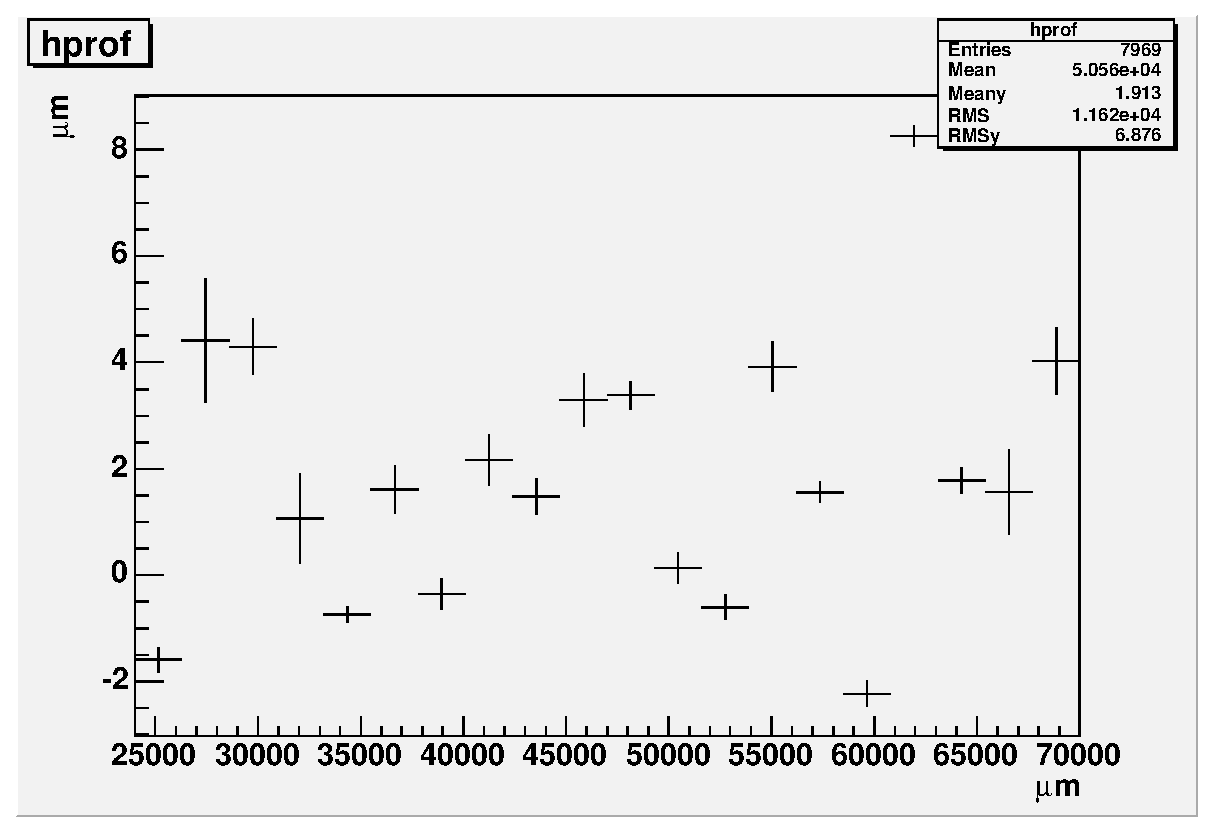
\includegraphics[width=70mm,height=80mm]{eps/dycorr.eps}
\end{center}
\caption{Differenza della coordinata X (sinistra)  di
predizione e candidati in funzione della coordinata stessa della
predizione. Il grafico a destra mostra la  stessa distribuzione dopo la correzione per l'offset.}
\label{fig:res_pos}
\end{figure}

La figura \ref{fig:res_pos} mostra che i residui in posizione hanno
una dipendenza dalla coordinata a causa di effetti locali non ben corretti dal primo allineamento. 
Infatti, la trasformazione affine tra i piatti � stata calcolata utilizzando
una zona centrale all'interno dell'area di 25.9 $cm^2$ in
esame. La dipendenza evidenziata viene parametrizzata e corretta, ottenendo
una distribuzione dei residui centrata a zero, come mostrato in
\ref{fig:res_pos}.



Per la ricerca e selezione del miglior candidato � stato definito un
estimatore $\chi^2$ nel seguente modo:

\begin{equation}
\chi^2=\frac{\Delta\theta^2_x}{\sigma^2_{\theta_x}}+
\frac{\Delta\theta^2_y}{\sigma^2_{\theta_y}}+\frac{\Delta
x^2}{\sigma^2_x}+\frac{\Delta y^2}{\sigma^2_y}
\end{equation}


dove:
\begin{itemize}
\item{$\Delta\theta_x$ e $\Delta\theta_y$ sono le differenze angolari
nelle due proiezioni tra la traccia predetta e quella trovata.}
\item{$\Delta X$ $\Delta Y$ sono le differenze in posizione nelle due
proiezioni tra la traccia predetta e quella trovata.}
\end{itemize}

I valori delle $\sigma$, sia in angolo che in posizione, sono stati
ottenuti da fit gaussiani delle distribuzioni dei residui delle
rispettive grandezze. Inoltre per quanto riguarda
$\sigma_{\theta_x},\sigma_{\theta_y}$ � stato tenuto conto della
degradazione angolare della risoluzione tramite la seguente
parametrizzazione:
\begin{equation}
\sigma(\theta)=\sigma(0)\cdot(1+4\cdot|\theta|)
\label{eq:sigmapar}
\end{equation}
Per ogni predizione si considera il candidato avente il $\chi^2$
 minore. La scelta viene effettuata solo sui candidati aventi
 $\chi^2\leq 6~(99.9\%)$. La distribuzione del  $\chi^2$ \`e mostrata
 in figura~\ref{fig:chi2pred}. In figura \ref{fig:sigmay} sono mostrate le
 distribuzioni dei residui in posizione e in angolo tra le tracce
 predette e quelle del miglior candidato.

\begin{figure}[tbp]
\begin{center}
\includegraphics[width=60mm,height=80mm]{eps/predchi2.eps}
\end{center}
\caption{Distribuzioni del $\chi^2$ dei candidati.}
\label{fig:chi2pred}

\end{figure}

\begin{figure}[tbp]
\begin{center}
\includegraphics[width=60mm,height=80mm]{eps/sigma_dx.eps}
\includegraphics[width=60mm,height=80mm]{eps/sigma_dtx.eps}
\end{center}
\caption{Distribuzioni dei residui in posizione  (a sinistra espresso in $\mu m$) ed in angolo
(a destra espresso in $rad$) tra le tracce predette ed il miglior candidato ottenuto con
l'estimatore $\chi^2$.}
\label{fig:sigmay}
\end{figure}

La valutazione dei tempi di scansione nella
procedura di Scan Back � importante in relazione al grande volume di dati
 che OPERA deve analizzare.

 La scansione della zona
necessaria all'intercalibrazione tra i fogli richiede circa 10
minuti. Per ogni predizione sono invece necessari circa 5 secondi, di
cui circa 4 sono impiegati per la ricerca della superfice
dell'emulsione. Il tempo totale impiegato per la ricerca delle 433
predizioni � dunque circa 36 minuti. Questo tempo, durante la
procedura di inseguimento, diminuisce gradualmente per il ridursi del
numero di predizioni.

La ricostruzione delle tracce acquisite e la
ricerca per ogni predizione del miglior candidato richiede qualche
minuto di processamento. Tuttavia questo tempo non si somma ai
precedenti. Infatti questa operazione pu� essere effettuata mentre
il microscopio sta analizzando la zona necessaria
all'intercalibrazione. Ad esempio, mentre si effettua la ricostruzione
delle tracce trovate nel foglio n .2 sul microscopio viene gi�
posizionato il foglio n. 3 ed inizia la scansione necessaria
all'intercalibrazione tra i fogli n. 2 e n. 3.

Il tempo totale per l'analisi di ogni foglio di emulsione � risultato
essere di circa 40 minuti. Gran parte (circa  80\%) del tempo
impiegato in questa procedura consiste nella ricerca delle superfici
dell'emulsione. Una possibile soluzione per evitare la rivelazione
delle superfici ad ogni predizione \`e quella di acquisire i diversi
strati di emulsioni partendo dall'esterno dell'emulsione e finendo
nella base. Il prezzo che si paga, per mantenere lo stesso
campionamento negli strati sensibili delle emulsioni \`e quello di
dover fare un numero di campionamenti totale pi\`u elevato. Tale
algoritmo \`e in fase di studio. 

\section{Definizione di vertice}
Se per una determinata predizione non viene trovato nessun candidato,
la traccia viene proiettata sul foglio successivo. Se il candidato non
viene trovato per un numero di fogli consecutivi superiore a tre, si
assume che la traccia si sia arrestata ed essa non viene ulteriormente
inseguita nei fogli successivi. Il taglio a tre segmenti tiene conto
della efficienza di tracciamento. Infatti essendo l'inefficienza pari
a circa il 10\%, la richiesta dell'assenza di tre segmenti per
definire una traccia che si ferma corrisponde  a tollerare  un'inefficienza di
circa lo 0.1\%. 

\begin{figure}[tbp]
\begin{center}
\includegraphics[width=120mm,height=80mm]{eps/plpred.eps}
\end{center}
\caption{Distribuzione del numero di predizioni al variare del numero
del foglio.}
\label{fig:plpred}
\end{figure}
Utilizzando questa procedura, il campione iniziale di 433 predizioni �
stato inseguito fino al foglio 56, che come si � detto � quello pi� a
monte.  In figura \ref{fig:plpred} viene mostrato l'andamento della
distribuzione del numero di predizioni in funzione del numero di
foglio. Il numero di predizioni mostra un calo pi� marcato nei fogli
pi� a valle rispetto alla direzione del fascio. Questo \`e dovuto alla
purezza delle predizioni che \`e evidentemente ancora scadente, pur
avendo richiesto la triplice connessione tra i segmenti ricostruiti
nei CS e quelli del primo piatto del brick come tracce di partenza. La
richiesta di tre segmenti consecutivi all'interno del brick
normalmente riduce drasticamente (al di sotto dell'1\%) le connessioni
casuali a tutto vantaggio della purezza. Nel caso del CS in
questione, il salto di 4.7~mm tra i fogli CS e il primo piatto di
brick fa s\`{\i} che le accuratezze degli allineamenti siano pi\`u
scadenti e quindi le coincidenze casuali aumentino. Si noti che questi
CS sono stati attaccati dall'altra parte del brick rispetto alla
posizione prevista nell'esperimento. Questo \`e stato necessario a
causa dei supporti dei changeable sviluppati per prova e non adatti ad
essere montati nella posizione nominale.

\section{Analisi al vertice}
Come detto nela sezione precedente, la scomparsa di una traccia  
 costituisce un possibile vertice di
interazione. La lastrina di piombo immediatamente a monte dell'ultimo
foglio di emulsione dove si \`e vista la traccia viene definita come
la lastrina di interazione. Avendo inseguito una sola traccia, non
siamo in grado di definire e studiare il vertice di interazione. A tal
fine \`e quindi necessario fare delle acquisizioni aggiuntive in un
volume intorno al punto di vertice. Il volume viene definito da una
superficie di $5\times 5~mm^2$ ripetuta per 8 lastre, 4 a monte e 4
a valle del foglio di piombo dove \`e presumibilmente avvenuta
l'interazione.  La figura~\ref{fig:stop} mostra il volume fiduciale
analizzato nell'analisi al vertice.
\begin{figure}[tbp]
\begin{center}
\includegraphics[width=60mm,height=80mm,angle=90]{eps/stop.eps}
\end{center}
\caption{Schema della determinazione del volume per la scansione al vertice.}
\label{fig:stop}
\end{figure}

Dopo la scansione delle 8 zone nei piatti consecutivi, si procede
all'analisi offline dei dati. Prima vengono ricostruite le tracce di
base in ciascun foglio e poi si procede all'allinemento delle 8
lastre. L'allineamento viene mediamente effettuato con circa 20 tracce
passanti in una superficie di $25~mm^2$, oltre a quelle
dell'interazione in questione. 

Tutte le tracce ricostruite vengono divise in due categorie:
tracce passanti, ovvero quelle che attraversano tutto il volume
fiduciale senza fermarsi al suo interno, e tracce che si fermano
all'interno del volume. Prima di definire la traccia come fermatasi all'interno del volume si procede
 a effettuare la procedura cosiddetta di {\emph{relink}}, ovvero si cercano eventuali segmenti che possano costituire il prolungamento della traccia. 
Solo queste ultime partecipano alla successiva
procedura di ricostruzione del vertice basata sul parametro di impatto.

Un vertice viene definito dalla combinazione di almeno due tracce aventi una probabilit\`{a} del fit del vertice di almeno il $5\%$, secondo un algoritmo sviluppato per la ricostruzione dei vertici nell'esperimento HERA-B e opportunamente riadattato al caso dei dati in emulsione \cite{HERAB}.

\begin{figure}[tbp]
\begin{center}
\includegraphics[width=60mm,height=80mm]{eps/cap4/impatto.eps}\includegraphics[width=60mm,height=80mm]{eps/cap4/impatto_theta.eps}

\end{center}
\caption{Distribuzione del parametro di impatto delle tracce rispetto al vertice (sinistra). Nel grafico a destra \`{e} mostrato l'andamento del parametro di impatto in funzione dell'angolo della traccia.}
\label{fig:impatto}
\end{figure}


La figura \ref{fig:impatto} mostra la distribuzione del parametro di impatto delle tracce rispetto al vertice. Come si pu\`{o} notare, tale distribuzione suggerisce un taglio a $10~\mu m$. Tale distribuzione dipende poco dall'angolo della traccia come mostrato nel grafico  destro della figura \ref{fig:impatto}.

A causa della gi\`{a} menzionata impurit\`{a} delle predizioni nei primi fogli di emulsione e per poter avere un volume fiduciale nominale, consideriamo in questa analisi come campione di normalizzazione le sole predizioni che si sono fermate a partire dal piatto 4 e fino al 52. Data la lunghezza di interazione nel piombo (circa $17~cm$) il tasso di interazioni di pioni atteso \`{e} di circa il $25\%$. Su 341 predizioni di partenza al piatto 4, se ciascuna corrispondesse ad una interazione primaria o al primario stesso, ci aspetteremmo circa 85 interazioni fino al piatto 52. Sappiamo per\`{o} che alcune di esse inevitabilmente provengono da interazioni secondarie di particelle cariche o neutre prodotte da un interazione primaria. 


\begin{figure}[tbp]
\begin{center}
\includegraphics[width=60mm,height=80mm]{eps/cap4/parente.eps}

\end{center}
\caption{Angoli delle tracce da cui si originano i vertici.}
\label{fig:parente}
\end{figure}


Le 119 tracce che si sono fermate tra i piatti 4 e 52 sono state classificate come mostrato in tabella \ref{tab:vertici}. Di esse, 46 danno origine a un vertice con due possibili topologie: se ci sono solo due tracce, una \`{e} quella di scan-back e l'altra \`{e} la traccia primaria; se le tracce sono almeno tre, una \`{e} comunque primaria. In figura \ref{fig:good} \`e mostrato il display di un vertice di interazione ricostruito. Si vedono 5 tracce secondarie inclusa la traccia di scan-back dipartirsi dal vertice di interazione preceduto dalla traccia progenitrice, che ha un angolo compatibile con quello del fascio di pioni utilizzato. Il vertice di interazione si origina nella lastra di piombo compresa tra i piatti 38 e 39, 10 $\mu m$ a valle della lastra 39. Di questi 46 vertici, 36 hanno almeno 2 tracce con parametro di impatto rispetto al vertice inferiore a $10~ \mu m$ per entrambe. Le altre 10 saranno oggetto di  ulteriori studi compreso l'ispezione visiva al microscopio. 

20 tracce sono risultate essere passanti. Ci\`{o} \`{e} indice di inefficienze (circa $17\%$) nella procedura di localizzazione del foglio di vertice da imputare a distorsioni locali delle lastrine di emulsione. 21 tracce si fermano all'interno del volume fiduciale senza che alcuna di esse le preceda o le accompagni nell'interazione. 22 tracce mostrano una topologia di tipo {\emph{a gomito}}, ovvero sono precedute a monte del piatto di arresto da una traccia che forma con essa un angolo inferiore a $30~mrad$. Tale topologia \`{e} tipica delle interazioni elastiche dei pioni. Infine 6 tracce mostrano una traccia progenitrice che evidenzia diverse deflessioni. 4 volumi non sono stati analizzati per problemi di  allineamento, la cui soluzione necessiter\`{a} nuove acquisizioni.

\begin{table}
\begin{center}
\begin{tabular}{||c|c||}
\hline
\hline
Categoria &Numero di eventi\\
\hline
Vertici a due  o pi\`{u} tracce & 46\\
\hline
Traccia passante& 20\\
\hline
Traccia fermatasi senza vertice& 21\\
\hline
Kink & 22\\
\hline
Deflessioni multiple& 6\\
\hline
Problemi di allineamento& 4\\
\hline
Totale &119\\
\hline
\end{tabular}
\label{tab:vertici}
\end{center}
\end{table}



Il numero totale di possibili interazioni rivelate \`{e} pertanto formato dalla 
prima, quarta e quinta categoria di eventi per un totale di 74 
interazioni, da confrontare con le circa 85 attese. Si noti che la
 stima delle 85 tracce attese contiene delle approssimazioni normalmente
 applicabili alla procedura di {\emph{Follow Down}} e non a quella di {\emph{Scan Back}}. 
Pertanto essa \`{e} da considerare come un limite superiore alle interazioni attese.



\begin{figure}[tbp]
\begin{center}
\includegraphics[width=60mm,height=80mm]{eps/cap4/good.eps}

\end{center}
\caption{Display di un vertice di interazione ricostruito.}
\label{fig:good}
\end{figure}







%\chapter{Brick13  e Dummy}


Durante il test Beam di novembre 2004 di sono effettuati esposizioni a fasci di pioni ad alta densit�  di $8GeV$, per lo studio sitematico delle problematiche realative alla connessione CS al Brick e alla ricostruzione di vertici di interazioni. Per lo studio dei CS � stato esposto un  Brick, denominato brick13. IL brick13  � formato da 56 lastrine di emulsione intervallate da lastre di piombo. Di queste 56 solo le ultime 3, quelle pi� a valle rispetto alla direzione del fascio, sono state sviluppate. I due CS sono stati dapprima inseriti in una busta di alluminio, la quale viene saldata termicamente, dopo aver effettuato il vuoto.
I due CS sono connessi al brick mediante il portachangebale (vedi figura \ref{fig:brick13}. Il brick e' stato esposto al fascio di pioni con angolo di incidenza $320mrad~~100mrad~~e -150mrad$ nella proezione $X$ (fig. \ref{fig:b13txty}). In tabella \ref{table:brick13D} sono riportati il numero di trigger misurato dagli scintillatori per i vari angoli di incidenza.



\begin{figure}[!tbp]
\begin{center}
\includegraphics[width=90mm,height=90mm]{eps/brick13.eps}
\end{center}
\label{fig:brick13}
\caption{Schema brick13 }
\end{figure}



\begin{table}
\begin{center}
\begin{tabular}{||c|c|c|c||}
\hline
\hline
Brick &-150mrad& 100mrad&320mrad\\
\hline
\#13& 57398& 56734&63083\\
\hline
\end{tabular}
\label{table:brick13D}
\end{center}
\end{table}


Per le 5 lastrine del brick13 (2CS+3brick) si  � effettuato una'area di scansione di $\sim 80cm^2$ in modo da avere uno studio della connessione e planarit� su tutta la superfice e studiare eventuali effetti di bordo.

Prima della procedura di intercalibrazione occorre determinare la distanza tra le  superfici della lastrina CS2 e PL01. Questa distanza non � nota con molta precisione. Quindi si  � sviluppato un tool per la determinazione di questa distanza utilizzando le traccie a grande angolo del fascio. Si sono effettuati varie iterazioni , in modo da tener conto sia  delle rototraslazione per ogno varizione della  distanza tra i due piatti.
Il valore ottenuto da questa procedura  di� $4.7mm$. Dopo questa procedura � stato possibile effettuare la procedura di intercalibrazione dei vari piatti i, in modo da avere una misura del didiallinemanto tra le varie lastrine. In tabella \ref{table:aff} sono riportate le trasformazioni affini, riferite al CS1, dei vari piatti ottenute dalla procedura di intercalibrazione. Mentre in tabella \ref{table:aff1} sono riporrtate le trasfromazioni affini di un piatto rispetto ad un altro.

\begin{table}
\begin{center}
\begin{tabular}{||c|c|c|c|c|c|c|c||}
\hline
Piatto&Z&A11&A12&B1&A21&A22&B2\\
\hline
CS1&-7900&1.0&0.0&0.0&1.0&0.0&0.0\\
\hline
CS2 &-7600&0.999963&-0.009357&0.009699&0.9999897&-35.041355&-11.182884\\
\hline
PL01&-2600&1.000682&-0.018341&0.018584&1.0026976&78.772865&-1039.353271 \\
\hline
PL02& -1300&1.000722&-0.007328&0.008518&1.003592&-72.062424&-956.398071\\
\hline
PL03& 0&1.000836&-0.007328&0.008518&1.003592&-74.062424&-956.398071\\
\hline

\end{tabular}
\end{center}
\caption{Trasformazioni affini rispetto al CS}
\label{table:aff}
\end{table}




\begin{table}
\begin{center}
\begin{tabular}{||c|c|c|c|c|c|c|c||}
\hline
Piatto&Z&A11&A12&B1&A21&A22&B2\\
\hline
CS2 &-7600&0.999963&-0.009357&0.009699&0.9999897&-35.041355&-11.182884\\
\hline
PL01&-2600&1.000682&1.000765&-0.008784&1.002806&94.667931&-1030.047852 \\
\hline
PL02& -1300&1.000255&0.004211&-0.003501&1.000555&-55.183800&23.849262\\
\hline
PL03& 0&1.000010&0.006728&-0.006572&1.000162&-67.190315&58.578827\\
\hline
\end{tabular}
\end{center}
\caption{Trasformazioni affini rispetto al piatto precedente}
\label{table:aff1}
\end{table}

           

Dalla tabella \ref{table:aff1} si nota che il disallineamento tra i due CS �
 contenuto in poche decine di micron, dello stesso ordine di grandezza del disallineamento tra le lastre del brick. Mentre per quanto riguarda il CS2 e PL01 abbiamo un disallineamento di poco pi� $1mm$ solo nella direzione $Y$. 


\begin{figure}[!tbp]
\begin{center}
\includegraphics[width=90mm,height=90mm]{eps/peak_b13.eps}
\end{center}
\label{fig:b13txty}
\caption{Distribuzione angolare  }
\end{figure}


Si � anche studiata l'efficienza di tracciamento per i vari angoli per il piatto PL03. In tabella \ref{table:eff} sono riportati i valori ottenuti per i vari angoli. I valori ottenuti sono confrontabili  con quelli ottenuti in tabella \ref{table:eff}, oltretutto tenendo conto della gap di $4.7mm$ tra il CS2 e PL01.



\begin{table}
\begin{center}
\begin{tabular}{||c|c|c|c|c||}
\hline\hline
Angolo&tx(rad) &eff\\
\hline
P00& 0.320&$85.9 \pm0.63$\\
\hline
P01&0.100&$91.6 \pm 0.45$\\
\hline
P02&-0.160&$88.9 \pm 0.65$\\
\hline\hline
\end{tabular}
\label{table:effcs}
\caption{Misura di efficienza di ricotruzione a vari angoli. }
\end{center}
\end{table}






{\Huge Profile}



\begin{figure}[tbp]
\begin{center}
\includegraphics[width=90mm,height=90mm]{eps/CStx0.eps}
\end{center}
\caption{Differenza angolare nella proezione X $\theta=320mrad$  }
\end{figure}

\begin{figure}[tbp]
\begin{center}
\includegraphics[width=90mm,height=90mm]{eps/CStx1.eps}
\end{center}
\caption{Differenza angolare nella proezione X $\theta=100mrad$  }
\end{figure}

\begin{figure}[tbp]
\begin{center}
\includegraphics[width=90mm,height=90mm]{eps/CStx2.eps}
\end{center}
\caption{Differenza angolare nella proezione X $\theta=-150mrad$  }
\end{figure}

\begin{figure}[tbp]
\begin{center}
\includegraphics[width=90mm,height=90mm]{eps/CSty.eps}
\end{center}
\caption{Differenza angolare nella proezione X $\theta=-150mrad$  }
\end{figure}

\begin{figure}[tbp]
\begin{center}
\includegraphics[width=90mm,height=90mm]{eps/cs1_2_b13.eps}
\end{center}
\caption{Planarita' dei due cs sulla tutta la superfice}
\end{figure}

\section{Connessione due CS , brick dummy}



\chapter*{Conclusioni}
\addcontentsline{toc}{chapter}{Conclusioni}

L'esperimento OPERA nasce per misurare la probabilit\`a di oscillazione
$\nu_{\mu} \rightarrow \nu_{\tau}$ nella regione dei parametri indicata
dagli esperimenti con i neutrini atmosferici. Esso si basa sulla
rivelazione del vertice di produzione e di decadimento del leptone $\tau$,
resa possibile dalla risoluzione sub-micrometrica delle emulsioni nucleari
utilizzate come sistema tracciante. Per ottenere un bersaglio con la elevata massa
che \`e necessaria, data la bassissima sezione d'urto dei neutrini e il flusso ridotto a
 causa della distanza dalla produzione, viene usata la tecnica nota come Emulsion
Cloud Chamber. In essa, i fogli di emulsione si alternano a sottili  lastre di piombo che
sostanzialmente forniscono la massa del bersaglio per il neutrino.

Le emulsioni nucleari negli ultimi 20 anni hanno conosciuto una
rinascita grazie allo sviluppo di microscopi automatici ad alta
velocit\`a che hanno reso completamente automatica quella che un tempo
era un'analisi esclusivamente visiva e pertanto faticosissima e lenta
al microscopio. Un progetto di ricerca mirato allo sviluppo di
microscopi di nuova generazione che consentissero l'analisi di
lastre di emulsioni ad altissima velocit\`a (circa 20~cm$^2$/h) \`e
partito nel 2001 e ha conseguito recentemente i risultati prefissati
in termini di velocit\`a, efficienze e purezze di tracciamento. 

Collegato a questo progetto e parallelamente ad esso, \`e in fase di
sviluppo il software di ricostruzione e analisi dei dati provenienti dal
sistema di scansione ad alta velocit\`a realizzato. In particolar modo, il
tracciamento di particelle al minimo di ionizzazione in Emulsion Cloud
Chamber \`e stato affrontato con successo mentre \`e ancora in fase di
sviluppo la procedura di localizzazione, ricostruzione e analisi dei
vertici. La tesi \`e stata mirata a tali studi. Una Emulsion Cloud
Chamber, costituita da 56 lastrine, \`e stata esposta ad un fascio di
pioni di 8 GeV prodotti dall'acceleratore PS al CERN di Ginevra.

Partendo dalle lastre pi\`u a valle relativamente al fascio di pioni, le
tracce ricostruite sono state seguite nelle lastre pi\`u a monte fino a
definire un possibile vertice di interazione dalla scomparsa su tre lastre
consecutive della traccia cercata.  Dopo aver definito un possibile
vertice, questo viene validato da una scansione aggiuntiva in cui viene
analizzato un volume di emulsione intorno al punto di arresto ottimizzato
in modo da massimizzare l'efficienza di ricostruzione di vertici al suo
interno. La procedura \`e stata applicata a 433 tracce localizzate e  misurate
nelle lastrine pi\`u a valle e inseguite per tutte le 56 lastre. Sono
stati determinati 119 punti di arresto e, intorno ad esso,
analizzati volumi di $5 \times 5$~mm$^2$ per 8 lastre consecutive.

\`E stata messa a punto, automatizzandola, la procedura di
inseguimento delle tracce in lastre successive, con un'analisi di
$\chi^2$. I punti di arresto delle tracce sono stati definiti  dalla
mancanza del segmento cercato in tre lastre consecutive, tenendo
opportunamente conto dell'inefficienza del tracciamento. Dopo la
scansione aggiuntiva nel volume circostante il punto di arresto, \`e stata
sviluppata un'analisi basata sulla tecnica del parametro di impatto, per
selezionare vertici a due o pi\`u tracce. Alcuni di questi
vertici sono anche stati validati da un'ispezione visiva al
microscopio della lastra precedente e successiva a quella di piombo
dove l'interazione \`e avvenuta. 


Tale analisi costituisce un primo importante passo verso la ricostruzione 
completamente automatizzata di vertici di interazione nella Emulsion Cloud Chamber 
dell'esperimento OPERA, secondo una procedura complessa e delicata.
Essa necessita, in particolare, di ulteriore perfezionamento dei criteri di selezione
 per ottimizzare l'efficienza di ricostruzione.

Gli algoritmi sviluppati e messi a punto con interazioni di pioni fanno
parte nel software di ricostruzione dei dati di emulsioni e saranno
interfacciati con il sistema di database in fase di sviluppo. La
metodologia messa a punto e gli algoritmi sviluppati saranno utilizzati
con i primi fasci di neutrini disponibili, in prove sul fascio NuMI al Fermilab
nel corso del 2005 e durante la presa dati dell'esperimento OPERA a
partire dal 2006.

\chapter*{Ringraziamenti}

Desidero ringraziare il Gruppo di Fisica del Neutrino di Napoli per il sostegno datomi in questi mesi.

Ringrazio il Prof. Paolo Strolin per avermi concesso la possibilit\`a di fare questa esperienza. La sua dedizione alla ricerca e al lavoro saranno sempre per me un esempio da seguire nella mia carriera professionale.


Ringrazio il Dott. Giovanni De Lellis per i suoi consigli, il sostegno e l'esperienza che ha messo a mia disposizione. Merita tutta la mia stima, oltre che per le sue conoscenze, per la sua grande umanit\`a e disponibilit\`a.

In particolare ringrazio il Dott. Francesco di Capua per avermi  aiutato nei momenti di panico e sconforto. Ringrazio i Dottori Danilo Coppola, Alberto Marotta, Ciro Pistillo, Luca Scotto per il loro aiuto e per essere stati sempre pronti ad offrirmi il loro supporto scientifico e morale. 

Ringrazio la mia famiglia per avermi dato la possibilit\`a di raggiungere uno degli obiettivi pi\`u importanti della mia vita. 

Ringrazio Fiorella per essermi stata vicino in questo cammino, per la sua pazienza e il suo supporto nei momenti difficili.


Ringrazio vivamente Francesco, Rosario e Gennaro per i loro consigli e chiaccherate nei tempi passati e presenti.


\addcontentsline{toc}{chapter}{\protect{Bibliografia}}
\begin{thebibliography}{99}


\bibitem{Chadwick}{J. Chadwick, Verh. d. D. Phys. Ges. {\bf{16}} (1914) 383.}
\bibitem{Ellis}{C.D. Ellis and W.A. Worster, Proc. Royal Soc. {\bf{A117}} (1927) 109}
\bibitem{Fermi}{E. Fermi, Z. Physik  {\bf{88}} (1934) 161}
\bibitem{Bethe}{H. Bethe, H. Peierl, Nature {\bf{133}} (1934)  532 .}
\bibitem{Donut} K. Hoshino (DONUT Collaboration), {\em Result from DONUT: First direct evidence for tau-neutrino},  8th Asia Pacific Physics Conference (APPC 2000), Taipei, Taiwan, 7-10 Aug 2000.
\bibitem{Lee}{T.D. Lee e C.N. Yang, Phys. Rev. {\bf{104}} (1956) 254}

\bibitem{Wu}{C.S. Wu, Phys. Rev. {\bf{105}}  (1957) 1413}
\bibitem{Majorana}{E. Majorana, Nuovo Cimento {\bf{14}} (1937) 171}
\bibitem{Bohem}{F. Boehm e P.Vogel, {\emph{Physics of massive neutrinos}}, Cambridge University Press(1987)}
\bibitem{ReinesCowan}{F. Reines, C.L. Cowan, Phys. Rev. {\bf{90}}, (1953), 492.}
\bibitem{SK} S.~Fukuda et al., Phys. Lett. B539 (2004) 179.
\bibitem{sno}  Q. R. Ahmad et al., Phys. Rev. Lett. 92 (2004) 181301.
\bibitem{ccsno} Q. R. Ahmad et al., Phys. Rev. Lett. 87 (2001) 071301.
\bibitem{ncsno} Q. R. Ahmad et al., Phys. Rev. Lett. 89 (2002) 011302. 
\bibitem{chooz} M.~Apollonio et al., Phys. Lett. B466 (1999) 415. 
\bibitem{kamland} K. Eguchi et al., Phys. Rev. Lett. 90 (2003) 021802.
\bibitem{lma} G.L. Fogli et al., Phys. Rev. D66 (2002) 093008. 
\bibitem{lma12} G.L. Fogli et al., presentato a Physics in Collision
2003, hep-ph/0310012.
\bibitem{SKa} T.~Kajita e Y.~Totsuka, Rev. Mod. Phys. 73 (2001) 85. 
\bibitem{soudan2} W.W.~Allison et al., Phys. Lett. B449 (1999) 137.
\bibitem{macro} M. Ambrosio et al., Phys. Lett. B517 (2001) 59.
\bibitem{k2k} M.H.~Ahn et al., Phys. Rev. Lett. 90 (2003) 041801. 
\bibitem{clorine} R.~Davis et al., Atrophys.~J. 496 (1998) 505.
\bibitem{gallium} W.~Hampel et al., Phys. Lett. B447 (1999) 127.

\bibitem{Davis}{Raymond Davis Jr., Phys. Rev. {\bf{96}}  (1953)  492}
\bibitem{MSS}{ J. N. Bachcall, M. H. Pinsonneault e S. Basu  , Astrophys. J.  {\bf{555}} (2001)}
\bibitem{Homestake}{R. Davis, Jr., D.S. Harmer e K.C. Hoffman, Phys. Rev. Lett. {\bf{20}}  (1958)  1205}
\bibitem{SNO}{Q.R. Ahmad, Phy. Rev. Lett. {\bf{89}}  (2002)}
\bibitem{LSND}{ http://www.neutrino.lang.gov/LSND/}
\bibitem{charm}{Opera Collaboration, "OPERA:{\emph{An appearance experiment to search for $\nu_\mu\rightarrow \nu_\tau$ oscillations in the CNGS beam.}} Experimental proposal", CERN-SPSC-2000-028}.



%cap2
%\bibitem{CNGS}{Bailey, R. et al. (1999). CERN-SL/99034 (DI); INFN/AE -99/05}

%NuMI
\bibitem{B1} K. Bourkland, K. Roon and D. Tinsley (NuMI Collaboration),{\emph{ 205-kA pulse power supply for neutrino focusing horns}}, FERMILAB-CONF-02-122-E, presented at the Power Modulator Conference, Hollywood, California, Jul 1-3, 2002.

%MINOS
\bibitem{B2} E. Buckley-Geer (MINOS Collaboration), \emph{Status of the MINOS experiment}, \textbf{503}  122 (2001).

%CNGS
\bibitem{B3} M. Nakamura, {\emph{Status of the CNGS experiment}} \textbf{111}  175 (2002).

%ICARUS
\bibitem{B4} J. Rico (ICARUS Collaboration), Status of ICARUS, hep-ex/0205028.

%OPERA
\bibitem{B5} D. Duchesneau (OPERA Collaboration), {\emph{The CERN - Gran Sasso neutrino program}}, \textbf{C0209101}, TH09 (2002),  (arXiv:hep-ex/0209082).

\bibitem{pione} C.M.G. Lattes, H. Muirhead, G.P.S. Occhialini and C.F. Powell, Nature {\bf{159}} (1947) 585. 
\bibitem{jpsi1} J.J. Aubert et al., Phys. Rev. Lett. {\bf{33}} (1974) 1404.
\bibitem{jpsi2} J.E. Augustin et al., Phys. Rev. Lett. {\bf{33}} (1974) 1406.
\bibitem{jpsi3} C. Bacci and et al., Phys. Rev. Lett. {\bf{33}} (1974) 1408 [Erratum-ibid. {\bf{33}} (1974) 1649]
\bibitem{Niu}  K. Niu, E. Mikumo e Y. Maeda, {\em A possible decay in flight of a new type particle},
Prog. Theor. Phys. \textbf{46} (1971) 1644
\bibitem{beauty}  S. W. Herb et al., Phys. Lett. {\bf{39}} (1977) 252
\bibitem{ECC} M. Kaplon, B. Peters and D. M. Ritson, Phys. Rev. {\bf{85}} (1952) 900
%ECC
\bibitem{B6} OPERA Progress Report, CERN-SPSC 99 (2000) \textbf{20}.

%E531
\bibitem{B7} A. Gauthier (E531 Collaboration),{\emph{ Charmed particle lifetime measurements and limits for neutrino oscillations and the existence of the tau-neutrino}}, FERMILAB-THESIS-1987-12.

%Chorus
\bibitem{A29} H. Shibuya (CHORUS Collaboration),{\emph{ A search for $\nu_\mu\rightarrow \nu_\tau$ oscillation with CHORUS at CERN}}, \textbf{59}, 277 (1997).
\bibitem{Kamland} KamLAND Collaboration, K. Eguchi { et al.}, 
Phys. Rev. Lett.
{\bf 90} (2003) 021802.
%LSND
\bibitem{A32} Myungkee Sung, Final Neutrino Oscillation Result form LSND, International Journal of Modern Physics, A  16, (2001) 752-754.
%Super-Kamiokande
\bibitem{A27} S. Fukuda et al., (Super-Kamiokande Collaboration),{\emph{ The Super-Kamiokande Detector}}, A \textbf{501}, 418 (2003).

%SNO
\bibitem{A17} A.B. McDonald et al. (SNO Collaboration), {\emph{Direct Evidence For Neutrino Flavor Transformation From Neutral-Current Interactions in SNO}}, \textbf{646}, 43 (2003).


%cap3
\bibitem{ESSA} OPERA European Scanning System Collaboration, {\emph{High-speed automatic microscopy for particle tracking in nuclear emulsion detectors }}, in preparazione.

\bibitem{Kalman}C. K. Chui and and G. Chen, {\emph{Kalman Filtering: With Real-Time
Applications}}, 2nd ed. Berlin: Springer-Verlag, (1991).

\bibitem{HERAB}T. Glebe, Vt++ Version 1.0, HERA-B Note 00-175.
\end{thebibliography}


%\chapter*{Ringraziamenti}

Desidero ringraziare il Gruppo di Fisica del Neutrino di Napoli per il sostegno datomi in questi mesi.

Ringrazio il Prof. Paolo Strolin per avermi concesso la possibilit\`a di fare questa esperienza. La sua dedizione alla ricerca e al lavoro saranno sempre per me un esempio da seguire nella mia carriera professionale.


Ringrazio il Dott. Giovanni De Lellis per i suoi consigli, il sostegno e l'esperienza che ha messo a mia disposizione. Merita tutta la mia stima, oltre che per le sue conoscenze, per la sua grande umanit\`a e disponibilit\`a.

In particolare ringrazio il Dott. Francesco di Capua per avermi  aiutato nei momenti di panico e sconforto. Ringrazio i Dottori Danilo Coppola, Alberto Marotta, Ciro Pistillo, Luca Scotto per il loro aiuto e per essere stati sempre pronti ad offrirmi il loro supporto scientifico e morale. 

Ringrazio la mia famiglia per avermi dato la possibilit\`a di raggiungere uno degli obiettivi pi\`u importanti della mia vita. 

Ringrazio Fiorella per essermi stata vicino in questo cammino, per la sua pazienza e il suo supporto nei momenti difficili.


Ringrazio vivamente Francesco, Rosario e Gennaro per i loro consigli e chiaccherate nei tempi passati e presenti.


\end{document}






